\chapter{Underlay System}
\label{chapter:US}

%\begin{abstract}
%In this paper, we study the performance of cognitive Underlay Systems (USs) that employ power control mechanism at the Secondary Transmitter (ST) from a deployment perspective. Existing baseline models considered for performance analysis either assume the knowledge of involved channels at the ST or retrieve this information by means of a feedback channel, however, such situations rarely exist in practice. Motivated by this fact, we propose a novel approach that incorporates estimation of the involved channels at the ST, in order to characterize the performance of the USs in terms of interference power received at primary receiver (or \textit{primary interference}) and throughput at the secondary receiver (or \textit{secondary throughput}), under realistic scenarios. Moreover, we apply an outage constraint that captures the impact of imperfect channel knowledge, particularly on the primary interference. 
Besides this, we employ a transmit power constraint at the ST to clasify the operation of the USs in terms of an operating regime and a non-operating regime. In addition, we extend the performance analysis of the proposed approach to investigate the influence of channel fading. In this regard, we characterize the expressions of the primary interference and the secondary throughput, for the case, where the involved channels encounter Nakagami-$m$ fading. Finally, we investigate a fundamental tradeoff between the estimation time and the secondary throughput depicting an optimized performance of the US. 
%Our analysis yields a suitable estimation time that renders an optimum performance for the US. 
%\imp{important statement} \\
%\ur{urgent or critical} \\
%\ns{not sure if that is true} \\
%\ws{wrong statement} \\
%\fl{flow of the paper} \\
%\un{unclear statement or argument}
%\end{abstract}
%%%%%%%%%%%%%%%%%%%%%%%%%%%%%%%%%%%%%%%%%%%%%%%%%%%%%%%%%%%%%%%%%%%%%%%%%%%%%%%%%%%%%%%%%
%\vspace{-5mm}
%\begin{IEEEkeywords}
%Cognitive radio, Underlay system, Channel estimation, Estimation-throughput tradeoff, Operating regime
%\end{IEEEkeywords}

\section{Introduction}%%%%%%%%%%%%%%%%%%%%%%%%%%%%%%%%%%%%%%%%%%%%%%%%%%%%%%%%%%%%%%%%%%%%%%%%%%%%%%%%%%%%%%%%%
%\subsection{Background}
Cognitive Radio (CR) communication is considered as one of the viable solutions that addresses the problem of spectrum scarcity of future wireless networks. Secondary access to the licensed spectrum can be broadly categorized into different CR paradigms, namely, interweave, underlay and overlay systems \cite{Goldsmith09}. Among these, underlay and interweave systems are largely associated with the techniques applicable at the physical layer and therefore can be considered feasible for hardware deployment. %Due to its ease of deployment, IS is mostly preferred not only for performing theoretical analysis but for practical implementation as well. 
The interweave systems employ spectrum sensing to detect the presence of Primary User (PU) signals while avoiding harmful interference to the primary system. On the other hand, an Underlay System (US) exploits the interference tolerance capability of the primary systems that allows the Secondary Users (SUs) to transmit even in the presence of the PUs. To accomplish this, the USs employ techniques such as power control to maintain the interference (power) received at the Primary Receiver (PR) below a specified level defined as Interference Threshold (IT) \cite{Xing07}. In this paper, we focus on performance characterization of the US that employs power control at the Secondary Transmitter (ST).  

\subsection{Motivation and Related Work}
The performance of the USs in context to a primary system can be characterized in terms of interference (power) received at the PR. The power control mechanism can be exercised only if the knowledge of the \textit{primary interference} channel between the ST and the PR is available at the ST. The preliminary investigations \cite{Xing07, Ghasemi07, Kang09}, considered for the performance analysis, assumed this knowledge to be perfectly known at the ST. Such situations, however, do not exist in practical implementations. To this end, performance analysis based on imperfect channel knowledge has recently received significant attention \cite{Musa09, Suraweera10, Kim12, Sharma15}. More particularly, \cite{Musa09, Suraweera10, Kim12} consider that channel knowledge at the ST can be acquired from a band manager\footnote{An entity that mediates between the primary and the secondary systems.} \cite{Peha05} or directly over a feedback link from the PR \cite{Zhang08}. From a deployment perspective, to establish such an inter-system communication is rather complicated. In addition, due to latency issues, the channel knowledge obtained by implementing such solutions may be outdated \cite{Suraweera10, Kim12}. Besides that, for the feedback link, the primary systems are required to demodulate the SU signals. These issues render the hardware realizability of the approach proposed in \cite{Musa09, Suraweera10, Kim12} challenging. Motivated by this, in this paper, we propose an estimation of the involved channels directly at the secondary system. 

Besides the primary interference, the secondary system's performance can be characterized in terms of the achievable throughput at the SR (\textit{secondary throughput}). The knowledge of the secondary throughput at the ST can be utilized to employ a channel allocation policy pertaining to a desired quality of service \cite{Lien10}. However, to characterize the secondary throughput, the ST (along with the primary interference channel, which is associated with power control mechanism) requires the knowledge of \textit{access} channel between the ST and the SR, and \textit{secondary interference} channel between the PT and the SR. The performance analysis, depicted in \cite{Kaushik15, Musa09, Suraweera10, Kim12}, has been limited to the estimation of the primary interference channel. Apart from this, particularly for the primary and secondary interference channels, the channel estimation involves different (primary and secondary) systems. This is only possible for those cases where the ST and the SR have the knowledge of the PU signal. From the deployment perspective, it is necessary to select the estimation techniques such that complexity and versatility (to unknown PU signals) requirements are satisfied. To this end, similar to \cite{Kaushik16}, we employ a received power based estimation at the ST and the SR for the interference channels. In contrast to the interweave scenario considered in \cite{Kaushik16}, we investigate an underlay scenario in this paper.   

From the discussion above, it is clear that the performance of the USs can be depicted in terms of the primary interference (at the PR) and the secondary throughput (at the SR), however, a certain time needs to be allocated by the SU for the channel estimation. Since the aspect concerning the time allocation for the channel estimation has not been taken into account in any of the previous investigations related to the cognitive USs \cite{Musa09, Suraweera10, Kim12}, the performance of the USs in terms of the secondary throughput is overestimated. Moreover, the power control is dependent on the knowledge of the primary interference channel. Its imperfect knowledge (or the induced variations) affect the primary interference, which in certain cases may exceed the IT. Under such conditions, the conventional constraint imposed in \cite{Xing07, Ghasemi07, Kang09} is strictly violated. As a result, this \textit{excessive interference} originated from imperfect channel knowledge (of the primary interference channel) may seriously degrade the performance of the primary systems. 

It is evident that the aforementioned variations can be effectively controlled by increasing the estimation time. However, from the SU's perspective, this increase in estimation time decreases the secondary throughput. This is due to the fact that more time is allocated for channel estimation and less for data transmission, which consequently leads to a \textit{performance degradation}. 
Clearly, the excessive interference and the performance degradation depends on the estimation time, therefore, it is interesting to investigate a fundamental relationship between these two parameters that jointly characterize the performance of the USs. %Clearly, an increase in estimation time reduces the aforementioned variations, and subsequently decrease the excessive interference, thereby protecting the primary systems in a better way. 
  In this paper, we explore this relationship between the estimation time and the secondary throughput such that the primary interference at the PR is constrained. It is important to note that although the previous studies \cite{Musa09, Suraweera10, Kim12} have considered channel estimation, the influence of imperfect channel knowledge depicted in terms of the excessive interference and the performance degradation in the considered underlay scenario is still lacking. 
 
%\subsection{Alternative Approach \cite{Kaushik15}}
%An alternative approach was proposed in \cite{Kaushik15}, whereby the ST employs channel estimation by listening to the transmissions from the PR. Considering the low complexity and versatility (to unknown primary signals) requirements, a received power based estimation was considered for implementation. In order to perform channel estimation, a certain time duration was allocated within the frame duration. The channel estimation however results in an \textit{excessive interference} at the PR and a \textit{performance degradation} in the secondary throughput. The variations induced due to imperfect channel knowledge affect the power control at the ST. In certain cases, interference power received at the PR exceeds the interference threshold (IT) is characterized as excessive interference. Due to excessive interference, the predetermined interference constraint in utilized for conventional investigations is violated at the PR. The performance degradation in the secondary throughput is associated with the time allocated for channel estimation within the frame duration. Finally, an estimation-throughput tradeoff was proposed to analyze the performance of underlay systems. According to this tradeoff, depicts a suitable estimation time that achieves maximum secondary throughput and constrains the excessive interference at the PR. 

%However, the system model described in \cite{Kaushik15} has certain limitations. Though confidence probability constraint captures the variations in the interference around the interference threshold, the USs are sensitive only to those variations that exceed the IT, in this regard, it is reasonable to implement a power control mechanism subject to an outage constraint. Besides that, the transmit power at the ST should not exceed a certain value. Lastly, analyzing the performance of the secondary system in terms of achievable throughput requires the knowledge of access channel between the ST and Secondary Receiver (SR), however, this knowledge is not available at the ST. In this context, the performance analysis of the US that incorporates channel estimation at the ST subject to outage and transmit power constraints is an interesting research problem. %However, it was revealed that the considered constraint is not suitable for long-term performance characterization of the US \cite{Kaushik15}. %In this letter, we propose an outage constraint on the received power at the PR to apply power control at the ST. %Furthermore, we consider the estimation of the \textit{access} channel between the ST and the Secondary Receiver (SR). 
%\subsection{Motivation}
%Knowledge of the channel transmission is an integral part of an underlay system. Therefore to characterize the true performance of the underlay system, it is important to include channel estimation and imperfection induced due to its estimation in the system model. 
%In order to do so, Kaushik \textit{et. al.} \cite{Kaushik15} introduced the estimation throughput tradeoff (ETT) to capture the estimation error. According to \cite{Kaushik15}, ETT corresponds to the probability of confidence of the received power at the primary receiver (PR) and expected throughput at the secondary receiver (SR). However it was shown that, for the fading channel the probability of confidence didn't sustain the desired constraint. Based on that, it was concluded that probability of confidence constraint was inappropriate for determining the performance at the primary receiver. 

%Moreover, the performance analysis in considered in \cite{Kaushik15} represents a short term interference, that is ST executes the power control to respect the interference constraint for each frame. This demonstrates a flexible approach employed by the US. Apart from this, the regulatory may demand the secondary user to deploy an US based on long term interference. According to it, the ST employs a power control mechanism to sustain an interference constraint for large duration. This duration is much large than a frame duration. In this paper, we investigate the pros and cons of power control mechanism that follows a short and long term interference. 

\subsection{Contributions}
In this paper, we provide the following contributions: 
%\begin{enumerate}
%\item 
\subsubsection{Analytical Framework}
The main contribution of this paper is to derive an analytical framework for underlay CR systems that employ a power control mechanism and incorporate the estimation of the following interacting channels: (i) primary interference channel between the ST and the PR, (ii) secondary interference channel between the PT and the SR, and (iii) access channel between the ST and the SR. To analyze the performance of the proposed framework (also referred as estimation model), we derive the expressions of the performance parameters such as secondary throughput at the SR and primary interference at the PR pertaining to the deterministic and the random behaviour of the interacting channels, classified as short-term and long-term performance analyses, respectively. 
%\item impact of imperfect estimation on the performance of the system. 
%\item 
%\subsubsection{Imperfect Channel Knowledge}

The imperfect channel knowledge translates to the variations in the performance parameters. We characterize these variations in the performance parameters in terms of their cumulative distribution functions. Particularly, these variations in the primary interference that exceed the IT may seriously disrupt the operation of the primary system. To control this excessive interference such that it remains below a tolerable limit, we propose to employ an outage constraint over the primary interference. In addition to this, we further capture the variations in the secondary throughput in terms of its expected value. %Subsequently, we investigate a tradeoff between the estimation time and the achievable secondary throughput. %expression of estimation-throughput tradeoff that analyzes the performance of the US. Using this tradeoff, we determine the maximum achievable throughput for the secondary system. %As a result of the analysis, we propose a power control scheme at the ST subject to outage probability constraint at the PR. 
%\item 
%We finally derive the analytical expressions to perform the short-term and long-term analysis of the CR system. 
%\item 
\subsubsection{Operating and Non-operating Regimes}
The power control at the ST depends inversely on the received signal to noise power ratio of the link between the PR and the ST, which depicts the quality of the primary interference channel. In practice, the power control is limited by the maximum transmit power. In this context, we characterize this performance limit for the secondary systems depicted as a lower bound on the received signal to noise ratio of the primary transmission for a given estimation time. As depicted later in \figurename~\ref{fig:or}, beyond this performance limit, classified as an operating regime, the USs can only be operated when a power control mechanism is applied at the ST. On the other hand, due to the presence of the transmit power constraint, the operation of the US below this limit does not provide any performance gain to the secondary system. Hence, this regime is classified as an non-operating regime. 
%\end{enumerate}
\subsubsection{Estimation-throughput Tradeoff}
Besides the imperfect channel knowledge, we propose to allocate a certain time interval for the channel estimation in the secondary system's frame structure. This allocation, however, corresponds to a performance degradation in terms of the secondary throughput. Along with the secondary throughput, the channel estimation time is associated with the excessive interference over the primary interference channel. This can be explained as follows: the channel estimation error translates to the variations on the primary interference (characterized as excessive interference). In this context, large estimation time controls the level of the excessive interference present at the PR. In this paper, we study this relationship between the excessive interference and the performance degradation to derive a fundamental tradeoff between the estimation time and the secondary throughput tradeoff such that the primary interference remains below a desired level. The analysis of this tradeoff in realistic underlay scenarios that takes imperfect channel estimation into account is a significant aspect investigated in this paper. Finally, we employ this tradeoff to depict a suitable estimation time that achieves a maximum secondary throughput for the USs. %In order to acquire channel knowledge, we propose received power estimation at the ST.  
%Although similar tradeoff has been characterized in the interweave systems between the sensing time and the secondary throughput \cite{Liang08}, in this paper, we investigate a treadeoff between the estimation time and the secondary throughput on context to the USs. 
\subsubsection{Estimation-dominant and Channel-dominant Regimes}
For the long-term performance analysis, we classify the variations in the primary interference arising due to channel estimation and channel fading as an estimation-dominant regime and a channel-dominant regime, respectively. Based on this analysis, it is revealed that a suitable selection of estimation time (obtained by means of the estimation-throughput tradeoff) can achieve a performance gain (in terms of the secondary throughput) closer to the one depicted by the existing models that consider perfect channel knowledge of the interacting channels. 

\subsection{Organization}
The subsequent sections of the paper are organized as follows: Section \ref{sec:sys_mod} presents the system model that describes the deployment scenario, the medium access and the signal model. It further presents the problem description and the proposed approach. Section \ref{sec:th_ana} characterizes the cumulative distribution functions of the performance parameters and establishes the estimation-throughput tradeoff subject to the outage constraint on the primary interference and transmit power constraint at the ST. Section \ref{sec:num_ana} analyzes the numerical results based on the obtained expressions. Finally, Section \ref{sec:conc} concludes the paper. Table \ref{tb:tb1} lists the definitions of acronyms and important mathematical notations used throughout the paper.


\begin{table}
%\vspace{-0.4cm}
\renewcommand{\arraystretch}{1.2}
\caption{Definitions of Acronyms and Notations used}
%\vspace{-0.6cm}
\label{tb:tb1}
\centering
\footnotesize{
%\begin{tabular}{l||l}
\begin{tabular}{p{0.25\columnwidth}||p{0.6\columnwidth}}
\hline
\bfseries Acronyms and Notations & \bfseries Definitions \\
\hline\hline
%AWGN & Additive White Gaussian Noise  \\ \hline
CR & Cognitive Radio\\ \hline
CSC, CSC-BS, MC-BS, MS & Cognitive Small Cell, Cognitive Small Cell-Base Station, Macro Cell-Base Station, Mobile Station\\ \hline
IM, EM & Ideal Model, Estimation Model \\ \hline
US & Underlay System \\ \hline
PU - PT, PR & Primary User - Primary Transmitter, Primary Receiver \\ \hline
SU - ST, SR & Secondary User - Secondary Transmitter, Secondary Receiver \\ \hline
$\fsam$ & Sampling frequency\\ \hline
$\tau, T$ & Estimation time interval, Frame duration\\ \hline
$\opc$ & Outage probability constraint \\ \hline
$\pc$ & Maximum transmit power or transmit power constraint at ST \\ \hline
$\preg$ & Control power at ST \\ \hline
$\gpo, \gpt, \gs$ & Channel coefficient for the link PR-ST (primary interference channel), PT-SR (secondary interference channel), ST-SR (access channel) \\ \hline
$\gamma$ & Signal to noise ratio for the link PR-ST at ST \\ \hline
$\rs, \ca$ & Throughput at SR, Shanon capacity at SR \\ \hline
$F_{(\cdot)}$ & Cumulative distribution function of random variable $(\cdot)$\\ \hline
$f_{(\cdot)}$ & Probability density function of random variable $(\cdot)$\\ \hline
$\hat{(\cdot)}$ & Estimated value of ($\cdot$)\\ \hline
$\tilde{(\cdot)}$ & Suitable value of the parameter ($\cdot$) that achieves maximum performance \\ \hline
$\mathbb E_{(\cdot)}$ & Expectation with respect to ($\cdot$) \\ \hline
$\p$ & Probability measure \\ \hline
%$P\sub{Tx, $(\cdot)$},  P\sub{Rx, $(\cdot)$}$ & Power transmitted, power received at ($\cdot$) \\ \hline
$\ptran$ & Transmit power for the primary system\\ \hline
$\prcvd, \prcvdsr$ & Power received at ST from PR, interference power received at SR from PT\\ \hline
$\nps$ & noise variance for primary and secondary systems\\ \hline
$\Ks$ & Number of pilot symbols used for pilot based estimation at the ST for $\gs$ \\ \hline
\end{tabular}
}
\end{table}

%%%%%%%%%%%%%%%%%%%%%%%%%%%%%%%%%%%%%%%%%%%%%%%%%%%%%%%%%%%%%%%%%%%%%%%%%%%%%%%%%%%%%%%%%
\section{System Model} \label{sec:sys_mod}
%%%%%%%%%%%%%%%%%%%%%%%%%%%%%%%%%%%%%%%%%%%%%%%%%%%%%%%%%%%%%%%%%%%%%%%%%%%%%%%%%%%%%%%%%
\begin{figure}[!t]
%\vspace{-6mm}
\centering
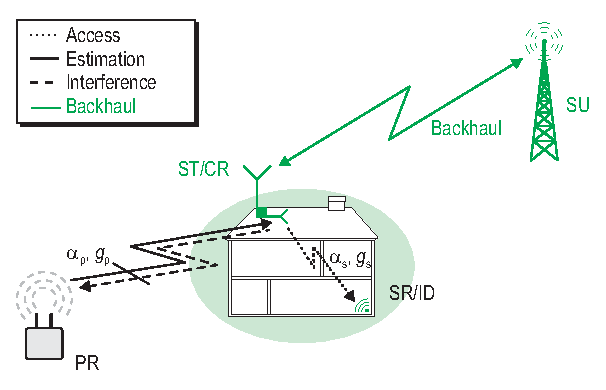
\includegraphics[width = \figscalet]{figures/CR_Scenario_Underlay}
%\vspace{-6mm}
\caption{A cognitive small cell scenario demonstrating: (i) the underlay paradigm, (ii) the associated network elements, which constitute Cognitive Small Cell-Base Station/Secondary Transmitter (CSC-BS/ST), Mobile Station/Secondary Receiver (MS/SR), Macro Cell-Base Station (MC-BS) and Primary Transmitter (PT), (iii) the interacting channels: primary interference channel, secondary interference channel and access channel.}
\label{fig:scenario}
%\vspace{-4mm}
\end{figure}
%\subsubsection{Medium access}

\subsection{Underlay Scenario and Medium Access}

Cognitive Small Cell (CSC), a CR application, characterizes a small cell deployment that fulfills the spectral requirements of the Mobile Stations (MSs) operating indoor, refer to \figurename~\ref{fig:scenario}.
For the disposition of the CSC in the network, the following key elements are essential: a CSC-Base Station (CSC-BS), a Macro Cell-Base Station (MC-BS) and an MS \cite{Kaushik16}.
Considering the fact that the power control is employed at the CSC-BS, the CSC-BS and the MS represent ST and SR, respectively. In order to acquire channel knowledge concerning the primary interference channel, the ST listens to the transmissions from the PR. In this work, we consider those primary systems where the PR performs transmissions interchangeably over time (time division duplexing TDD and half-duplex frequency division duplexing FDD) or frequency (full-duplex FDD) with the PT. These transmissions can occur over the same band (TDD) or over separate bands (half-duplex and full-duplex FDD). 
%The ST follows these duplexing modes to transmit signals with controlled power over the access channel. 
In cellular networks, these duplexing modes are effectively deployed in the Long Term Evolution (LTE) standard \cite{LTE09}. The ST follows these duplexing modes to exploit channel reciprocity principle and determine the primary interference (power) received at the PR, thus, controls its power for transmitting signals over the access channel such that it satisfies the interference constraint by operating at the IT. Particularly for half-duplex and full duplex FDD, it is assumed that the coherence bandwidth is large as compared to frequency separation between the estimation channel and the band of interest. 
%In addition, considering the deployment scenario, due to the outside walls, the SR encounters a loss of $\SI{20}{dB}$ in the received power, 
%Cognitive Relay (CR) \cite{Kaushik14} characterizes a small cell deployment that fulfills the spectral requirements for Indoor Devices (IDs). \figurename~\ref{fig:scenario} illustrates a snapshot of a CR scenario to depict the interaction between the CR with PR and ID, where CR and ID represents the ST and SR respectively. In \cite{Kaushik14}, the challenges involved while deploying the CR as US were presented. However for simplification, a constant transmit power was considered at the CR. Now, we extend the analysis to employ power control at the ST. 
%\begin{figure}[!t]
%\centering
%\includegraphics[width = \figscalet]{figures/Frame_Structure_ink}
%\vspace{-6mm}
%\caption{The proposed frame structure of underlay system channel estimation for the interference channel.}
%\label{fig:fs}
%\vspace{-11mm}
%\end{figure}
\begin{figure}[!t]
\centering
\includegraphics[width = 0.6 \columnwidth]{figures/Frame_Structure}
\caption{Frame structure of the USs illustrating the time allocation for channel estimation and data transmission from the perspective of a ST and a SR. In this regard, corresponding to the uplink and the downlink, the primary interference and secondary interference channel estimation occur at the ST and the SR, respectively. PR (Tx)/PR (Rx) presents the transmission/reception of the primary signal from the PR/PT to the PT/PR.} 
\label{fig:fs}
\vspace{-7mm}
\end{figure}



We propose to employ a slotted medium access for the US, where the time axis is segmented into frames. As depicted in \figurename~\ref{fig:fs}, the frame duration $T$ is chosen in such a way that the frames are aligned to the PUs' transmissions. In order to incorporate channel estimation, we further propose to employ a periodic channel estimation\footnote{This frame structure is similar to the periodic sensing followed by the interweave systems \cite{Liang08}.}, according to which, the US uses a time interval $\tau (< T)$ to perform channel estimation followed by data transmission $T- \tau$, see \figurename~\ref{fig:fs}. In order to consider variations due to channel fading, we assume that the interacting channels remain constant over two frame durations ($2T$). Based on this assumption, every alternating transmission frame observes a different received power, consider \figurename~\ref{fig:fs}. Since the channel knowledge is essential to employ power control such that the PUs are sufficiently protected from the excessive interference induced due to imperfect channel knowledge, it is reasonable to carry out estimation for $\tau$ time interval followed by data transmission with power control in the remaining time $T - \tau$ for each frame. %At the end, the remaining time $T - \tau$ is utilized for data transmission with controlled power. 

In accordance with the half duplexing modes, the ST and the SR perform received power estimation to acquire the knowledge of the primary and the secondary interference channel over consecutive frames, as illustrated in \figurename~\ref{fig:fs}. For primary systems and secondary systems that implement full-duplex FDD, the proposed frame structure can be adapted such that the primary and secondary interference channel estimation occurs in a single frame. Besides that, since the access channel estimation is performed by listening to the pilot symbols from the SR depicted as pilot based estimation, no time resources are allocated for access channel estimation in the frame structure, hence $\tau$ is utilized for the estimation of the interference channels only. 
At first, we consider the proposed frame structure for a short-term analysis, i.e., the performance is analyzed for a certain channel gain (deterministic channel), without taking into account the effect of channel fading. Next, by taking channel fading into account, we carry out a long-term analysis of the proposed framework. In accordance with the nature of regulatory policies, the aforementioned analyses can be considered for deploying the underlay CR systems. 



%To simplify the analysis, we assume that during data transmission at the ST, the interference at the SR, from the PT, to be below the noise level. However, by replacing the noise power with interference plus noise power in the throughput expressions, derived later in Section \ref{sec:et_ana}, the performance of the US under the interference limited regime can be depicted. %In this view, the interaction with the PT is excluded in the considered scenario, cf. \figurename~\ref{fig:scenario}. 

\subsection{Signal Model}
During the estimation phase, the discrete and complex signal received from the PR at the ST is given by
\begin{equation}
\yrcvd[n] = \gpo \cdot \xtran[n] + \nas[n],
\label{eq:sys_mod_st}
\end{equation}
where $\xtran[n]$ corresponds to a discrete and complex sample transmitted by the PR with transmit power $\ptran$ known at the ST, $\pgpo$ represents the power gain for the interference channel and $\nas[n]$ is circularly symmetric complex Additive White Gaussian Noise (AWGN) at the ST with %The transmitted power at PR is $\ptran$, considering that $\tau \fsam$ $(= N)$ is the number of samples used for estimation. 
$\mathcal{CN}(0, \nps)$. %The power received at the ST is given as 
%\begin{align}
%\prcvd = \s{\tau \fsam}{ |\sqrt{\gp \ap} \xtran[n] + \nas[n]|^2}.
%\label{eq:prcvd} 
%\end{align}

During data transmission phase, the interference signal received at the PR is given by
\begin{equation}
\yp[n] = \gpo  \cdot \xreg[n] + \nap[n],
\label{eq:sys_mod_pr}
\end{equation}
and on the other side, the received signal at the SR follows 
\begin{equation}
\ys[n] = \gs \cdot \xreg[n] + \gpt \cdot \xtran[n] + \nas[n],
\label{eq:sys_mod_sr}
\end{equation}
where $\xreg[n]$ corresponds to a discrete and complex sample transmitted by the ST with controlled power $\preg$, and $\xtran[n]$ is the transmit signal from the PT with transmit power $\ptran$\footnote{To avoid the use of an extra notation, we choose the transmit power to be the same for the PT and the PR, however, in practice, it might be different from the PR. In such situations also, for the proposed framework, its ignorance at the SR doesn't affect the analysis of the secondary interference.}. Further, $\pgs$ and $\pgpt$ represent the power gain for the access channel and the secondary interference channel, respectively and $\nap[n]$ is AWGN at the PR with $\mathcal{CN}(0, \nps)$. %The power received at the ST is given as 
%Considering (\ref{eq:sys_mod_pr}), the powers received at the PR and SR are evaluated as $\pp = \s{(T - \tau) \fsam}{|\yp[n]^2|}$ and $\ps = \s{(T - \tau) \fsam}{|\yp[n]^2|}$. Likewise (\ref{eq:sys_mod_st}), $\nap[n]$ and $\nas[n]$ represents circularly symmetric AWGN at PR and ST with zero mean and variance $\e{}{|\nap[n]|^2} = \npp$ and $\e{}{|\nas[n]|^2} = \nps$ correspondingly. Consider that $\ptran$, $\preg$ and $\pp$ correspond to power for a given frame. 
%\subsubsection{Channel}

%We consider that all transmitted signals are subjected to distance dependent path loss. The small scale fading gains $\gp, \gs$ are modelled as frequency-flat fading. Hence, the $\gp, \gs$ follow an exponential distribution \cite{Tse05} where $\e{}{\gp}$ and $\e{}{\gs}$ represent their path loss.

\subsection{Problem Description} \label{ssec:pd}
According to the existing investigations (also referred as ideal model), an ST of an US is required to control its transmit power in such a way that the primary interference (power) received $\pp$ at the PR is below IT $\ite$ \cite{Xing07}
\begin{equation}
\pp = \pgpo \preg \le \ite.
\label{eq:IT_id}
\end{equation}
%where $\alpha$ denotes the distance dependent path loss. $g\sub{p}$ represents the small-scale channel fading. 

With the controlled power at the ST determined using (\ref{eq:IT_id}), the capacity at the SR is defined as
\begin{equation}
\ca = \log_2 \left(1 + \frac{\pgs \preg}{ \pgpt \ptran + \nps} \right). 
\label{eq:Thr_id}
\end{equation}
%where $\e{\gs, \gp}{\cdot}$ represents the expectation over $\gs, \gp$.
From the deployment perspective, the ideal model depicted in (\ref{eq:IT_id}) and (\ref{eq:Thr_id}) has following issues:
\begin{itemize}
\item Without the knowledge of the primary interference channel $\gpo$, it is impossible to employ the power control based on (\ref{eq:IT_id}). 
\item Furthermore, along with $\preg$, the knowledge of the access channel $\gs$ and the secondary interference channel $\gpt$ is required to determine $\ca$ according to (\ref{eq:Thr_id}).
\end{itemize}
The ideal model considers the perfect knowledge of the aforementioned channels at the ST, which is not available in practice. In this regard, we incorporate channel estimation in the system model. The imperfect channel knowledge, however, translates to the variations in the performance parameters, $\pp$ and $\ca$. Particularly, a variation in $\pp$ that exceeds $\ite$ causes excessive interference at the PR, thereby violating the interference constraint illustrated in (\ref{eq:IT_id}). Unless captured, this excessive interference may seriously degrade the performance of the US. Since the ideal model assumes the perfect knowledge of the involved channels, it fails to depict the degradation in the performance due to the time resources allocated for the channel estimation. %In this view, we characterize the variations in $\pp$ and $\trs$ by characterizing the distribution functions of the estimated channels.

\subsection{Proposed Approach} 
In order to facilitate channel estimation for the USs, it is essential to take the aforementioned issues into account. To accomplish this, the following strategy is proposed in the paper.
\begin{itemize}
\item At first, we consider the estimation of involved channels. In this regard, we propose to employ a received power estimation for the interference channels and a pilot based estimation for the access channel. 
\item To capture the effect of the imperfect channel knowledge, we characterize the variations in the estimated parameters (namely, received power for the interference channels and power gain for the access channels) in terms of their cumulative distribution functions.
\item Further, we translate the aforementioned variations to the performance parameters, such as primary interference and secondary throughput in terms of their cumulative distribution functions. More specifically, using the characterization of the primary interference, we propose a novel power control mechanism that regulates the excessive interference at the PR.  
\item Finally, using the derived expressions, we analyze a relationship between the estimation time and the expected secondary throughput for the USs. We extend the proposed framework (also referred as estimation model) to analyze the impact of channel fading on the performance of the system. 
\end{itemize}
Since the channel estimation in the context of CR systems involves two different (primary and secondary) systems, the channel estimation techniques should be selected in such a way that (i) low complexity and (ii) versatility towards unknown PU signals requirements are respected. Similar situation, however, in context to interweave systems has been deeply investigated in \cite{Kaushik16}, according to which, the authors in \cite{Kaushik16} propose to employ a received power estimation for the channels between the primary and secondary users and a pilot based estimation for the access channel. In this paper, we propose to employ the channel estimation techniques in context to the underlay systems. It is also worth noticing that, since the signal model in \cite{Kaushik16} (Orthogonal Frequency Division Multiplexing transmission) differ from the one (constant power transmission) depicted in this paper, we derive new mathematical expressions for the derivation of the performance parameters. 
In the following paragraphs, we consider the estimation of the power gains of the primary interference channel $\epgpo$, the access channel $\epgs$ and the secondary interference channel $\epgpt$. 
\subsubsection{Estimation of primary interference channel}
Given 
\begin{equation}
\prcvd = \pgpo \ptran + \nps \label{eq:prcvd}, 
\end{equation}
and the knowledge of PR's transmit power $\ptran$, the ST listens to the transmissions from the PR and acquires the knowledge of $\epgpo$ indirectly by estimating the received power $\eprcvd = \s{\tau \fsam}{ |\yrcvd[n]|^2}$ in the uplink and perform data transmission with the controlled power over the downlink, refer to \figurename~\ref{fig:fs}, where $\fsam$ being the sampling frequency. Besides the knowledge of $\gpt$, the knowledge of $\ptran$ at the ST is critical for the employing the power control. However, this knowledge can be retrieved by considering the specifications of different wireless standards such GSM, EDGE and LTE, etc. \cite{Sharma14}. It is known that, certain standards are equipped with adaptive modulation and control, which can consequently change $\ptran$. Under these situations, the ST can employ adaptive modulation and classification techniques over the samples used for estimation in order to determine $\ptran$ based on the modulation order for the given frame \cite{Tsak14_}. 
%\begin{align}
%\eprcvd = \s{\tau \fsam}{ |\yrcvd[n]|^2}.
%\label{eq:prcvd} 
%\end{align}

$\eprcvd$ estimated using $\tau \fsam$ samples, refer to (\ref{eq:prcvd}), follows a non-central chi-squared distribution $\fprcvd \sim \ncchi2(\lpo, \tau \fsam)$ with a non-centrality parameter $\lpo = \tau \fsam \pgpo \ptran /\nps = \tau \fsam \gamma$ \cite{Kay}, where $\gamma$ is defined as the ratio of the received power (from the PR) to noise at the ST and $\tau \fsam$ corresponds to the degrees of freedom. For analytical tractability, we consider the following approximation. 
\begin{approxi} \label{ap:ap1}
\normalfont
For all degrees of freedom, the $\ncchi2$ distribution can be approximated by a Gamma distribution \cite{abramo}. The parameters of the Gamma distribution are obtained by matching the first two central moments to those of $\ncchi2$.
\end{approxi}
\begin{lemma} \label{lm:lm1}
\normalfont
The cumulative distribution function of $\eprcvd$ is characterized as 
\begin{align}
\fprcvd(x) \approx 1 - \Gamma&\left(\apo, \frac{x}{\bpo}\right) \label{eq:fprcvd}, \\ 
\text{where  } \apo = \frac{\tau \fsam (1 + \gamma)^2}{2 + 4 \gamma} &\text{ and } \bpo = \frac{\nps (2 + 4 \gamma)}{\tau \fsam (1 + \gamma)},  \label{eq:para_po} 
\end{align} 
and $\Gamma(\cdot, \cdot)$ represents the regularized upper-incomplete Gamma function \cite{abramo}. 
\end{lemma}
\begin{IEEEproof}
Applying Approximation \ref{ap:ap1} to $\ncchi2(\lpo, \tau \fsam)$ yields (\ref{eq:fprcvd}). 
\end{IEEEproof}

\subsubsection{Estimation of access channel}
In the uplink, the pilot signal received from the SR undergoes matched filtering and demodulation at the ST, hence, we employ a pilot-based estimation at the ST to acquire the knowledge of the access channel. According to \cite{Gifford08}, the maximum-likelihood estimate with $\Ks$ pilot symbols is given by 
\begin{align}
\gs = \egs + \frac{\sum^{\Ks}_{n} p[n]}{2 \Ks},
\label{eq:pilot_MLE}
\end{align}
where $p[n]$ denotes the discrete pilot symbol and $\frac{\sum^{\Ks}_{n} p[n]}{2 \Ks}$ represents the estimation error.
%(\ref{eq:pilot_MLE}) illustrates a correlation between the $\hs$ and $\ehs$. 
As a result, the estimate $\egs$ is unbiased, efficient, i.e., achieves the Cram\'er-Rao bound with equality, with asymptotic variance $\e{}{|\gs -\egs|^2} = \frac{\nps}{2 \Ks}$ \cite{Gifford08}. Hence, $\egs$ conditioned on $\gs$ follows a Gaussian distribution
\begin{align}
\egs|\gs \sim \mathcal{N}\left( \gs,\frac{\nps}{2 \Ks} \right).
\label{eq:ehs} 
\end{align}
Consequently, the estimated power gain $|\egs|^2$ follows a non-central chi-squared $\ncchi2(\ls, 1)$ distribution with 1 degree of freedom and non-centrality parameter $\ls = \frac{2 \Ks |\gs|^2}{\nps}$. 
\begin{lemma} \label{lm:lm2}
\normalfont
The cumulative distribution function of $\epgs$ is characterized as 
\begin{align}
\fgs(x) \approx 1 - \Gamma&\left(\as, \frac{x}{\bs}\right) \label{eq:fehs},\\ 
\text{where  } \as = \frac{(1 + \ls)^2}{2 + 4 \ls} &\text{ and } \bs = \frac{\nps (2 + 4 \ls)}{(1 + \ls)}. \label{eq:para_s} 
\end{align} 
\end{lemma}
\begin{IEEEproof}
Applying Approximation \ref{ap:ap1} to $\ncchi2(\ls,1 )$ yields (\ref{eq:fehs}). 
\end{IEEEproof}

\subsubsection{Estimation of secondary interference channel}
In the downlink, the SR cancels the ST pilot signal over the access channel in order to estimate the secondary interference (power) received from the PT, refer to (\ref{eq:sys_mod_sr}). The power estimated over the signal $\gpo \xtran[n]$ $+$ $\nas[n]$ corresponds to the interference plus noise power ($\eprcvdsr = \pgpt \ptran + \nps$, where $\prcvdsr$ represents the true value, consider (\ref{eq:Thr_id})). To characterize the secondary throughput, $\eprcvdsr$ is made available to the ST over a low rate feedback channel. Similar to $\eprcvd$, $\eprcvdsr$ follows a non-central chi-squared distribution $\ncchi2(\ls, \tau \fsam)$, wit non-centrality parameter $\lpt = \tau \fsam \pgpt \ptran / \nps$.
\begin{lemma} \label{lm:lm3}
\normalfont
The cumulative distribution function of $\eprcvd$ is characterized as 
\begin{align}
\fprcvdsr(x) \approx 1 - \Gamma&\left(\apt, \frac{x}{\bpt}\right) \label{eq:fprcvdsr}, \\ 
\text{where  } \apt = \frac{(\tau \fsam + \lpt)^2}{2 \tau \fsam + 4 \lpt} &\text{ and } \bpt = \frac{\nps (2 \tau \fsam + 4 \lpt)}{(\tau \fsam + \lpt)}.  \label{eq:para_pt} 
\end{align} 
\end{lemma}
\begin{IEEEproof}
Applying Approximation \ref{ap:ap1} to $\ncchi2(\lpt, \tau \fsam)$ yields (\ref{eq:fprcvdsr}). 
\end{IEEEproof}
It is important to note that, in this paper, we are dealing with a single PT and a single PR. However, in practice, it is possible that the ST and the SR accumulate significant interference (defined as aggregate interference) from other PRs and PTs (co-channel interference due to frequency reuse) in the network\cite{Elsawy13_cmag,Kaushik14_P} over the primary interference and the secondary interference channel, respectively. For the secondary interference channel, the only difference is that the SR now estimates the aggregate interference. Due to this, the expression of the $\eprcvdsr$ in the throughput remains unchanged. On the other side, by estimating the aggregate interference on the primary interference channel, the ST overestimates $\eprcvd$ and exercises a greater power control. Even for such a case, the outage constraint on the primary interference channel to the desired PR is satisfied, which consequently reduces the secondary throughput.  

%%%%%%%%%%%%%%%%%%%%%%%%%%%%%%%%%%%%%%%%%%%%%%%%%%%%%%%%%%%%%%%%%%%%%%%%%%%%%%%%%%%%%%%%%
\section{Theoretical Analysis} \label{sec:th_ana}
%%%%%%%%%%%%%%%%%%%%%%%%%%%%%%%%%%%%%%%%%%%%%%%%%%%%%%%%%%%%%%%%%%%%%%%%%%%%%%%%%%%%%%%%%

%%%%%%%%%%%%%%%%%%%%%%%%%%%%%%%%%%%%%%%%%%%%%%%%%%%%%%%%%%%%%%%%%%%%%%%%%%%%%%%%%%%%%%%%%
\subsection{Short-term Performance Analysis} \label{ssec:stpa}
%%%%%%%%%%%%%%%%%%%%%%%%%%%%%%%%%%%%%%%%%%%%%%%%%%%%%%%%%%%%%%%%%%%%%%%%%%%%%%%%%%%%%%%%%

%\subsection{Short-term Analysis}
%We first investigate the short-term analysis, whereby the channel is $\gp, \gs$ to a and unknown.
%  desired by the regulatory bodies, we capture this variation by means of an outage probability constraint $\p(\pp \ge \ite) \le \opc$.  %, it is important for the system to restrain $\op$ above a certain desired level $\opc$. %As a result, the outage probability constraint is defined as
%\begin{align}
%\p(\pp = \gp \preg \ge \ite) \le \opd. 
%\label{eq:opc} 
%\end{align} 
%\begin{lemma}
%The controlled power that satisfies 
%\end{lemma}
%\subsubsection{Power control}
%Given $\tau$ is utilized for $\prcvd$ estimation, the throughput at the SR is given by  
%\begin{equation}
%\rs(\tau) = \frac{T - \tau}{T} \log_2 \left(1 + \frac{\gs \preg(\tau) }{\nps} \right). 
%\label{eq:Thr_pm}
%\end{equation}
%It will be clear later in this section that small $\tau$ results in large variations for the $\prcvd$ and vice versa. According to (\ref{eq:preg}), this induces variations in $\preg$. These variations causes $\pp$ to deviate from $\ite$. If not considered in the model, these variations may affect the performance of the system. 
%Based on (\ref{eq:opc}), the controlled power at the PR is determined as 
%\begin{align}
%\preg(\tau) = \ite \cdot F_{\frac{1}{\gp}}^{-1}(\opd, \tau), 
%\label{eq:preg}
%\end{align}
%where $\mathcal{F}_{\frac{1}{\gp}}^{-1}$ represents the inverse-distribution function of $1/{\gp}$.
%Clearly, there exits a tradeoff that involves maximizing the expected throughput at the SR subject to a outage probability constraint is given by 
In this section, we investigate the performance of the USs for a certain frame. In this sense, the involved channels $\gpo$, $\gpt$ and $\gs$ are deterministic.   
At first, we employ an outage probability constraint\footnote{The outage constraint is commonly used parameter for designing communication system that ensures the outage occurs no more than a certain percentage of time.} $\opc$ on the primary interference to capture the variations in the $\pp$ incurred due to channel estimation, defined as 
\begin{align}
\p\left( \pp  (= \epgpo \preg) \ge \ite \right) \le \opc, \nonumber \\
\intertext{Substituting $\epgpo$ from (\ref{eq:prcvd}) yields}
\p\left( \left( \frac{\eprcvd - \nps}{\ptran}\right) \preg \ge \ite \right) \le \opc. \label{eq:opc} \\[-1em] \nonumber 
\end{align}
Besides the outage constraint, $\preg$ is limited by a predefined transmit power $\pc$. To capture this aspect, the transmit power constraint at the ST is defined as
\begin{align}
\preg \le \pc. \label{eq:pc} 
\end{align} 
Based on the aforementioned constraints, we determine the expression of the controlled power for the proposed framework.
\begin{lemma} \label{lm:lm4}
\normalfont
Subject to the outage constraint on the primary interference and the transmit power constraint at the ST, the controlled power at the ST is given by
\begin{align}
\preg &= 
\begin{cases} 
\frac{\ite \ptran}{ \left(\bpo \Gamma^{-1}(\opc, \apo) - \nps  \right)} & \mbox{if } \preg < \pc \\
\pc & \mbox{if } \preg \ge \pc
\end{cases},
\label{eq:preg} 
\end{align}
where $\apo$ and $\bpo$ are defined in (\ref{eq:para_po}) and $\Gamma^{-1}(\cdot, \cdot)$ is the inverse function of regularized upper-incomplete Gamma function \cite{abramo}.
\end{lemma} 
\begin{IEEEproof}
Substituting the distribution function for $\eprcvd$, defined in (\ref{eq:fprcvd}), in (\ref{eq:opc}) and combining with (\ref{eq:pc}) yields (\ref{eq:preg}).
\end{IEEEproof}
Clearly, $\preg$ increases with increase in $\pgpo$, which represent a low $\gamma$, which consequently enhances the performance in terms of the secondary throughput is achieved by the USs. However, due to the presence to $\pc$, the performance of the USs is constrained. In this regard, by substituting $\pc$ against $\preg$ determined in Lemma \ref{lm:lm4}, we determine a performance limit $(\gamma^*)$ of the US. 
\begin{coro} \label{cor:cor1}
\normalfont
Subject to the outage constraint on the primary interference and the transmit power constraint at the ST, the performance limit ($\gamma^*$) of the USs that employ power control at the secondary is defined as\footnote{Please note that $\tau \fsam$ and $\gamma$ are included in the parameters $\apo$ and $\bpo$, refer to (\ref{eq:para_po}).} 
\begin{align}
\Gamma\left(\apo, \frac{1}{\bpo} \left( \frac{\ite \ptran}{\pc} + \nps  \right)  \right) \le \opc. \label{eq:opreg}  
\end{align}
\end{coro}
\begin{IEEEproof}
Substituting $\preg$, refer to (\ref{eq:preg}), in (\ref{eq:pc}) results in (\ref{eq:opreg}). By replacing the expression in $(\ref{eq:opreg})$ with equality yields $\gamma^*$. 
\end{IEEEproof}

\begin{figure}
%\vspace{-5mm}
%% Add psfrag entries
% This file is generated by the MATLAB m-file laprint.m. It can be included
% into LaTeX documents using the packages graphicx, color and psfrag.
% It is accompanied by a postscript file. A sample LaTeX file is:
%    \documentclass{article}\usepackage{graphicx,color,psfrag}
%    \begin{document}% This file is generated by the MATLAB m-file laprint.m. It can be included
% into LaTeX documents using the packages graphicx, color and psfrag.
% It is accompanied by a postscript file. A sample LaTeX file is:
%    \documentclass{article}\usepackage{graphicx,color,psfrag}
%    \begin{document}% This file is generated by the MATLAB m-file laprint.m. It can be included
% into LaTeX documents using the packages graphicx, color and psfrag.
% It is accompanied by a postscript file. A sample LaTeX file is:
%    \documentclass{article}\usepackage{graphicx,color,psfrag}
%    \begin{document}\input{fig_N_vs_SNR_diff_pout_diff_maxContPow_th}\end{document}
% See http://www.mathworks.de/matlabcentral/fileexchange/loadFile.do?objectId=4638
% for recent versions of laprint.m.
%
% created by:           LaPrint version 3.16 (13.9.2004)
% created on:           06-Jan-2016 16:54:20
% eps bounding box:     16 cm x 12 cm
% comment:              
%
%\begin{psfrags}%
%\psfragscanon%
%
% text strings:
\psfrag{s03}[b][b]{\fontsize{8.5}{12.75}\fontseries{m}\mathversion{normal}\fontshape{n}\selectfont \color[rgb]{0,0,0}\setlength{\tabcolsep}{0pt}\begin{tabular}{c}$\tau$ [ms]\end{tabular}}%
\psfrag{s04}[t][t]{\fontsize{8.5}{12.75}\fontseries{m}\mathversion{normal}\fontshape{n}\selectfont \color[rgb]{0,0,0}\setlength{\tabcolsep}{0pt}\begin{tabular}{c}$\gamma$ [dB]\end{tabular}}%
%
% axes font properties:
\fontsize{8.5}{12.75}\fontseries{m}\mathversion{normal}%
\fontshape{n}\selectfont%
%
% xticklabels:
\psfrag{x01}[t][t]{-20}%
\psfrag{x02}[t][t]{-15}%
\psfrag{x03}[t][t]{-10}%
\psfrag{x04}[t][t]{-5}%
%
% yticklabels:
\psfrag{v01}[r][r]{0}%
\psfrag{v02}[r][r]{2}%
\psfrag{v03}[r][r]{4}%
\psfrag{v04}[r][r]{6}%
\psfrag{v05}[r][r]{8}%
\psfrag{v06}[r][r]{10}%
\psfrag{v07}[r][r]{12}%
\psfrag{v08}[r][r]{14}%
\psfrag{v09}[r][r]{16}%
\psfrag{v10}[r][r]{18}%
\psfrag{v11}[r][r]{20}%
%
% Figure:
%\resizebox{8cm}{!}{\includegraphics{fig_N_vs_SNR_diff_pout_diff_maxContPow_th.eps}}%
%\end{psfrags}%
%
% End fig_N_vs_SNR_diff_pout_diff_maxContPow_th.tex
\end{document}
% See http://www.mathworks.de/matlabcentral/fileexchange/loadFile.do?objectId=4638
% for recent versions of laprint.m.
%
% created by:           LaPrint version 3.16 (13.9.2004)
% created on:           06-Jan-2016 16:54:20
% eps bounding box:     16 cm x 12 cm
% comment:              
%
%\begin{psfrags}%
%\psfragscanon%
%
% text strings:
\psfrag{s03}[b][b]{\fontsize{8.5}{12.75}\fontseries{m}\mathversion{normal}\fontshape{n}\selectfont \color[rgb]{0,0,0}\setlength{\tabcolsep}{0pt}\begin{tabular}{c}$\tau$ [ms]\end{tabular}}%
\psfrag{s04}[t][t]{\fontsize{8.5}{12.75}\fontseries{m}\mathversion{normal}\fontshape{n}\selectfont \color[rgb]{0,0,0}\setlength{\tabcolsep}{0pt}\begin{tabular}{c}$\gamma$ [dB]\end{tabular}}%
%
% axes font properties:
\fontsize{8.5}{12.75}\fontseries{m}\mathversion{normal}%
\fontshape{n}\selectfont%
%
% xticklabels:
\psfrag{x01}[t][t]{-20}%
\psfrag{x02}[t][t]{-15}%
\psfrag{x03}[t][t]{-10}%
\psfrag{x04}[t][t]{-5}%
%
% yticklabels:
\psfrag{v01}[r][r]{0}%
\psfrag{v02}[r][r]{2}%
\psfrag{v03}[r][r]{4}%
\psfrag{v04}[r][r]{6}%
\psfrag{v05}[r][r]{8}%
\psfrag{v06}[r][r]{10}%
\psfrag{v07}[r][r]{12}%
\psfrag{v08}[r][r]{14}%
\psfrag{v09}[r][r]{16}%
\psfrag{v10}[r][r]{18}%
\psfrag{v11}[r][r]{20}%
%
% Figure:
%\resizebox{8cm}{!}{\includegraphics{fig_N_vs_SNR_diff_pout_diff_maxContPow_th.eps}}%
%\end{psfrags}%
%
% End fig_N_vs_SNR_diff_pout_diff_maxContPow_th.tex
\end{document}
% See http://www.mathworks.de/matlabcentral/fileexchange/loadFile.do?objectId=4638
% for recent versions of laprint.m.
%
% created by:           LaPrint version 3.16 (13.9.2004)
% created on:           06-Jan-2016 16:54:20
% eps bounding box:     16 cm x 12 cm
% comment:              
%
%\begin{psfrags}%
%\psfragscanon%
%
% text strings:
\psfrag{s03}[b][b]{\fontsize{8.5}{12.75}\fontseries{m}\mathversion{normal}\fontshape{n}\selectfont \color[rgb]{0,0,0}\setlength{\tabcolsep}{0pt}\begin{tabular}{c}$\tau$ [ms]\end{tabular}}%
\psfrag{s04}[t][t]{\fontsize{8.5}{12.75}\fontseries{m}\mathversion{normal}\fontshape{n}\selectfont \color[rgb]{0,0,0}\setlength{\tabcolsep}{0pt}\begin{tabular}{c}$\gamma$ [dB]\end{tabular}}%
%
% axes font properties:
\fontsize{8.5}{12.75}\fontseries{m}\mathversion{normal}%
\fontshape{n}\selectfont%
%
% xticklabels:
\psfrag{x01}[t][t]{-20}%
\psfrag{x02}[t][t]{-15}%
\psfrag{x03}[t][t]{-10}%
\psfrag{x04}[t][t]{-5}%
%
% yticklabels:
\psfrag{v01}[r][r]{0}%
\psfrag{v02}[r][r]{2}%
\psfrag{v03}[r][r]{4}%
\psfrag{v04}[r][r]{6}%
\psfrag{v05}[r][r]{8}%
\psfrag{v06}[r][r]{10}%
\psfrag{v07}[r][r]{12}%
\psfrag{v08}[r][r]{14}%
\psfrag{v09}[r][r]{16}%
\psfrag{v10}[r][r]{18}%
\psfrag{v11}[r][r]{20}%
%
% Figure:
%\resizebox{8cm}{!}{\includegraphics{fig_N_vs_SNR_diff_pout_diff_maxContPow_th.eps}}%
%\end{psfrags}%
%
% End fig_N_vs_SNR_diff_pout_diff_maxContPow_th.tex

\centering
\begin{tikzpicture}[scale=1]
\node[anchor=south west,inner sep=0] (image) at (0,0)
{
\includegraphics[width= \figscale]{figures/fig_N_vs_SNR_diff_pout_diff_maxContPow_th}
};
\begin{scope}[x={(image.south east)},y={(image.north west)}]

%\draw (0.86,0.42) arc(-250:70:0.04 and 0.02);
%\node[draw,fill=gray!10,font=\footnotesize] (text1) at (0.65,0.4) {$\pc = \SI{-10}{dBm}$};
%\draw[black, <-] (text1.east) -- (0.835,0.4);
%\draw (0.42,0.7) arc(-250:70:0.04 and 0.02);
%\node[draw,fill=gray!10,font=\footnotesize] (text2) at (0.65,0.68) {$\pc = \SI{0}{dBm}$};
%\draw[black, <-] (text2.west) -- (0.475,0.68);

\draw (0.62,0.75) arc(-250:70:0.03 and 0.015);
\node[draw,fill=gray!0,font=\footnotesize] (text1) at (0.56,0.735) {$\gamma^*$}; 
%\draw[black, <-] (text1.east) -- (0.46,0.7);
\node[draw,fill=gray!0,font=\footnotesize] at (0.8,0.53) {Operating Regime};
\node[draw,fill=gray!0,font=\footnotesize] at (0.35,0.53) {Non-operating Regime};

%\draw[help lines,xstep=.1,ystep=.1] (0,0) grid (1,1);
%\foreach \x in {0,1,...,9} { \node [anchor=north] at (\x/10,0) {0.\x}; }
%\foreach \y in {0,1,...,9} { \node [anchor=east] at (0,\y/10) {0.\y}; }
\end{scope}
\end{tikzpicture}

%\vspace{-4mm}
\caption{An illustration of the operating and the non-operating regimes ($\gamma^*$) for the US depicted in terms of estimation time ($\tau$) and the ratio of the received power (from the PR) to noise ($\gamma$) at the ST.}
\label{fig:or}
%\vspace{-10mm}
\end{figure}
\begin{remark} \label{rm:rm1}
\normalfont
\figurename~\ref{fig:or} analyzes the variations of $\gamma^*$ with $\tau$. Using the expression $\gamma^*$ obtained in Corollary \ref{cor:cor1}, we classify the operation of the USs into the following regimes: (i) operating regime and (ii) non-operating regime. Inside the operating regime, the system employs power control to satisfy the given outage constraint. At $\gamma^*$, the system operates at the maximum transmit power, i.e., without power control. On the other side, the region $\gamma \le \gamma*$, which depicts a bad link quality between the ST and the PR, hence, beneficial to the SU. In reality, due to transmit power constraint, this favorable conditions does not translate to any performance gain. Therefore, this regime is characterized as non-operating regime. %As a result, by replacing $\gamma^*$ in the following expression of secondary throughput, we determine the performance limits of operation for the US. 
\end{remark}
%Based on the operation regime, we determine best performance, in terms of the lowest operational SNR, achieved by the US. 

Next, we capture the variations in the secondary throughput in terms of its expected value. To accomplish this, we determine the cumulative distribution function (cdf) of the capacity $\ca$ over the access channel.

\begin{lemma} \label{lm:lm5}
\normalfont
The cdf of capacity $\ca = \log_2 \left(1 + \frac{\epgs \ptran}{\eprcvdsr} \right)$ is given by
\begin{align}
\fc(x) &= \int\limits_{0}^{x} \dc(t) dt, \label{eq:dis_C} 
\end{align}
where the $\dc(x)$ probability density function (pdf) is given by 
\begin{align}
\dc(x) &= 2^x \ln 2 \frac{(2^x - 1)^{\as - 1} \Gamma(\as + \apt)}{\Gamma(\as) \Gamma(\apt) (\bs \ptran) ^{\as} \bpt^{\apt}} \left(\frac{1}{\bpt} + \frac{2^x - 1}{\bs \ptran}\right). \label{eq:den_C}
\end{align}
\end{lemma}
\begin{IEEEproof}
See Appendix \ref{ap:one}.
\end{IEEEproof}
Besides the outage constraint on the primary interference, the expected secondary throughput over the access channel at the SR is defined as
\begin{align}
\rs(\tau) = \e{\ca} {\frac{T - \tau}{T} \log_2 \left(1 + \frac{\epgs \preg }{\eprcvdsr} \right)}, \label{eq:rs}
\end{align} 
where $\e{\ca}{\cdot}$ corresponds to an expectation over $\ca$, whose pdf is characterized in Lemma \ref{lm:lm5}. 

At this stage, it is worthy to note that $\preg$ and $\trs$ depend on $\tau$, refer to (\ref{eq:preg}) and (\ref{eq:rs}), respectively. Hence, the proposed framework demostrates a fundamental tradeoff between the estimation time and the achievable secondary throughput.  
\begin{theorem} \label{th:th1}
\normalfont
The expected achievable secondary throughput subject to the outage constraint on the primary interference and the transmit power constraint at the ST is defined as
\begin{align}
\trs(\ttau) = \maxi_{\tau}  & \text{      } {\rs(\tau)}, 
 \label{eq:sys} \\
\text{s.t.} & \text{ } (\ref{eq:opc}), \text{  } (\ref{eq:pc}), \nonumber 
%\text{s.t.} & \text{ } \p\left( \left( \frac{\eprcvd - \nps}{\ptran} \right) \preg \ge \ite \right) \le \opc, \nonumber \\ 
%\text{s.t.} & \text{ }  \preg \le \pc, \nonumber   
 \end{align}
where $\trs(\ttau)$ corresponds to optimum throughput at $\ttau$.  
\end{theorem}
\begin{IEEEproof}
The constrained optimization problem is solved by substituting $\preg$ from Lemma \ref{lm:lm3}, determined by applying the outage and the transmit power constraints defined in (\ref{eq:opc}) and (\ref{eq:pc}), in (\ref{eq:rs}). 
The pdf of $\ca$, determined in (\ref{eq:den_C}), is used to evaluate the expectation. Following this, we obtain an expression of the expected secondary throughput as a function of $\tau$\footnote{Please note that $\apt$ and $\bpt$ are also functions of $\tau$, see (\ref{eq:para_pt}).}
\begin{equation}
\rs(\tau) = \frac{T - \tau}{T} \int\limits_{0}^{\infty} x \dc(x) dx. \label{eq:intrs}
\end{equation}
Solving numerically the expression in (\ref{eq:intrs}) yields $\ttau$ and $\trs(\ttau)$. 
\end{IEEEproof}
\begin{coro} \label{cor:cor2}
\normalfont
Theorem \ref{th:th1} considers the optimization of the expected secondary throughput for the proposed framework that employ power control and considers the effect of the imperfect channel knowledge. In this context, it is interesting to compare its performance with those CR systems that employ channel estimation (as proposed in the paper) and satisfy the outage constraint on the primary interference, however, operate at constant power $(= \pc)$. For this new approach, the secondary throughput is obtained by substituting the expression of $\pc$ in (\ref{eq:rs}), where $\tau$ in (\ref{eq:rs}) is determined using Corollary \ref{cor:cor1}. 
\end{coro}

%Theorem \ref{th:th1} depicts an optimum estimation time $\ttau$ that achieves an optimum secondary throughput $\trs(\ttau)$.
%The throughput depicted from (\ref{eq:Thr_id}) for the ideal model overestimates the throughput of the US. %This overestimation in the throughput is evaluated as $\beta$ that depicts the difference between the $\ers$ obtained from the models. 
%It is evident that for analyzing the tradeoff depicted in (\ref{eq:sys}), first it is important to characterize the $\preg$ and density function $\drs$. 

%\subsection{Short term analysis}
%To simplify the analysis, we consider a case where the transmitted signals are subject to path loss only, that is, the small scale channel gains correspond to $\gs = \gp = 1$. In this way, we first consider the variations in $\pp$ due to the presence of noise in the system. 

%\subsubsection{Characterization of performance parameters}
%Considering (\ref{eq:prcvd}), $\prcvd$ follows a non-central chi-squared distributed $\mathcal{X'}^2(N \gamma, N)$, where $\gamma = \ptran/\nps$ denotes the received SNR \cite{Urkowitz}. 
%According to (\ref{eq:preg}), $\preg$ for the short term case is given by 



%%%%%%%%%%%%%%%%%%%%%%%%%%%%%%%%%%%%%%%%%%%%%%%%%%%%%%%%%%%%%%%%%%%%%%%%%%%%%%%%%%%%%%%%%
\subsection{Long-term Performance Analysis}\label{ssec:ltpa}
%%%%%%%%%%%%%%%%%%%%%%%%%%%%%%%%%%%%%%%%%%%%%%%%%%%%%%%%%%%%%%%%%%%%%%%%%%%%%%%%%%%%%%%%%
Here, our objective is to investigate the long-term performance of the proposed approach. In this regard, we consider that the channel gains $\gpo$, $\gpt$ and $\gs$ are subject to Nakagami-$m$ fading model. As a consequence, the power gains $\pgpo$, $\pgpt$ and $\pgs$ follow a Gamma distribution \cite{Goldsmith05}, whose corresponding cumulative distribution functions are defined as  
\begin{align}
\fpgpo(x) = \gamma\left(\mpo, \frac{\mpo x}{\pgpo}\right), \label{eq:dis_pgpo}\\
\fpgpt(x) = \gamma\left(\mpt, \frac{\mpt x}{\pgpt}\right), \label{eq:dis_pgpt}\\  
\fpgs(x) = \gamma\left(\ms , \frac{\ms x}{\pgs}\right), \label{eq:dis_pgs}
\end{align}
where $\mpo$, $\mpt$ and $\ms$ represent the $m$ parameter for $\pgpo$, $\pgpt$ and $\pgs$, respectively, and $\gamma(\cdot, \cdot)$ is a regularized lower-incomplete Gamma function \cite{abramo}. The performance analysis subject to channel fading has been considered by Ghasemi \textit{et al.} \cite{Ghasemi06, Ghasemi07}. However, the authors in \cite{Ghasemi06, Ghasemi07} evaluated average capacity under an average interference constraint. The influence of channel fading (however, without channel estimation) has been quantified in terms of the outage constraint on the primary interference, is given by %. In order to make a fair comparison (benchmark) of our proposed approach, the ideal model the existing investigations in context to channel fading are quantified based on an outage constraint on the primary interference, given by
\begin{align}
	\quad & \e{\pgpt, \pgs }{ \ca(\pgpt, \pgs)} \label{eq:sys_id_fad}, \\
	\text{s.t.} & \text{ } \p(\pp(\pgpo) \ge \ite) \le \opc, \label{eq:opc_id_fad} 
\end{align}
where $\e{\pgpt, \pgs} {\cdot}$ corresponds to expectation with respect to $\pgpt, \pgs$.
Despite the knowledge of the fading model, similar to ideal model depicted in short-term analysis (refer to Section \ref{ssec:pd}), the characterization in (\ref{eq:sys_id_fad}) and (\ref{eq:opc_id_fad}) assumes the perfect knowledge\footnote{For the long-term analysis (or a fading channel), this knowledge signifies the expected values.} of the power gains $(\pgpo, \pgpt, \pgs)$ of the corresponding channels. In view of this, we extend our proposed framework to investigate the effect of the random channel (channel fading) on the performance of the USs.

In this regard, we first determine the expression of the outage constraint on the primary interference  
\begin{align}
\e{\pgpo}{\p\left( \left( \frac{\eprcvd(\pgpo) - \nps}{\ptran}\right) \preg \ge \ite \right)} \le \opc. \label{eq:opc_fad} 
\end{align}
In contrast to the constraint in (\ref{eq:opc_id_fad}), (\ref{eq:opc_fad}) considers the expectation $\e{\pgpo}{\cdot}$ over the estimated value of the channel $\epgpo$, determined in terms of $\eprcvd$. 
Based on (\ref{eq:opc_fad}) and transmit power constraint defined in (\ref{eq:pc}), we obtain the expression of the controlled power for the long-term analysis.

\begin{lemma} \label{lm:lm6}
\normalfont
Subject to the outage constraint on the primary interference and the transmit power constraint at the ST, the controlled power at the ST under Nakagami-$m$ fading is given by
%\begin{figure*}
\begin{align}
\preg &= 
\begin{cases} 
\text{Solving for $\preg$, } \\ \int\limits_{0}^{\infty} \Gamma\left(\apt(\pgpo), \frac{1}{\bpo(\pgpo)} \left(\frac{\ite\ptran}{\preg} + \nps \right)\right) d \fpgpo = \opc & \mbox{if } \preg < \pc \\
\pc & \mbox{if } \preg \ge \pc
\end{cases},
\label{eq:preg_fad} 
\end{align}
%\end{figure*}
where $\apo$ and $\bpo$ are defined in (\ref{eq:para_po}) and $\fpgpo(\cdot)$ is defined in (\ref{eq:dis_pgpo}). 
\end{lemma} 
\begin{IEEEproof}
Since it is complicated to obtain a closed form expression of the integral in (\ref{eq:preg_fad}), we evaluate the controlled power numerically.  
\end{IEEEproof}

Substituting $\preg$ with $\pc$ in the expression (\ref{eq:preg_fad}), the performance limit $\gamma^*$ for the long-term analysis is determined as
\begin{equation}
\int\limits_{0}^{\infty} \Gamma\left(\apt(\pgpo), \frac{1}{\bpo(\pgpo)} \left(\frac{\ite\ptran}{\pc} + \nps \right)\right) d \fpgpo \le \opc. \label{eq:or_fad}
\end{equation}

\begin{figure}

%% Add psfrag entries
% This file is generated by the MATLAB m-file laprint.m. It can be included
% into LaTeX documents using the packages graphicx, color and psfrag.
% It is accompanied by a postscript file. A sample LaTeX file is:
%    \documentclass{article}\usepackage{graphicx,color,psfrag}
%    \begin{document}% This file is generated by the MATLAB m-file laprint.m. It can be included
% into LaTeX documents using the packages graphicx, color and psfrag.
% It is accompanied by a postscript file. A sample LaTeX file is:
%    \documentclass{article}\usepackage{graphicx,color,psfrag}
%    \begin{document}% This file is generated by the MATLAB m-file laprint.m. It can be included
% into LaTeX documents using the packages graphicx, color and psfrag.
% It is accompanied by a postscript file. A sample LaTeX file is:
%    \documentclass{article}\usepackage{graphicx,color,psfrag}
%    \begin{document}\input{fig_N_vs_SNR_diff_pout_diff_maxContPow_fading_th}\end{document}
% See http://www.mathworks.de/matlabcentral/fileexchange/loadFile.do?objectId=4638
% for recent versions of laprint.m.
%
% created by:           LaPrint version 3.16 (13.9.2004)
% created on:           06-Jan-2016 11:22:04
% eps bounding box:     16 cm x 12 cm
% comment:              
%
%\begin{psfrags}%
%\psfragscanon%
%
% text strings:
\psfrag{s03}[b][b]{\fontsize{8}{12}\fontseries{m}\mathversion{normal}\fontshape{n}\selectfont \color[rgb]{0,0,0}\setlength{\tabcolsep}{0pt}\begin{tabular}{c}$\tau$ [ms]\end{tabular}}%
\psfrag{s04}[t][t]{\fontsize{8}{12}\fontseries{m}\mathversion{normal}\fontshape{n}\selectfont \color[rgb]{0,0,0}\setlength{\tabcolsep}{0pt}\begin{tabular}{c}$\gamma$ [dB]\end{tabular}}%
%
% axes font properties:
\fontsize{8}{12}\fontseries{m}\mathversion{normal}%
\fontshape{n}\selectfont%
%
% xticklabels:
\psfrag{x01}[t][t]{-20}%
\psfrag{x02}[t][t]{-19}%
\psfrag{x03}[t][t]{-18}%
\psfrag{x04}[t][t]{-17}%
\psfrag{x05}[t][t]{-16}%
\psfrag{x06}[t][t]{-15}%
\psfrag{x07}[t][t]{-14}%
\psfrag{x08}[t][t]{-13}%
\psfrag{x09}[t][t]{-12}%
\psfrag{x10}[t][t]{-11}%
\psfrag{x11}[t][t]{-10}%
%
% yticklabels:
\psfrag{v01}[r][r]{0}%
\psfrag{v02}[r][r]{2}%
\psfrag{v03}[r][r]{4}%
\psfrag{v04}[r][r]{6}%
\psfrag{v05}[r][r]{8}%
\psfrag{v06}[r][r]{10}%
\psfrag{v07}[r][r]{12}%
\psfrag{v08}[r][r]{14}%
\psfrag{v09}[r][r]{16}%
\psfrag{v10}[r][r]{18}%
\psfrag{v11}[r][r]{20}%
%
% Figure:
%\resizebox{8cm}{!}{\includegraphics{fig_N_vs_SNR_diff_pout_diff_maxContPow_fading_th.eps}}%
%\end{psfrags}%
%
% End fig_N_vs_SNR_diff_pout_diff_maxContPow_fading_th.tex
\end{document}
% See http://www.mathworks.de/matlabcentral/fileexchange/loadFile.do?objectId=4638
% for recent versions of laprint.m.
%
% created by:           LaPrint version 3.16 (13.9.2004)
% created on:           06-Jan-2016 11:22:04
% eps bounding box:     16 cm x 12 cm
% comment:              
%
%\begin{psfrags}%
%\psfragscanon%
%
% text strings:
\psfrag{s03}[b][b]{\fontsize{8}{12}\fontseries{m}\mathversion{normal}\fontshape{n}\selectfont \color[rgb]{0,0,0}\setlength{\tabcolsep}{0pt}\begin{tabular}{c}$\tau$ [ms]\end{tabular}}%
\psfrag{s04}[t][t]{\fontsize{8}{12}\fontseries{m}\mathversion{normal}\fontshape{n}\selectfont \color[rgb]{0,0,0}\setlength{\tabcolsep}{0pt}\begin{tabular}{c}$\gamma$ [dB]\end{tabular}}%
%
% axes font properties:
\fontsize{8}{12}\fontseries{m}\mathversion{normal}%
\fontshape{n}\selectfont%
%
% xticklabels:
\psfrag{x01}[t][t]{-20}%
\psfrag{x02}[t][t]{-19}%
\psfrag{x03}[t][t]{-18}%
\psfrag{x04}[t][t]{-17}%
\psfrag{x05}[t][t]{-16}%
\psfrag{x06}[t][t]{-15}%
\psfrag{x07}[t][t]{-14}%
\psfrag{x08}[t][t]{-13}%
\psfrag{x09}[t][t]{-12}%
\psfrag{x10}[t][t]{-11}%
\psfrag{x11}[t][t]{-10}%
%
% yticklabels:
\psfrag{v01}[r][r]{0}%
\psfrag{v02}[r][r]{2}%
\psfrag{v03}[r][r]{4}%
\psfrag{v04}[r][r]{6}%
\psfrag{v05}[r][r]{8}%
\psfrag{v06}[r][r]{10}%
\psfrag{v07}[r][r]{12}%
\psfrag{v08}[r][r]{14}%
\psfrag{v09}[r][r]{16}%
\psfrag{v10}[r][r]{18}%
\psfrag{v11}[r][r]{20}%
%
% Figure:
%\resizebox{8cm}{!}{\includegraphics{fig_N_vs_SNR_diff_pout_diff_maxContPow_fading_th.eps}}%
%\end{psfrags}%
%
% End fig_N_vs_SNR_diff_pout_diff_maxContPow_fading_th.tex
\end{document}
% See http://www.mathworks.de/matlabcentral/fileexchange/loadFile.do?objectId=4638
% for recent versions of laprint.m.
%
% created by:           LaPrint version 3.16 (13.9.2004)
% created on:           06-Jan-2016 11:22:04
% eps bounding box:     16 cm x 12 cm
% comment:              
%
%\begin{psfrags}%
%\psfragscanon%
%
% text strings:
\psfrag{s03}[b][b]{\fontsize{8}{12}\fontseries{m}\mathversion{normal}\fontshape{n}\selectfont \color[rgb]{0,0,0}\setlength{\tabcolsep}{0pt}\begin{tabular}{c}$\tau$ [ms]\end{tabular}}%
\psfrag{s04}[t][t]{\fontsize{8}{12}\fontseries{m}\mathversion{normal}\fontshape{n}\selectfont \color[rgb]{0,0,0}\setlength{\tabcolsep}{0pt}\begin{tabular}{c}$\gamma$ [dB]\end{tabular}}%
%
% axes font properties:
\fontsize{8}{12}\fontseries{m}\mathversion{normal}%
\fontshape{n}\selectfont%
%
% xticklabels:
\psfrag{x01}[t][t]{-20}%
\psfrag{x02}[t][t]{-19}%
\psfrag{x03}[t][t]{-18}%
\psfrag{x04}[t][t]{-17}%
\psfrag{x05}[t][t]{-16}%
\psfrag{x06}[t][t]{-15}%
\psfrag{x07}[t][t]{-14}%
\psfrag{x08}[t][t]{-13}%
\psfrag{x09}[t][t]{-12}%
\psfrag{x10}[t][t]{-11}%
\psfrag{x11}[t][t]{-10}%
%
% yticklabels:
\psfrag{v01}[r][r]{0}%
\psfrag{v02}[r][r]{2}%
\psfrag{v03}[r][r]{4}%
\psfrag{v04}[r][r]{6}%
\psfrag{v05}[r][r]{8}%
\psfrag{v06}[r][r]{10}%
\psfrag{v07}[r][r]{12}%
\psfrag{v08}[r][r]{14}%
\psfrag{v09}[r][r]{16}%
\psfrag{v10}[r][r]{18}%
\psfrag{v11}[r][r]{20}%
%
% Figure:
%\resizebox{8cm}{!}{\includegraphics{fig_N_vs_SNR_diff_pout_diff_maxContPow_fading_th.eps}}%
%\end{psfrags}%
%
% End fig_N_vs_SNR_diff_pout_diff_maxContPow_fading_th.tex

\centering
\begin{tikzpicture}[scale=1]
\node[anchor=south west,inner sep=0] (image) at (0,0)
{
\includegraphics[width= \figscale]{figures/fig_N_vs_SNR_diff_pout_diff_maxContPow_fading_th}
};
\begin{scope}[x={(image.south east)},y={(image.north west)}]

\draw (0.665,0.82) arc(-250:70:0.2 and 0.05);
\node[draw,fill=gray!10,font=\footnotesize] (text1) at (0.505,0.775) {$\gamma^*$};
%\draw[black,->] (0.12,0.2) node[below=4.0,right=-5.0, rotate = 75, font=\footnotesize] {$m \in \{0.5, 1,2,5, \infty\}$} -- (0.34,0.14);
\draw[black,->] (0.52,0.31) -- (0.85,0.2);
\node[rotate = 75, font=\footnotesize] at (0.5, 0.38) {$m \in \{0.5, 1,2,5, \infty\}$}; 
%\draw[help lines,xstep=.1,ystep=.1] (0,0) grid (1,1);
%\foreach \x in {0,1,...,9} { \node [anchor=north] at (\x/10,0) {0.\x}; }
%\foreach \y in {0,1,...,9} { \node [anchor=east] at (0,\y/10) {0.\y}; }
\end{scope}
\end{tikzpicture}
\caption{An extension of the operating and the non-operating regimes for the US to the random channels, where the channels are subject to Nakagami-$m$ fading. The performance limit ($\gamma^*$) is depicted in terms of estimation time ($\tau$). The different curves demonstrates the severity $(m \in \{0,5,1,2,5, \infty \})$ in fading observed by the channels.}
\label{fig:or_fad}
%\vspace{-5mm}
\end{figure}
\begin{remark} \label{rm:rm2}
\normalfont
\figurename~\ref{fig:or_fad} analyzes the variation of $\gamma^*$ with $\tau$ for different $m \in \{0.5, 1, 2, 5, \infty\}$, where $m = \infty$ depicts a path-loss channel (or converges to a deterministic channel). It is observed that $\gamma^*$ attains a lower value as fading becomes more severe, hence enables the USs to operate at low $\gamma$ by extending the operating regime. In addition, it is noticed that the path-loss channel is more sensitive to the estimation time as compared to the fading channels.  
\end{remark}

Upon determining the controlled power in Lemma \ref{lm:lm6} that constrains the primary interference, we determine the expression of the secondary throughput.
\begin{align}
\rs(\tau) &= \e{\ca, \pgpt, \pgs} {\frac{T - \tau}{T} \log_2 \left(1 + \frac{\epgs \preg }{\eprcvd(\pgpt)} \right)}, \label{eq:rs_fad} 
\end{align} 
where $\e{\ca, \pgpt, \pgs}{\cdot}$ corresponds to an expectation over $\ca$, $\pgpt, \pgs$, whose cdfs are characterized in Lemma \ref{lm:lm5}, (\ref{eq:dis_pgpt}) and (\ref{eq:dis_pgs}), respectively. It is worth noticing that $\ca$ entails the variations due to channel estimation $\epgs$ and $\eprcvd$.
Next, we characterize the estimation-throughput tradeoff for the long-term analysis of the proposed framework. 
\begin{theorem} \label{th:th2}
\normalfont
The expected achievable secondary throughput subject to the outage constraint on the primary interference and the transmit power constraint at the ST under Nakagami-$m$ fading is defined as
\begin{align}
\trs(\ttau) = \maxi_{\tau}  & \text{      } {\rs(\tau)}, 
 \label{eq:sys_fad} \\
\text{s.t.} & \text{ } (\ref{eq:opc_fad}), \text{  } (\ref{eq:pc}), \nonumber 
%\text{s.t.} & \text{ } \p\left( \left( \frac{\eprcvd - \nps}{\ptran} \right) \preg \ge \ite \right) \le \opc, \nonumber \\ 
%\text{s.t.} & \text{ }  \preg \le \pc, \nonumber   
 \end{align}
where $\trs(\ttau)$ corresponds to optimum throughput at $\ttau$.  
\end{theorem}

\begin{coro} \label{cor:cor3}
\normalfont
Here, we extend the approach depicted Corollary \ref{cor:cor2} to compare the performance with those CR systems that employ channel estimation, operate at constant power, satisfy the outage constraint and are subjected to Nakagami-$m$ fading. The expected secondary throughput for this particular approach is obtained by replacing $\preg$ in the expression in (\ref{eq:rs_fad}) with $\pc$, where $\tau$ is determined using (\ref{eq:or_fad}). 

\end{coro}
 
%%%%%%%%%%%%%%%%%%%%%%%%%%%%%%%%%%%%%%%%%%%%%%%%%%%%%%%%%%%%%%%%%%%%%%%%%%%%%%%%%%%%%%%%%
\section{Numerical Analysis} \label{sec:num_ana}
%%%%%%%%%%%%%%%%%%%%%%%%%%%%%%%%%%%%%%%%%%%%%%%%%%%%%%%%%%%%%%%%%%%%%%%%%%%%%%%%%%%%%%%%%
Here, we evaluate the performance of the US based on the proposed model. To accomplish this: (i) we perform simulations to validate the expressions obtained, (ii) we analyze the performance loss incurred due to the estimation. In addition, we consider the ideal model to benchmark and evaluate the performance loss. % (iii) we establish mathematical justification to the considered approximations.
% Unless stated explicitly, the following choice of the parameters is considered for the analysis, cf. Table \ref{tb:tb2}.
Unless stated explicitly, the parameters given in Table \ref{tb:tb2} are considered for the analysis.%, $\fsam = \SI{1}{MHz}$, $\gp = \SI{-100}{dB}$, $\gs = \SI{-80}{dB}$, $\ite = \SI{-110}{dBm}$, $T = \SI{100}{ms}$, $\opc \in \{0.01, 0.10\}$, $\pc \in \{-10, 0\} \SI{}{dBm}$, $\nps = \SI{-100}{dBm}$, $\gamma = \SI{0}{dB}$, $\ptran = \SI{0}{dBm}$, $\Ks = 10$.


%\subsection{Short-term analysis}

\begin{table}
%%\vspace{-0.4cm}
\renewcommand{\arraystretch}{1.2}
\caption{Parameters for Numerical Analysis}
%\vspace{-0.6cm}
\label{tb:tb2}
\centering
%\footnotesize{
\begin{tabular}{c||c}
\hline
\bfseries Parameter & \bfseries Value \\
\hline\hline
$\fsam$  & $\SI{1}{MHz}$ \\ 
$\pgpo$ & $\SI{-100}{dB}$ \\ 
$\pgpt$ & $\SI{-100}{dB}$ \\ 
$\pgs$ & $\SI{-80}{dB}$ \\ 
$\ite$ & $\SI{-110}{dBm}$ \\ 
$T$ & $\SI{100}{ms}$ \\ 
$\opc$ & 0.10 \\ 
$\pc$ & 0 \SI{}{dBm} \\ 
$\nps$ & $\SI{-100}{dBm}$ \\ 
$\gamma$ & $\SI{0}{dB}$ \\ 
$\ptran$ & $\SI{0}{dBm}$ \\ 
$\Ks$ & 10 \\ 
$m$ & \{1,5\} \\ \hline
\end{tabular}%}
\end{table}

%%%%%%%%%%%%%%%%%%%%%%%%%%%%%%%%%%%%%%%%%%%%%%%%%%%%%%%%%%%%%%%%%%%%%%%%%%%%%%%%%%%%%%%%%
\subsection{Short-term analysis} 
%%%%%%%%%%%%%%%%%%%%%%%%%%%%%%%%%%%%%%%%%%%%%%%%%%%%%%%%%%%%%%%%%%%%%%%%%%%%%%%%%%%%%%%%%

\begin{figure}
%% Add psfrag entries
% This file is generated by the MATLAB m-file laprint.m. It can be included
% into LaTeX documents using the packages graphicx, color and psfrag.
% It is accompanied by a postscript file. A sample LaTeX file is:
%    \documentclass{article}\usepackage{graphicx,color,psfrag}
%    \begin{document}% This file is generated by the MATLAB m-file laprint.m. It can be included
% into LaTeX documents using the packages graphicx, color and psfrag.
% It is accompanied by a postscript file. A sample LaTeX file is:
%    \documentclass{article}\usepackage{graphicx,color,psfrag}
%    \begin{document}% This file is generated by the MATLAB m-file laprint.m. It can be included
% into LaTeX documents using the packages graphicx, color and psfrag.
% It is accompanied by a postscript file. A sample LaTeX file is:
%    \documentclass{article}\usepackage{graphicx,color,psfrag}
%    \begin{document}\input{fig_Preg_est_time_AWGN}\end{document}
% See http://www.mathworks.de/matlabcentral/fileexchange/loadFile.do?objectId=4638
% for recent versions of laprint.m.
%
% created by:           LaPrint version 3.16 (13.9.2004)
% created on:           15-Dec-2015 22:25:07
% eps bounding box:     16 cm x 12 cm
% comment:              
%
%\begin{psfrags}%
%\psfragscanon%
%
% text strings:
\psfrag{s05}[b][b]{\fontsize{8.5}{12.75}\fontseries{m}\mathversion{normal}\fontshape{n}\selectfont \color[rgb]{0,0,0}\setlength{\tabcolsep}{0pt}\begin{tabular}{c}$\preg$ [dBm]\end{tabular}}%
\psfrag{s06}[t][t]{\fontsize{8.5}{12.75}\fontseries{m}\mathversion{normal}\fontshape{n}\selectfont \color[rgb]{0,0,0}\setlength{\tabcolsep}{0pt}\begin{tabular}{c}$\tau$ [ms]\end{tabular}}%
\psfrag{s10}[][]{\fontsize{10}{15}\fontseries{m}\mathversion{normal}\fontshape{n}\selectfont \color[rgb]{0,0,0}\setlength{\tabcolsep}{0pt}\begin{tabular}{c} \end{tabular}}%
\psfrag{s11}[][]{\fontsize{10}{15}\fontseries{m}\mathversion{normal}\fontshape{n}\selectfont \color[rgb]{0,0,0}\setlength{\tabcolsep}{0pt}\begin{tabular}{c} \end{tabular}}%
\psfrag{s12}[l][l]{\fontsize{8.5}{12.75}\fontseries{m}\mathversion{normal}\fontshape{n}\selectfont \color[rgb]{0,0,0}EM}%
\psfrag{s13}[l][l]{\fontsize{8.5}{12.75}\fontseries{m}\mathversion{normal}\fontshape{n}\selectfont \color[rgb]{0,0,0}IM}%
\psfrag{s14}[l][l]{\fontsize{8.5}{12.75}\fontseries{m}\mathversion{normal}\fontshape{n}\selectfont \color[rgb]{0,0,0}EM}%
%
% axes font properties:
\fontsize{8.5}{12.75}\fontseries{m}\mathversion{normal}%
\fontshape{n}\selectfont%
%
% xticklabels:
\psfrag{x01}[t][t]{$10^{-3}$}%
\psfrag{x02}[t][t]{$10^{-2}$}%
\psfrag{x03}[t][t]{$10^{-1}$}%
\psfrag{x04}[t][t]{$10^{0}$}%
\psfrag{x05}[t][t]{$10^{1}$}%
%
% yticklabels:
\psfrag{v01}[r][r]{-20}%
\psfrag{v02}[r][r]{-19}%
\psfrag{v03}[r][r]{-18}%
\psfrag{v04}[r][r]{-17}%
\psfrag{v05}[r][r]{-16}%
\psfrag{v06}[r][r]{-15}%
\psfrag{v07}[r][r]{-14}%
\psfrag{v08}[r][r]{-13}%
\psfrag{v09}[r][r]{-12}%
\psfrag{v10}[r][r]{-11}%
\psfrag{v11}[r][r]{-10}%
\psfrag{v12}[r][r]{-9}%
%
% Figure:
%\resizebox{8cm}{!}{\includegraphics{fig_Preg_est_time_AWGN.eps}}%
%\end{psfrags}%
%
% End fig_Preg_est_time_AWGN.tex
\end{document}
% See http://www.mathworks.de/matlabcentral/fileexchange/loadFile.do?objectId=4638
% for recent versions of laprint.m.
%
% created by:           LaPrint version 3.16 (13.9.2004)
% created on:           15-Dec-2015 22:25:07
% eps bounding box:     16 cm x 12 cm
% comment:              
%
%\begin{psfrags}%
%\psfragscanon%
%
% text strings:
\psfrag{s05}[b][b]{\fontsize{8.5}{12.75}\fontseries{m}\mathversion{normal}\fontshape{n}\selectfont \color[rgb]{0,0,0}\setlength{\tabcolsep}{0pt}\begin{tabular}{c}$\preg$ [dBm]\end{tabular}}%
\psfrag{s06}[t][t]{\fontsize{8.5}{12.75}\fontseries{m}\mathversion{normal}\fontshape{n}\selectfont \color[rgb]{0,0,0}\setlength{\tabcolsep}{0pt}\begin{tabular}{c}$\tau$ [ms]\end{tabular}}%
\psfrag{s10}[][]{\fontsize{10}{15}\fontseries{m}\mathversion{normal}\fontshape{n}\selectfont \color[rgb]{0,0,0}\setlength{\tabcolsep}{0pt}\begin{tabular}{c} \end{tabular}}%
\psfrag{s11}[][]{\fontsize{10}{15}\fontseries{m}\mathversion{normal}\fontshape{n}\selectfont \color[rgb]{0,0,0}\setlength{\tabcolsep}{0pt}\begin{tabular}{c} \end{tabular}}%
\psfrag{s12}[l][l]{\fontsize{8.5}{12.75}\fontseries{m}\mathversion{normal}\fontshape{n}\selectfont \color[rgb]{0,0,0}EM}%
\psfrag{s13}[l][l]{\fontsize{8.5}{12.75}\fontseries{m}\mathversion{normal}\fontshape{n}\selectfont \color[rgb]{0,0,0}IM}%
\psfrag{s14}[l][l]{\fontsize{8.5}{12.75}\fontseries{m}\mathversion{normal}\fontshape{n}\selectfont \color[rgb]{0,0,0}EM}%
%
% axes font properties:
\fontsize{8.5}{12.75}\fontseries{m}\mathversion{normal}%
\fontshape{n}\selectfont%
%
% xticklabels:
\psfrag{x01}[t][t]{$10^{-3}$}%
\psfrag{x02}[t][t]{$10^{-2}$}%
\psfrag{x03}[t][t]{$10^{-1}$}%
\psfrag{x04}[t][t]{$10^{0}$}%
\psfrag{x05}[t][t]{$10^{1}$}%
%
% yticklabels:
\psfrag{v01}[r][r]{-20}%
\psfrag{v02}[r][r]{-19}%
\psfrag{v03}[r][r]{-18}%
\psfrag{v04}[r][r]{-17}%
\psfrag{v05}[r][r]{-16}%
\psfrag{v06}[r][r]{-15}%
\psfrag{v07}[r][r]{-14}%
\psfrag{v08}[r][r]{-13}%
\psfrag{v09}[r][r]{-12}%
\psfrag{v10}[r][r]{-11}%
\psfrag{v11}[r][r]{-10}%
\psfrag{v12}[r][r]{-9}%
%
% Figure:
%\resizebox{8cm}{!}{\includegraphics{fig_Preg_est_time_AWGN.eps}}%
%\end{psfrags}%
%
% End fig_Preg_est_time_AWGN.tex
\end{document}
% See http://www.mathworks.de/matlabcentral/fileexchange/loadFile.do?objectId=4638
% for recent versions of laprint.m.
%
% created by:           LaPrint version 3.16 (13.9.2004)
% created on:           15-Dec-2015 22:25:07
% eps bounding box:     16 cm x 12 cm
% comment:              
%
%\begin{psfrags}%
%\psfragscanon%
%
% text strings:
\psfrag{s05}[b][b]{\fontsize{8.5}{12.75}\fontseries{m}\mathversion{normal}\fontshape{n}\selectfont \color[rgb]{0,0,0}\setlength{\tabcolsep}{0pt}\begin{tabular}{c}$\preg$ [dBm]\end{tabular}}%
\psfrag{s06}[t][t]{\fontsize{8.5}{12.75}\fontseries{m}\mathversion{normal}\fontshape{n}\selectfont \color[rgb]{0,0,0}\setlength{\tabcolsep}{0pt}\begin{tabular}{c}$\tau$ [ms]\end{tabular}}%
\psfrag{s10}[][]{\fontsize{10}{15}\fontseries{m}\mathversion{normal}\fontshape{n}\selectfont \color[rgb]{0,0,0}\setlength{\tabcolsep}{0pt}\begin{tabular}{c} \end{tabular}}%
\psfrag{s11}[][]{\fontsize{10}{15}\fontseries{m}\mathversion{normal}\fontshape{n}\selectfont \color[rgb]{0,0,0}\setlength{\tabcolsep}{0pt}\begin{tabular}{c} \end{tabular}}%
\psfrag{s12}[l][l]{\fontsize{8.5}{12.75}\fontseries{m}\mathversion{normal}\fontshape{n}\selectfont \color[rgb]{0,0,0}EM}%
\psfrag{s13}[l][l]{\fontsize{8.5}{12.75}\fontseries{m}\mathversion{normal}\fontshape{n}\selectfont \color[rgb]{0,0,0}IM}%
\psfrag{s14}[l][l]{\fontsize{8.5}{12.75}\fontseries{m}\mathversion{normal}\fontshape{n}\selectfont \color[rgb]{0,0,0}EM}%
%
% axes font properties:
\fontsize{8.5}{12.75}\fontseries{m}\mathversion{normal}%
\fontshape{n}\selectfont%
%
% xticklabels:
\psfrag{x01}[t][t]{$10^{-3}$}%
\psfrag{x02}[t][t]{$10^{-2}$}%
\psfrag{x03}[t][t]{$10^{-1}$}%
\psfrag{x04}[t][t]{$10^{0}$}%
\psfrag{x05}[t][t]{$10^{1}$}%
%
% yticklabels:
\psfrag{v01}[r][r]{-20}%
\psfrag{v02}[r][r]{-19}%
\psfrag{v03}[r][r]{-18}%
\psfrag{v04}[r][r]{-17}%
\psfrag{v05}[r][r]{-16}%
\psfrag{v06}[r][r]{-15}%
\psfrag{v07}[r][r]{-14}%
\psfrag{v08}[r][r]{-13}%
\psfrag{v09}[r][r]{-12}%
\psfrag{v10}[r][r]{-11}%
\psfrag{v11}[r][r]{-10}%
\psfrag{v12}[r][r]{-9}%
%
% Figure:
%\resizebox{8cm}{!}{\includegraphics{fig_Preg_est_time_AWGN.eps}}%
%\end{psfrags}%
%
% End fig_Preg_est_time_AWGN.tex

\centering
\begin{tikzpicture}[scale=1]
\node[anchor=south west,inner sep=0] (image) at (0,0)
{
\includegraphics[width= \figscale]{figures/fig_Preg_est_time_AWGN}
};
\begin{scope}[x={(image.south east)},y={(image.north west)}]

\draw (0.35,0.56) arc(-130:130:0.007 and 0.021); 
\node[draw,fill=gray!10,font=\footnotesize] at (0.44,0.515) {$\opc = 0.01$};

\draw (0.35,0.68) arc(-130:130:0.007 and 0.021); 
\node[draw,fill=gray!10,font=\footnotesize] at (0.275,0.758) {$\opc = 0.1$};


%\draw[help lines,xstep=.1,ystep=.1] (0,0) grid (1,1);
%\foreach \x in {0,1,...,9} { \node [anchor=north] at (\x/10,0) {0.\x}; }
%\foreach \y in {0,1,...,9} { \node [anchor=east] at (0,\y/10) {0.\y}; }
\end{scope}
\end{tikzpicture}
\caption{Control power versus estimation time with $\gamma = \SI{0}{dB}$, $\opc \in \{0.01, 0.1\}$ and $\pc = \SI{0}{dBm}$.}
\label{fig:Cont_snr}
\end{figure}



\begin{figure}
%\vspace{-6mm}
%% Add psfrag entries
\input{figures/fig_thr_est_time_tradeoff_AWGN.tex}
\centering
\begin{tikzpicture}[scale=1]
\node[anchor=south west,inner sep=0] (image) at (0,0)
{
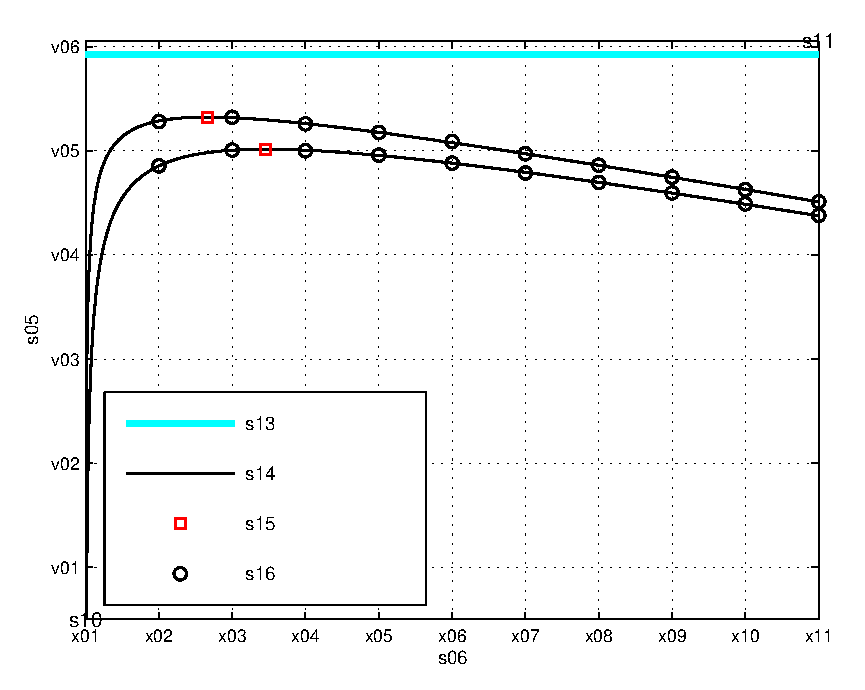
\includegraphics[width= \figscale]{figures/fig_thr_est_time_tradeoff_AWGN}
};
\begin{scope}[x={(image.south east)},y={(image.north west)}]

\draw (0.38,0.78) arc(-130:130:0.005 and 0.015); 
\node[draw, fill=gray!10,font=\footnotesize] at (0.39,0.735) {$\opc = 0.01$};

\draw (0.65,0.77) arc(-130:130:0.005 and 0.015); 
\node[draw,fill=gray!10,font=\footnotesize] at (0.66,0.838) {$\opc = 0.1$};


%\draw[help lines,xstep=.1,ystep=.1] (0,0) grid (1,1);
%\foreach \x in {0,1,...,9} { \node [anchor=north] at (\x/10,0) {0.\x}; }
%\foreach \y in {0,1,...,9} { \node [anchor=east] at (0,\y/10) {0.\y}; }
\end{scope}
\end{tikzpicture}
\caption{Estimation-throughput tradeoff with $\gamma = \SI{0}{dB}$, $\opc \in \{0.01, 0.1\}$ and $\pc = \SI{0}{dBm}$.}
\label{fig:ETT}
%\vspace{-10mm}
\end{figure}
At first, we evaluate the performance of the proposed framework in context to the short-term analysis. \figurename~\ref{fig:Cont_snr} considers the variation of $\preg$ versus $\tau$, refer to Corollary \ref{cor:cor1}. It is depicted that for $\tau \le \SI{0.1}{ms}$, the ST has to control its transmit power ($\preg$), which consequently degrades the link budget for the access channel. 
\figurename~\ref{fig:ETT} analyzes the performance of the US in terms of the estimation-throughput tradeoff, refer to Theorem \ref{th:th1}, corresponding to the Ideal Model (IM) and the proposed Estimation Model (EM). %Clearly, by relaxing the $\opc$, an improvement in performance it terms of $\trs$ is observed. 
It can be depicted that the estimation-throughput tradeoff yields a suitable estimation time $\ttau$ that results in an optimum throughput $\trs(\ttau)$. Hereafter, for the short-term performance analysis, we consider the theoretical expressions and choose to operate at the suitable estimation time. 

\captionsetup[subfigure]{position=top}
\begin{figure*}
%% Add psfrag entries
%\vspace{-5mm}
\centering
\subfloat[]{
\input{figures/fig_opt_thr_vs_SNR_AWGN_SI_00.tex}
\centering
\begin{tikzpicture}[scale=1]
\node[anchor=south west,inner sep=0] (image) at (0,0)
{
	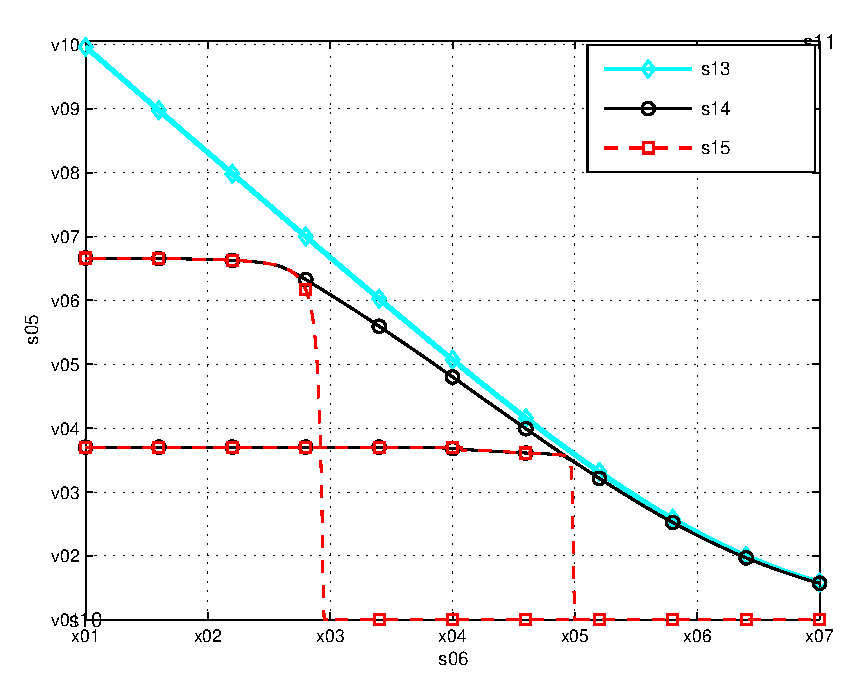
\includegraphics[width= \figscale]{figures/fig_opt_thr_vs_SNR_AWGN_SI_00}
};
\begin{scope}[x={(image.south east)},y={(image.north west)}]

\draw (0.225,0.615) arc(-160:160:0.01 and 0.03);
\node[draw, fill=gray!10, font=\footnotesize] (text1) at (0.7,0.725) {$\pc = \SI{00}{dBm}$};
\draw (0.275,0.33) arc(-160:160:0.01 and 0.03);
\node[draw, fill=gray!10, font=\footnotesize] (text2) at (0.75,0.44) {$\pc = \SI{-10}{dBm}$};
%\draw (0.63,0.66) arc(-150:150:0.016 and 0.048);
\draw[black, ->] (text1.west) -- (0.245,0.635);
%\draw (0.63,0.59) arc(-160:160:0.01 and 0.03);
\draw[black, ->] (text2.west) -- (0.295,0.35);

%\draw[help lines,xstep=.1,ystep=.1] (0,0) grid (1,1);
%\foreach \x in {0,1,...,9} { \node [anchor=north] at (\x/10,0) {0.\x}; }
%\foreach \y in {0,1,...,9} { \node [anchor=east] at (0,\y/10) {0.\y}; }
\end{scope}
\end{tikzpicture}
}
\hfil
\subfloat[]{
\input{figures/fig_opt_thr_vs_SNR_AWGN_SI_10.tex}
\centering
\begin{tikzpicture}[scale=1]
\node[anchor=south west,inner sep=0] (image) at (0,0)
{
	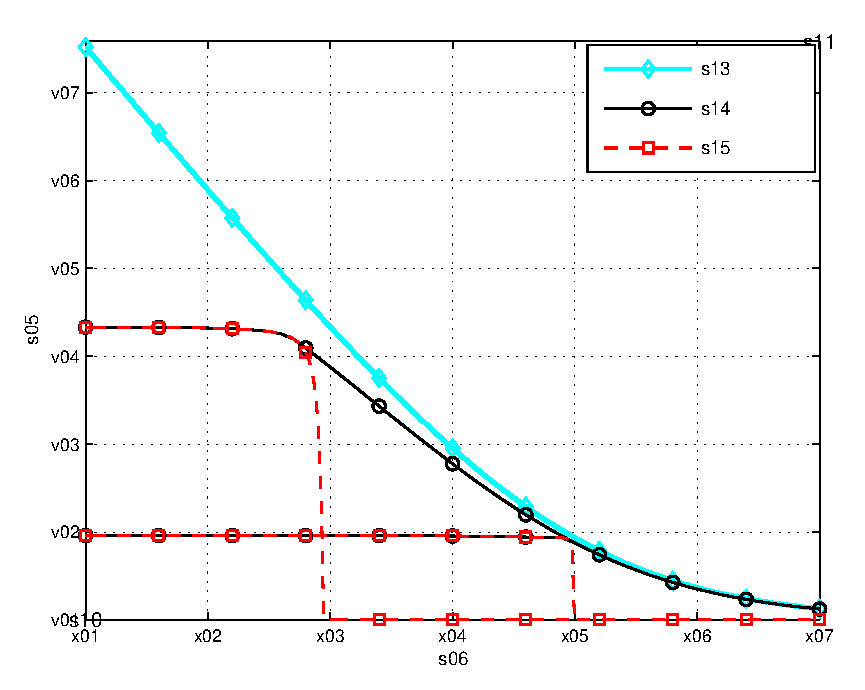
\includegraphics[width= \figscale]{figures/fig_opt_thr_vs_SNR_AWGN_SI_10}
};
\begin{scope}[x={(image.south east)},y={(image.north west)}]

\draw (0.225,0.51) arc(-160:160:0.01 and 0.03);
\node[draw, fill=gray!10, font=\footnotesize] (text1) at (0.7,0.66) {$\pc = \SI{00}{dBm}$};
\draw (0.275,0.2) arc(-160:160:0.01 and 0.03);
\node[draw, fill=gray!10, font=\footnotesize] (text2) at (0.75,0.35) {$\pc = \SI{-10}{dBm}$};
%\draw (0.63,0.66) arc(-150:150:0.016 and 0.048);
\draw[black, ->] (text1.west) -- (0.245,0.53);
%\draw (0.63,0.58) arc(-160:160:0.01 and 0.03);
\draw[black, ->] (text2.west) -- (0.295,0.22);

%\draw[help lines,xstep=.1,ystep=.1] (0,0) grid (1,1);
%\foreach \x in {0,1,...,9} { \node [anchor=north] at (\x/10,0) {0.\x}; }
%\foreach \y in {0,1,...,9} { \node [anchor=east] at (0,\y/10) {0.\y}; }
\end{scope}
\end{tikzpicture}
}
\vspace{4mm}
\caption{Optimum throughput $(\rs(\ttau))$ versus the ratio of the received power to noise $(\gamma)$ with $\opc = 0.1$ and $\pc \in \{-10, 0\} \SI{}{dBm}$ for (a) $\pgpt = \SI{-100}{dBm}$ and (b) $\pgpt = \SI{-90}{dBm}$, which translate to an interference power (from the PT) to noise ratio of (a) $\SI{0}{dB}$ and (b) $\SI{10}{dB}$, respectively, at the SR.}
\label{fig:optT_snr}
%\vspace{-10mm}
\end{figure*}
To procure further insights, the variation of $\trs(\ttau)$ with $\gamma$, where different choices of the secondary interference at the SR (regulated using $\pgpt \in \{-90, -100\} \SI{}{dBm}$) are considered in \figurename~\ref{fig:optT_snr}. It is observed that due to the employed transmit power constraint, $\trs(\ttau)$ gets saturated below a certain $\gamma$, thereby limiting the performance of the US, depicted in Corollary \ref{cor:cor2}. Upon increasing $\pc$ from $\SI{-10}{dB}$ to $\SI{0}{dB}$, the point where saturation is achieved shifts to lower $\gamma$. This is due to the fact that higher $\pc$ extends the operating regime to a lower $\gamma$, consider \figurename~\ref{fig:or}, therefore the secondary system exploits the benefits of operating at a high controlled power because of a low $\gamma$. Particularly for $\pc = \SI{-10}{dBm}$, a severe performance loss indicated by the margin between the IM and the EM is witnessed by the US for $\gamma \le \SI{-2}{dB}$. This signifies that the consideration of the maximum transmit power of the ST is essential while designing the system. Besides this, \figurename~\ref{fig:optT_snr} depicts the performance of the USs with no power control, proposed in Corollary \ref{cor:cor2}. As indicated in \figurename~\ref{fig:or}, beyond a certain $\gamma = \gamma^*$, the USs with no power control delivers no throughput. In order to sustain such situations, the US can exercise power control in order to deliver non-zero throughput. 
%%%%%%%%%%%%%%%%%%%%%%%%%%%%%%%%%%%%%%%%%%%%%%%%%%%%%%%%%%%%%%%%%%%%%%%%%%%%%%%%%%%%%%%%%
\subsection{Long-term analysis} 
%%%%%%%%%%%%%%%%%%%%%%%%%%%%%%%%%%%%%%%%%%%%%%%%%%%%%%%%%%%%%%%%%%%%%%%%%%%%%%%%%%%%%%%%%
Here, we evaluate the performance of the proposed framework, where the interacting channels are under the influence of Nakagami-$m$ fading. For simplification of the analysis, we assume the $m$ parameter to be same for all the involved channels. In addition, we investigate the performance under following fading scenarios: (i) severe fading $m=1$, which corresponds to Rayleigh fading, and (ii) mild fading $m = 5$. First, we analyze the variation of $\preg$ along the estimation time. It is observed that the mild fading scenario ($m = 5$) is more sensitive to the estimation time, see \figurename~\ref{fig:Cont_snr_fad}. Furthermore, comparing the short-term analysis in \figurename~\ref{fig:Cont_snr}, the power control according to the EM saturates with IM at a smaller $\tau$. 

\begin{figure}
%% Add psfrag entries
\input{figures/fig_Preg_est_time_fading.tex}
\centering
\begin{tikzpicture}[scale=1]
\node[anchor=south west,inner sep=0] (image) at (0,0)
{
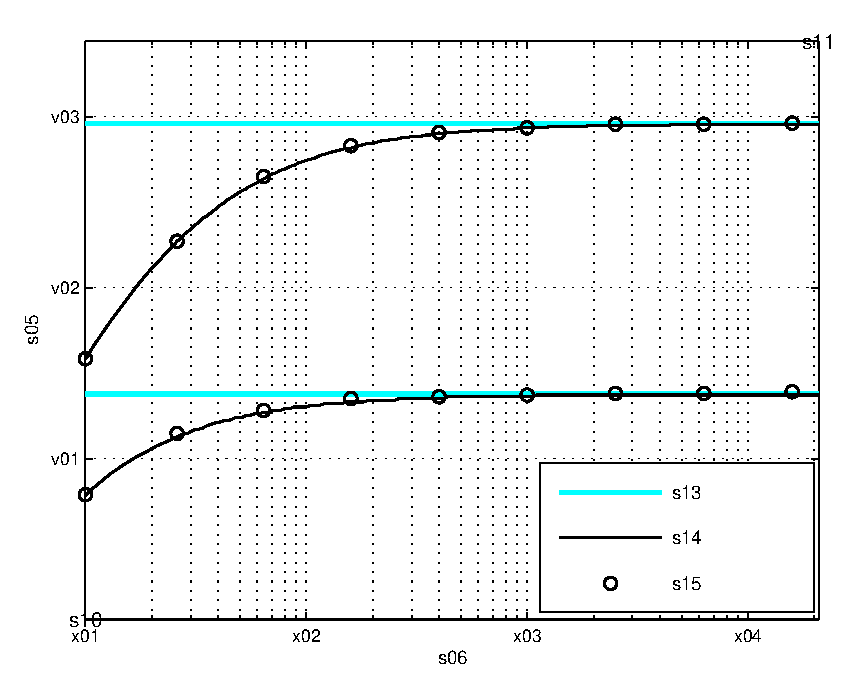
\includegraphics[width= \figscale]{figures/fig_Preg_est_time_fading}
};
\begin{scope}[x={(image.south east)},y={(image.north west)}]

\draw (0.65,0.405) arc(-130:130:0.007 and 0.021);
\node[draw,fill=gray!10,font=\footnotesize] at (0.66,0.365) {$m = 1$};

\draw (0.65,0.815) arc(-130:130:0.007 and 0.021); 
\node[draw,fill=gray!10,font=\footnotesize] at (0.66,0.775) {$m = 5$};

%\draw[black,<->] (0.10,0.87) --  node[above = 0.0mm, font=\footnotesize] {Estimation dominant} (0.535,0.87);
%\draw[black,<->] (0.54,0.87) --  node[above = 0.0mm, font=\footnotesize] {Channel dominant} (0.95,0.87);

%\draw[black,<->] (0.10,0.455) --  node[above = 0.0mm, font=\footnotesize] {Estimation dominant} (0.42,0.455);
%\draw[black,<->] (0.425,0.455) --  node[above = 0.0mm, font=\footnotesize] {Channel dominant} (0.95,0.455);

%\draw[help lines,xstep=.1,ystep=.1] (0,0) grid (1,1);
%\foreach \x in {0,1,...,9} { \node [anchor=north] at (\x/10,0) {0.\x}; }
%\foreach \y in {0,1,...,9} { \node [anchor=east] at (0,\y/10) {0.\y}; }
\end{scope}
\end{tikzpicture}
\caption{Control power versus estimation time with $\gamma = \SI{0}{dB}$, $\opc = 0.1$ and $\pc = \SI{0}{dBm}$ with Nakagami-$m$ fading channel.}
\label{fig:Cont_snr_fad}
\end{figure}

\begin{figure}
%% Add psfrag entries
% This file is generated by the MATLAB m-file laprint.m. It can be included
% into LaTeX documents using the packages graphicx, color and psfrag.
% It is accompanied by a postscript file. A sample LaTeX file is:
%    \documentclass{article}\usepackage{graphicx,color,psfrag}
%    \begin{document}% This file is generated by the MATLAB m-file laprint.m. It can be included
% into LaTeX documents using the packages graphicx, color and psfrag.
% It is accompanied by a postscript file. A sample LaTeX file is:
%    \documentclass{article}\usepackage{graphicx,color,psfrag}
%    \begin{document}% This file is generated by the MATLAB m-file laprint.m. It can be included
% into LaTeX documents using the packages graphicx, color and psfrag.
% It is accompanied by a postscript file. A sample LaTeX file is:
%    \documentclass{article}\usepackage{graphicx,color,psfrag}
%    \begin{document}\input{fig_thr_est_time_tradeoff_fading}\end{document}
% See http://www.mathworks.de/matlabcentral/fileexchange/loadFile.do?objectId=4638
% for recent versions of laprint.m.
%
% created by:           LaPrint version 3.16 (13.9.2004)
% created on:           06-Jan-2016 11:38:21
% eps bounding box:     16 cm x 12 cm
% comment:              
%
%\begin{psfrags}%
%\psfragscanon%
%
% text strings:
\psfrag{s05}[b][b]{\fontsize{8.5}{12.75}\fontseries{m}\mathversion{normal}\fontshape{n}\selectfont \color[rgb]{0,0,0}\setlength{\tabcolsep}{0pt}\begin{tabular}{c}$\rs(\tau)$ [bits/sec/Hz]\end{tabular}}%
\psfrag{s06}[t][t]{\fontsize{8.5}{12.75}\fontseries{m}\mathversion{normal}\fontshape{n}\selectfont \color[rgb]{0,0,0}\setlength{\tabcolsep}{0pt}\begin{tabular}{c}$\tau$ [ms]\end{tabular}}%
\psfrag{s10}[][]{\fontsize{10}{15}\fontseries{m}\mathversion{normal}\fontshape{n}\selectfont \color[rgb]{0,0,0}\setlength{\tabcolsep}{0pt}\begin{tabular}{c} \end{tabular}}%
\psfrag{s11}[][]{\fontsize{10}{15}\fontseries{m}\mathversion{normal}\fontshape{n}\selectfont \color[rgb]{0,0,0}\setlength{\tabcolsep}{0pt}\begin{tabular}{c} \end{tabular}}%
\psfrag{s12}[l][l]{\fontsize{8.5}{12.75}\fontseries{m}\mathversion{normal}\fontshape{n}\selectfont \color[rgb]{0,0,0}Simulated}%
\psfrag{s13}[l][l]{\fontsize{8.5}{12.75}\fontseries{m}\mathversion{normal}\fontshape{n}\selectfont \color[rgb]{0,0,0}IM}%
\psfrag{s14}[l][l]{\fontsize{8.5}{12.75}\fontseries{m}\mathversion{normal}\fontshape{n}\selectfont \color[rgb]{0,0,0}EM}%
\psfrag{s15}[l][l]{\fontsize{8.5}{12.75}\fontseries{m}\mathversion{normal}\fontshape{n}\selectfont \color[rgb]{0,0,0}$\trs(\ttau)$}%
\psfrag{s16}[l][l]{\fontsize{8.5}{12.75}\fontseries{m}\mathversion{normal}\fontshape{n}\selectfont \color[rgb]{0,0,0}Simulated}%
%
% axes font properties:
\fontsize{8.5}{12.75}\fontseries{m}\mathversion{normal}%
\fontshape{n}\selectfont%
%
% xticklabels:
\psfrag{x01}[t][t]{$10^{-2}$}%
\psfrag{x02}[t][t]{$10^{-1}$}%
\psfrag{x03}[t][t]{$10^{0}$}%
\psfrag{x04}[t][t]{$10^{1}$}%
%
% yticklabels:
\psfrag{v01}[r][r]{1}%
\psfrag{v02}[r][r]{1.2}%
\psfrag{v03}[r][r]{1.4}%
\psfrag{v04}[r][r]{1.6}%
\psfrag{v05}[r][r]{1.8}%
\psfrag{v06}[r][r]{2}%
%
% Figure:
%\resizebox{8cm}{!}{\includegraphics{fig_thr_est_time_tradeoff_fading.eps}}%
%\end{psfrags}%
%
% End fig_thr_est_time_tradeoff_fading.tex
\end{document}
% See http://www.mathworks.de/matlabcentral/fileexchange/loadFile.do?objectId=4638
% for recent versions of laprint.m.
%
% created by:           LaPrint version 3.16 (13.9.2004)
% created on:           06-Jan-2016 11:38:21
% eps bounding box:     16 cm x 12 cm
% comment:              
%
%\begin{psfrags}%
%\psfragscanon%
%
% text strings:
\psfrag{s05}[b][b]{\fontsize{8.5}{12.75}\fontseries{m}\mathversion{normal}\fontshape{n}\selectfont \color[rgb]{0,0,0}\setlength{\tabcolsep}{0pt}\begin{tabular}{c}$\rs(\tau)$ [bits/sec/Hz]\end{tabular}}%
\psfrag{s06}[t][t]{\fontsize{8.5}{12.75}\fontseries{m}\mathversion{normal}\fontshape{n}\selectfont \color[rgb]{0,0,0}\setlength{\tabcolsep}{0pt}\begin{tabular}{c}$\tau$ [ms]\end{tabular}}%
\psfrag{s10}[][]{\fontsize{10}{15}\fontseries{m}\mathversion{normal}\fontshape{n}\selectfont \color[rgb]{0,0,0}\setlength{\tabcolsep}{0pt}\begin{tabular}{c} \end{tabular}}%
\psfrag{s11}[][]{\fontsize{10}{15}\fontseries{m}\mathversion{normal}\fontshape{n}\selectfont \color[rgb]{0,0,0}\setlength{\tabcolsep}{0pt}\begin{tabular}{c} \end{tabular}}%
\psfrag{s12}[l][l]{\fontsize{8.5}{12.75}\fontseries{m}\mathversion{normal}\fontshape{n}\selectfont \color[rgb]{0,0,0}Simulated}%
\psfrag{s13}[l][l]{\fontsize{8.5}{12.75}\fontseries{m}\mathversion{normal}\fontshape{n}\selectfont \color[rgb]{0,0,0}IM}%
\psfrag{s14}[l][l]{\fontsize{8.5}{12.75}\fontseries{m}\mathversion{normal}\fontshape{n}\selectfont \color[rgb]{0,0,0}EM}%
\psfrag{s15}[l][l]{\fontsize{8.5}{12.75}\fontseries{m}\mathversion{normal}\fontshape{n}\selectfont \color[rgb]{0,0,0}$\trs(\ttau)$}%
\psfrag{s16}[l][l]{\fontsize{8.5}{12.75}\fontseries{m}\mathversion{normal}\fontshape{n}\selectfont \color[rgb]{0,0,0}Simulated}%
%
% axes font properties:
\fontsize{8.5}{12.75}\fontseries{m}\mathversion{normal}%
\fontshape{n}\selectfont%
%
% xticklabels:
\psfrag{x01}[t][t]{$10^{-2}$}%
\psfrag{x02}[t][t]{$10^{-1}$}%
\psfrag{x03}[t][t]{$10^{0}$}%
\psfrag{x04}[t][t]{$10^{1}$}%
%
% yticklabels:
\psfrag{v01}[r][r]{1}%
\psfrag{v02}[r][r]{1.2}%
\psfrag{v03}[r][r]{1.4}%
\psfrag{v04}[r][r]{1.6}%
\psfrag{v05}[r][r]{1.8}%
\psfrag{v06}[r][r]{2}%
%
% Figure:
%\resizebox{8cm}{!}{\includegraphics{fig_thr_est_time_tradeoff_fading.eps}}%
%\end{psfrags}%
%
% End fig_thr_est_time_tradeoff_fading.tex
\end{document}
% See http://www.mathworks.de/matlabcentral/fileexchange/loadFile.do?objectId=4638
% for recent versions of laprint.m.
%
% created by:           LaPrint version 3.16 (13.9.2004)
% created on:           06-Jan-2016 11:38:21
% eps bounding box:     16 cm x 12 cm
% comment:              
%
%\begin{psfrags}%
%\psfragscanon%
%
% text strings:
\psfrag{s05}[b][b]{\fontsize{8.5}{12.75}\fontseries{m}\mathversion{normal}\fontshape{n}\selectfont \color[rgb]{0,0,0}\setlength{\tabcolsep}{0pt}\begin{tabular}{c}$\rs(\tau)$ [bits/sec/Hz]\end{tabular}}%
\psfrag{s06}[t][t]{\fontsize{8.5}{12.75}\fontseries{m}\mathversion{normal}\fontshape{n}\selectfont \color[rgb]{0,0,0}\setlength{\tabcolsep}{0pt}\begin{tabular}{c}$\tau$ [ms]\end{tabular}}%
\psfrag{s10}[][]{\fontsize{10}{15}\fontseries{m}\mathversion{normal}\fontshape{n}\selectfont \color[rgb]{0,0,0}\setlength{\tabcolsep}{0pt}\begin{tabular}{c} \end{tabular}}%
\psfrag{s11}[][]{\fontsize{10}{15}\fontseries{m}\mathversion{normal}\fontshape{n}\selectfont \color[rgb]{0,0,0}\setlength{\tabcolsep}{0pt}\begin{tabular}{c} \end{tabular}}%
\psfrag{s12}[l][l]{\fontsize{8.5}{12.75}\fontseries{m}\mathversion{normal}\fontshape{n}\selectfont \color[rgb]{0,0,0}Simulated}%
\psfrag{s13}[l][l]{\fontsize{8.5}{12.75}\fontseries{m}\mathversion{normal}\fontshape{n}\selectfont \color[rgb]{0,0,0}IM}%
\psfrag{s14}[l][l]{\fontsize{8.5}{12.75}\fontseries{m}\mathversion{normal}\fontshape{n}\selectfont \color[rgb]{0,0,0}EM}%
\psfrag{s15}[l][l]{\fontsize{8.5}{12.75}\fontseries{m}\mathversion{normal}\fontshape{n}\selectfont \color[rgb]{0,0,0}$\trs(\ttau)$}%
\psfrag{s16}[l][l]{\fontsize{8.5}{12.75}\fontseries{m}\mathversion{normal}\fontshape{n}\selectfont \color[rgb]{0,0,0}Simulated}%
%
% axes font properties:
\fontsize{8.5}{12.75}\fontseries{m}\mathversion{normal}%
\fontshape{n}\selectfont%
%
% xticklabels:
\psfrag{x01}[t][t]{$10^{-2}$}%
\psfrag{x02}[t][t]{$10^{-1}$}%
\psfrag{x03}[t][t]{$10^{0}$}%
\psfrag{x04}[t][t]{$10^{1}$}%
%
% yticklabels:
\psfrag{v01}[r][r]{1}%
\psfrag{v02}[r][r]{1.2}%
\psfrag{v03}[r][r]{1.4}%
\psfrag{v04}[r][r]{1.6}%
\psfrag{v05}[r][r]{1.8}%
\psfrag{v06}[r][r]{2}%
%
% Figure:
%\resizebox{8cm}{!}{\includegraphics{fig_thr_est_time_tradeoff_fading.eps}}%
%\end{psfrags}%
%
% End fig_thr_est_time_tradeoff_fading.tex

\centering
\begin{tikzpicture}[scale=1]
\node[anchor=south west,inner sep=0] (image) at (0,0)
{
\includegraphics[width= \figscale]{figures/fig_thr_est_time_tradeoff_fading}
};
\begin{scope}[x={(image.south east)},y={(image.north west)}]

\draw (0.65,0.445) arc(-130:130:0.007 and 0.021); 
\node[draw,fill=gray!10,font=\footnotesize] at (0.66,0.405) {$m = 1$};

\draw (0.65,0.805) arc(-130:130:0.007 and 0.021); 
\node[draw,fill=gray!10,font=\footnotesize] at (0.66,0.765) {$m = 5$};

\draw[black,<->] (0.10,0.87) --  node[above = 0.0mm, font=\footnotesize] {Estimation dominant} (0.535,0.87);
\draw[black,<->] (0.54,0.87) --  node[above = 0.0mm, font=\footnotesize] {Channel dominant} (0.95,0.87);

\draw[black,<->] (0.10,0.51) --  node[above = 0.0mm, font=\footnotesize] {Estimation dominant} (0.42,0.51);
\draw[black,<->] (0.425,0.51) --  node[above = 0.0mm, font=\footnotesize] {Channel dominant} (0.95,0.51);

%\draw[help lines,xstep=.1,ystep=.1] (0,0) grid (1,1);
%\foreach \x in {0,1,...,9} { \node [anchor=north] at (\x/10,0) {0.\x}; }
%\foreach \y in {0,1,...,9} { \node [anchor=east] at (0,\y/10) {0.\y}; }
\end{scope}
\end{tikzpicture}
\caption{Estimation-throughput tradeoff with $\gamma = \SI{0}{dB}$, $\opc = 0.1$ and $\pc = \SI{0}{dBm}$ with Nakagami-$m$ fading channel. The plot classifies the estimation time into the estimation-dominant and the channel-dominant regime}
\label{fig:ETT_fad}
\end{figure}
To investigate further, the estimation-throughput tradeoff for aforementioned fading scenarios are presented in \figurename~\ref{fig:ETT_fad}, refer to Theorem \ref{th:th2}. Like short-term analysis, It is depicted that for a suitable choice of the estimation time, the performance of the proposed framework that capture imperfect channel knowledge is comparable to the ideal conditions in terms of the achievable secondary throughput. Since the USs are subjected to the variations from the estimation and fading, we classify the estimation time into an estimation-dominant regime and a channel-dominant regime. These regimes signify that the estimation time can only reduce the imperfections (incurred in the USs) due to the channel estimation, however, beyond a certain estimation time ($\ttau$), the time resources allocated for channel estimation slightly contributes to the performance improvement (in terms of the power control, which finally affect the secondary throughput) and largely to the performance degradation (due to the factor $\frac{T - \tau}{T}$ in (\ref{eq:rs_fad})) in the secondary throughput. 
\captionsetup[subfigure]{position=top}
\begin{figure*}
%% Add psfrag entries
%\vspace{-5mm}
\centering
\subfloat[]{
\input{figures/fig_opt_thr_vs_SNR_SI_00_fading.tex}
\centering
\begin{tikzpicture}[scale=1]
\node[anchor=south west,inner sep=0] (image) at (0,0)
{
	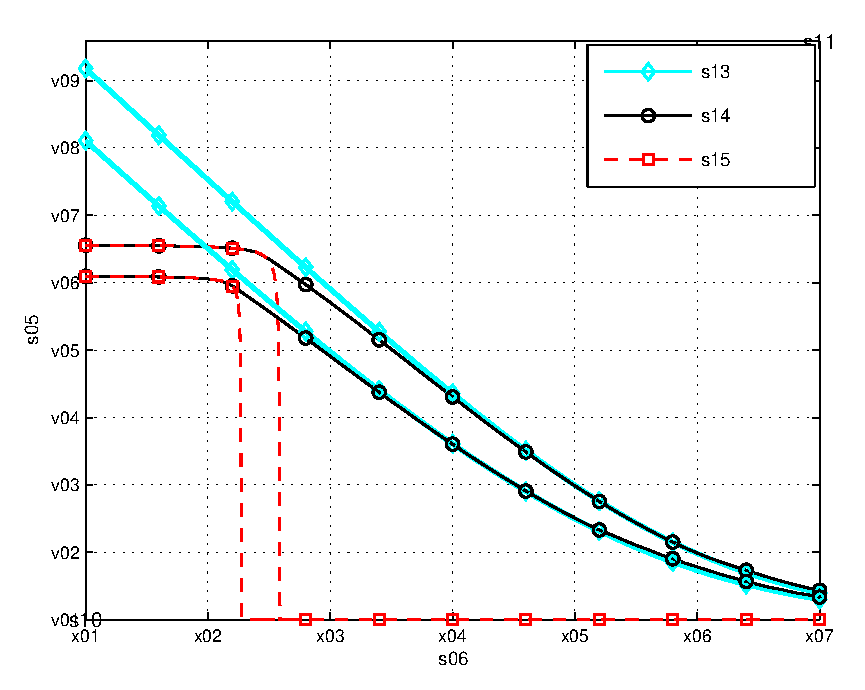
\includegraphics[width= \figscale]{figures/fig_opt_thr_vs_SNR_SI_00_fading}
};
\begin{scope}[x={(image.south east)},y={(image.north west)}]

%\draw (0.125,0.62) arc(-160:160:0.016 and 0.048);
%\node[draw, fill=gray!10, font=\footnotesize] (text1) at (0.2,0.48) {$\pc = \SI{00}{dBm}$};
%\draw[black, ->] (text1.north) -- (0.14,0.59);
%\draw (0.215,0.33) arc(-160:160:0.01 and 0.03);
%\node[draw, fill=gray!10, font=\footnotesize] (text2) at (0.225,0.2) {$\pc = \SI{-10}{dBm}$};
%\draw[black, ->] (text2.north) -- (0.225,0.31);


\draw (0.4,0.54) arc(-160:160:0.007 and 0.021);
\node[draw, fill=gray!10, font=\footnotesize] (text3) at (0.55,0.7) {$m = 5$};
\draw[black, ->] (text3.south) -- (0.412,0.562);

\draw (0.43,0.43) arc(-160:160:0.007 and 0.021);
\node[draw, fill=gray!10, font=\footnotesize] (text4) at (0.58,0.58) {$m = 1$};
\draw[black, ->] (text4.south) -- (0.442,0.452);

%\draw[help lines,xstep=.1,ystep=.1] (0,0) grid (1,1);
%\foreach \x in {0,1,...,9} { \node [anchor=north] at (\x/10,0) {0.\x}; }
%\foreach \y in {0,1,...,9} { \node [anchor=east] at (0,\y/10) {0.\y}; }
\end{scope}
\end{tikzpicture}
}
\hfil
\subfloat[]{
\input{figures/fig_opt_thr_vs_SNR_SI_10_fading.tex}
\centering
\begin{tikzpicture}[scale=1]
\node[anchor=south west,inner sep=0] (image) at (0,0)
{
	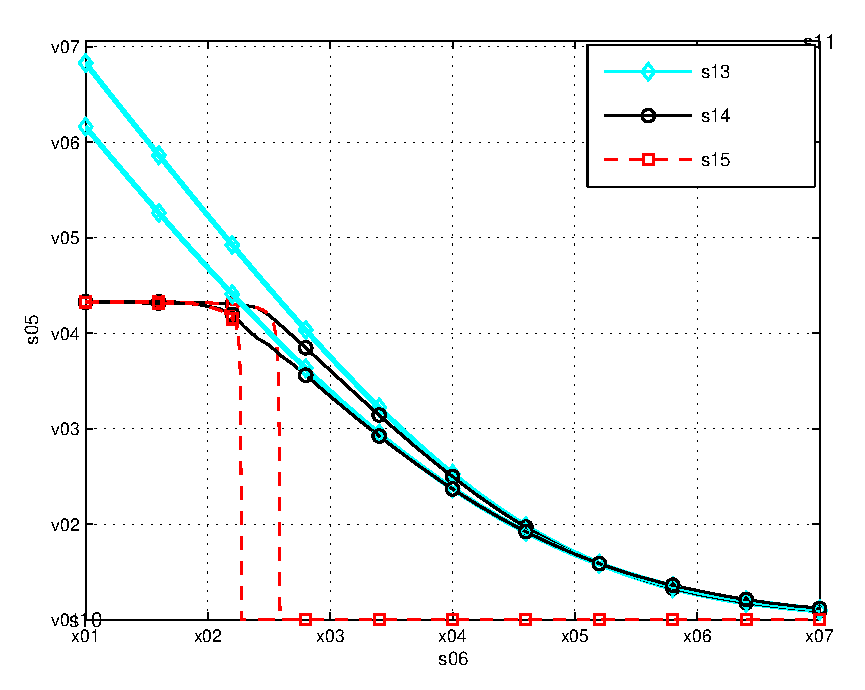
\includegraphics[width= \figscale]{figures/fig_opt_thr_vs_SNR_SI_10_fading}
};
\begin{scope}[x={(image.south east)},y={(image.north west)}]

%\draw (0.125,0.565) arc(-160:160:0.01 and 0.03);
%\node[draw, fill=gray!10, font=\footnotesize] (text1) at (0.2,0.42) {$\pc = \SI{00}{dBm}$};
%\draw[black, ->] (text1.north) -- (0.142,0.557);
%\draw (0.215,0.235) arc(-160:160:0.01 and 0.03);
%\node[draw, fill=gray!10, font=\footnotesize] (text2) at (0.225,0.175) {$\pc = \SI{-10}{dBm}$};
%\draw[black, ->] (text2.north) -- (0.225,0.21);


\draw (0.4,0.435) arc(-160:160:0.007 and 0.021);
\node[draw, fill=gray!10, font=\footnotesize] (text3) at (0.55,0.585) {$m = 5$};
\draw[black, ->] (text3.south) -- (0.412,0.457);

\draw (0.462,0.325) arc(-160:160:0.007 and 0.021);
\node[draw, fill=gray!10, font=\footnotesize] (text4) at (0.38,0.3) {$m = 1$};
\draw[black, ->] (text4.east) -- (0.462,0.32);

%\draw[help lines,xstep=.1,ystep=.1] (0,0) grid (1,1);
%\foreach \x in {0,1,...,9} { \node [anchor=north] at (\x/10,0) {0.\x}; }
%\foreach \y in {0,1,...,9} { \node [anchor=east] at (0,\y/10) {0.\y}; }
\end{scope}
\end{tikzpicture}
}
\vspace{4mm}
\caption{Optimum throughput $(\rs(\ttau))$ versus the ratio of the received power to noise $(\gamma)$ for Nakagmi-$m$ fading channels with $\opc = 0.1$ and $\pc = 0$ \SI{}{dBm} for (a) $\pgpt = \SI{-100}{dBm}$ and (b) $\pgpt = \SI{-90}{dBm}$, which correspond to an interference power (from the PT) to noise ratio of (a) $\SI{0}{dB}$ and (b) $\SI{10}{dB}$, respectively, at the SR.}
\label{fig:optT_snr_fad}
%\vspace{-10mm}
\end{figure*}

Upon determining the optimum secondary throughput $(\rs(\ttau))$ using the estimation-throughput tradeoff, we consider the variation of the $\rs(\ttau)$ along the received signal to noise ratio for different choices of the secondary interference in \figurename~\ref{fig:optT_snr_fad}. It is observed that for a large range ($\gamma \ge \SI{-10}{dB}$), the optimum secondary throughput determined by the EM closely follows the throughput depicted by the IM. In addition, \figurename~\ref{fig:optT_snr_fad} considers the performance of the USs with no power control, refer to Corollary \ref{cor:cor3}. Following the discussion in Remark \ref{rm:rm2}, it was indicated the performance limit ($\gamma^*$) shifts to a lower $\gamma$ when fading becomes severe, refer to \figurename~\ref{fig:or_fad}. This effect is finally translated to the secondary throughput, where $m = 1$ approaches the region with no throughput at a lower $\gamma$ as compared to $m = 5$, consider \figurename~\ref{fig:optT_snr_fad}. 
\section{Conclusion} \label{sec:conc}
%%%%%%%%%%%%%%%%%%%%%%%%%%%%%%%%%%%%%%%%%%%%%%%%%%%%%%%%%%%%%%%%%%%%%%%%%%%%%%%%%%%%%%%%%
In this paper, we studied the performance of the USs from a deployment perspective. In this view, a novel approach that incorporates channel estimation has been proposed. To capture the impact of the imperfect channel knowledge, an outage constraint that precludes the performance degradation by regulating the excessive interference in terms of interference power received at the primary receiver has been employed. With the inclusion of a transmit power constraint, the operating and the non-operating regimes that classify the performance limit for the US have been established. Further, a power control mechanism subject to the outage and the transmit power constraints has been proposed. Finally, the estimation-throughput tradeoff has been investigated to determine the achievable secondary throughput for the US. %In future work, we plan to extend the proposed analysis to include the effect of channel fading in order to characterize the long-term performance of the USs. 
In future work, we plan to extend the proposed analysis to capture the influence of other primary and secondary users in the network on the performance of the underlay systems. 
%%%%%%%%%%%%%%%%%%%%%%%%%%%%%%%%%%%%%%%%%%%%%%%%%%%%%%%%%%%%%%%%%%%%%%%%%%%%%%%%%%%%%%%%%
%\appendix[Proof of Lemma 5] \label{ap:one}
%%%%%%%%%%%%%%%%%%%%%%%%%%%%%%%%%%%%%%%%%%%%%%%%%%%%%%%%%%%%%%%%%%%%%%%%%%%%%%%%%%%%%%%%%
\begin{IEEEproof}
For simplification, we break the expression $\frac{\epgs \ptran}{\eprcvdsr}$ and determine the pdf for $f_{\epgs \ptran}$ and $f_{\eprcvd}$ separately.
Using (\ref{eq:fehs}) in Lemma \ref{lm:lm2}, the pdf of $f_{\epgs \ptran}$ is determined as
\begin{align}
f_{\epgs \ptran}(x) = \frac{1}{\Gamma(\as) (\bs \ptran)^{\as}} x^{\as - 1} \exp\left( - \frac{x}{ \bs \ptran} \right), \label{eq:step1} 
\end{align}
where $\as$ and $\bs$ are defined in (\ref{eq:para_s}).
Similarly, using Lemma \ref{lm:lm3}, the pdf of $f_{\eprcvdsr}$ is characterized as
\begin{align}
f_{\eprcvd}(x) = \frac{1}{\Gamma(\apt) (\bpt)^{\apt}} x^{\apt - 1} \exp\left( - \frac{x}{ \bpt} \right), \label{eq:step2} 
\end{align}
where $\apt$ and $\bpt$ are defined in (\ref{eq:para_pt}).

Using (\ref{eq:step1}) and (\ref{eq:step2}), we apply Mellin transform \cite{NIST} to determine the pdf of $\frac{\epgs \ptran}{\eprcvdsr}$ as
\begin{align}
f_{\frac{\epgs \ptran}{\eprcvdsr}}(x) = \frac{(x)^{\as - 1} \Gamma(\as + \apt)}{\Gamma(\as) \Gamma(\apt) (\bs \ptran) ^{\as} \bpt^{\apt}} \left(\frac{1}{\bpt} + \frac{x - 1}{\bs \ptran}\right).
\end{align}
Finally, substituting the expression $\frac{\epgs \ptran}{\eprcvdsr}$ in $\ca$ yields (\ref{eq:den_C}).
\end{IEEEproof}


%\section{Introduction}
%\subsection{Power control}
%Transmission power control

%\section{Performance characterization}
%\begin{figure}[!t]
%	\centering
%     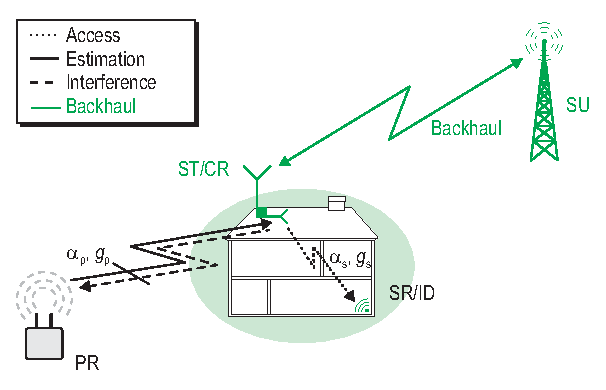
\includegraphics[trim=0cm 0.0cm 0.0cm 0cm,clip=true,width=0.8\columnwidth]{figures/CR_Scenario_Underlay}
%\caption{An illustration of a single \ac{CR} underlay scenario}
%\label{fig:Und_Sc}
%\end{figure}

%\subsection{Estimation-Throughput Tradeoff}
%\subsection{Perfect channel estimation}
%\begin{itemize}
%\item Unknown received power
%\item Noise uncertainty
%\end{itemize}

%\begin{figure}[!t]
%	\centering
%        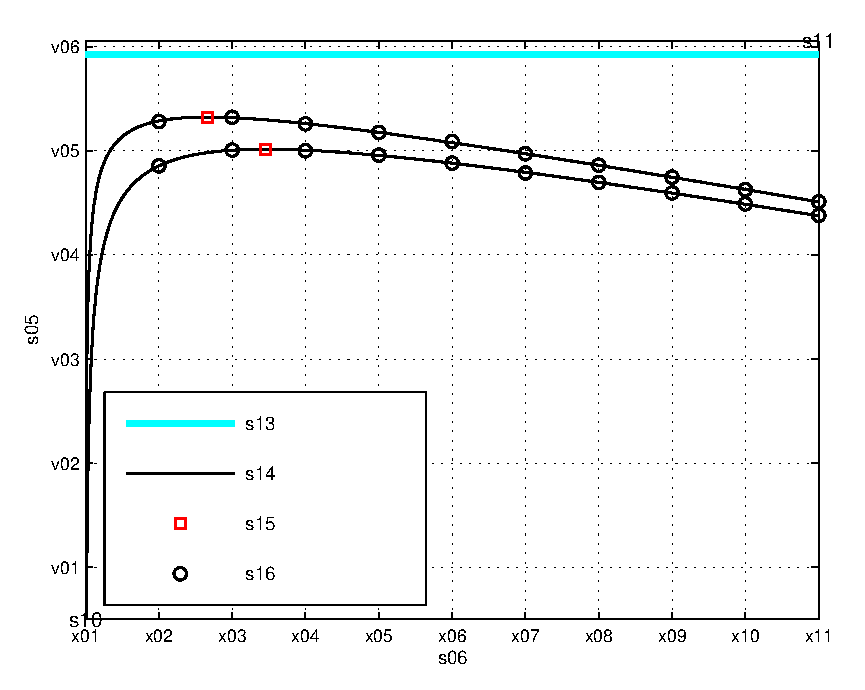
\includegraphics[width=0.8\columnwidth]{figures/fig_thr_est_time_tradeoff_AWGN}
%	\caption{An illustration of estimation-throughput tradeoff}
%	\label{fig:ID_OC}
%\end{figure}



%\section{Cognitive relay networks}
%\subsection{System model}

%\begin{figure}[!t]
%        \centering
%        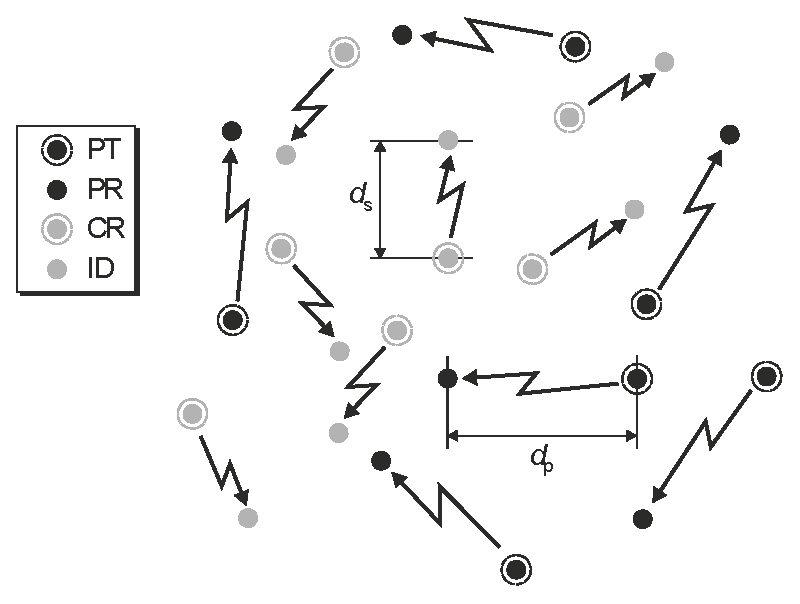
\includegraphics[trim=0.0cm 0.0cm 0.0cm 0.0cm,clip=true,width=0.8\columnwidth]{figures/SGeometry}
%        \caption{A realization of a PPP for a cognitive relay network, depicting interference among the primary and secondary nodes.} 
%        \label{fig:Int_Sc}
%\end{figure}
%\cite{Kaushik_PIMRC}

%
%\section{Overview of the TETRA standard}
%\ac{TETRA}\index{TETRA} is an open specification for a digital communication system defined by \ac{ETSI} in 1995. It is intended as a radio link for public safety agencies like police or fire department and will replace legacy analog radio devices. Therefore, the carrier frequency was specified to be in the already existing VHF and UHF bands for \ac{PMR}\index{Public Mobile Radio}. With a bandwidth of \SI{25}{kHz}, two \SI{12.5}{kHz} wide analog FM channels can be replaced by one channel of the new digital system. Due to the TDMA structure with four time slots per channel, the number of users for each channel can be doubled. Furthermore, new features like multicasting and broadcasting, data transmission and encryption, access to the Internet and a better resistance against interferences are added. Although its first draft was released in 1995, the integration of the system in the current radio communication structure for public mobile radio is still ongoing. The European project WINTSEC proposed \ac{SDR} as a way for cost efficient introduction of new communication systems by a software based interoperability with the legacy devices.
%
%This chapter describes the software based development of a TETRA waveform under the aspect of portability. Due to the high complexity of the specification, this work focuses on the user plane of the \ac{V+D} air interface protocol stack. Therefore, \ac{PHY} and \ac{MAC} layers are implemented. For completeness, figure \ref{fig:architecture_VD} shows the architecture of the \ac{V+D} protocol stack for the user plane as well as the higher levels of the control plane. The implemented \ac{PHY} and \ac{MAC} layers are highlighted in gray.
%
%\begin{figure}[htb]
%	\centering
%		\includegraphics[]{../kapitel04/figures/architecture_VD.pdf}
%	\caption{Architecture of the V+D protocol stack, based on \cite{Steppler}}
%	\label{fig:architecture_VD}
%\end{figure}
%
%The user plane specifies four possible traffic channels for transmitting user data, which are distinguished according to the robustness of channel coding and the data rate as follows\index{Traffic channel}:
%		\begin{description}
% 	 		\item [Traffic CHannel/2.4 (TCH/2.4):]
%				Channel for data transmission with high protection. The bit rate is according to the name \SI{2.4}{kbit/s}
%
% 	 		\item [Traffic CHannel/4.8 (TCH/4.8):]
%				Channel for data transmission with low protection. The bit rate is according to the name \SI{4.8}{kbit/s}
%			
%			\item [Traffic CHannel/7.2 (TCH/7.2):]
% 				Channel for data transmission without protection. The bit rate is according to the name \SI{7.2}{kbit/s}
%
%			\item [Traffic CHannel/Speech (TCH/S):]
%			  Channel for speech transmission, due to the bit rate of the underlying voice codec of \SI{4567}{bit/s}, the TCH/S uses TCH/4.8.
%		\end{description}
%The various traffic channels described above are only logical channels. The mapping from logical to physical channels will be described in the specification of the \ac{PHY} in section \ref{sec:cim_phy}.
%		
%\section{Computational Independent Model}
%\label{sec:TETRA_CIM}
%\index{CIM}
%\subsection{Media Access Control}
%\index{Media Access Control}
%The \ac{MAC} layer of TETRA consists of channel coding\index{Channel coding}, interleaving\index{Interleaving} and scrambling\index{Scrambling} according to figure \ref{fig:architecture_VD}. These operations are shown in more detail in figure \ref{fig:MAC_TETRA} with separation in the different traffic channels. For a complete description of the individual coding and interleaving schemes, five planes are introduced that separate the different processing blocks. In this nomenclature $b_x[k]$ is the bit at position $k$ of plane number $x$. The figure shows furthermore the width of the bit fields, which differs according to the data rate of the different channels. The length of these fields in plane $x$ is named $K_x$. 
%
%\begin{figure}[htb]
%	\centering
%		\includegraphics[]{../kapitel04/figures/MAC_TETRA.pdf}
%	\caption{Overview of the encoding and scrambling schemes, used in the transmit side of the traffic channel}
%	\label{fig:MAC_TETRA}
%\end{figure}
%
%To assure that the convolutional encoder ends up in a defined state, the information bits for TCH/2.4 and TCH/4.8 must be extended with four tail bits according to the following clauses:
%
%\begin{equation}
% b_2[k]= 
%\begin{cases}
%	b_1[k] & \text{for} \quad 1 \leq k \leq K_1 \\
%	0			 & \text{for} \quad K_1 < k \leq K_2
%	\end{cases}
%\end{equation}
%
%For the TCH/2.4 the length of the vector is $K_1=144$ while for the TCH/4.8 the length is specified to $K_1=288$. For these channels a zero padding of four bits is inserted due to the register length of four for the following encoding. Therefore, the length of $K_2$ can be determined to be $K_2 = K_1+4$. Due to the fact that the  TCH/7.2 is not protecting its information with channel encoding, neither tail bits nor encoding schemes or interleaving are needed. For the traffic channels TCH/2.4 and TCH/4.8 the convolutional coding is identical. The encoded bits $b_3$ can be calculated by:
%
%\begin{equation}
% b_3[4(k-1)+i]=\sum_{j=0}^{4} b_2[k-j]g_{i,j} \quad \text{for} \quad 
%\begin{cases}
%             &i=1, 2, 3, 4    \\
%             &k=1, 2,..., K_2 \; .
% \end{cases}
%\end{equation}
%
%In this equation, $g_{i,j}$ is the element $j$ at row $i$ of the matrix that can be described by the generator polynomials of the rate $\frac{1}{4}$ mother code:
%
%\begin{table}[!!ht]
%	\centering\begin{tabular}{lcl}
%		$G_1(X)=1+X+X^4$		&$\Rightarrow$	&$g_1=[1 1 0 0 1]$\\
%		$G_2(X)=1+X^2+X^3+X^4$	&$\Rightarrow$	&$g_2=[1 0 1 1 1]$\\
%		$G_3(X)=1+X+X^2+X^4$	&$\Rightarrow$	&$g_3=[1 1 1 0 1]$\\
%		$G_4(X)=1+X+X^3+X^4$	&$\Rightarrow$	&$g_4=[1 1 0 1 1]$\\
%	\end{tabular}\\
%\end{table}
%
%At this point, the traffic channels have different frame lengths. This can also be seen in figure \ref{fig:MAC_TETRA}. The length of the bit field $K_3$ is 592 for the TCH/2.4, 1168 for the TCH/4.8 and 432 for the TCH/7.2. To achieve the specified frame length of $K_4 = 432$ bit, which is equal for all channels, the redundancy of the encoded channels is reduced with different puncturing schemes. The puncturing\index{Puncturing} can be described as follows:
%\begin{equation}
%b_4[k] = b_3[j(k)]
%\label{eq:pun}
%\end{equation}
%
%The index $j$ can be calculated dependent on the index $k$ from the output vector by the following equation for the TCH/2.4: 
%
%\begin{equation}
%	j(k) = 8\left(\left\lfloor \frac{k-1+k_{35}}{6}\right\rfloor \right)+ P_{2.4} \left( k+k_{35} - 6 \cdot \left\lfloor \frac{k-1+k_{35}}{6}\right\rfloor\right),
%\end{equation}
%
%where $\lfloor x \rfloor$ is the floor function\index{Floor function} that rounds down to the largest integer smaller than $x$. The variable $k_x$ is a counter that increments for multiples of $x$. This can be described by
%\begin{equation}
%k_x = \left\lfloor \frac{k-1}{x}\right\rfloor.
%\end{equation}
%
%The mapping of $P_{2.4}$ is depicted in table \ref{tab:Punct_TCH}. For the TCH/4.8 the index $j$ is calculated with
%\begin{equation}
%	j(k) = 8\left(\left\lfloor \frac{k-1+k_{65}}{3}\right\rfloor \right) + P_{4.8} \left( k+k_{65} - 3 \cdot \left\lfloor \frac{k-1+k_{65}}{3}\right\rfloor\right),
%\end{equation}
%
%where the mapping of $P_{4.8}$ is also depicted in table \ref{tab:Punct_TCH}.
%
%\begin{table}[h]
%	\centering
%		\begin{tabular}{c|c|c}
%		\toprule
%			$i$ & $P_{2.4}(i)$ & $P_{4.8}(i)$ \\
%		\midrule
%			1 & 1			& 1 \\
%			2 & 2			& 2 \\
%			3 & 3			& 5 \\
%			4 &	5			&   \\
%			5 &	6			&   \\
%			6 &	7			&   \\
%			\bottomrule
%		\end{tabular}
%		\caption{Mapping of the puncturing scheme for TCH/2.4 and TCH/4.8}
%		\label{tab:Punct_TCH}
%\end{table}
%
%The interleaving mechanism follows the same rule for TCH/2.4 and TCH/4.8 respectively. Therefore the bits are interleaved by
%\begin{equation}
%b_5[k] = b_4\left[ 1+ \left((103 \cdot k) \bmod (432) \right )  \right] \quad \text{for} \quad 1 \leq k \leq 432 \;.
%\label{eq:int_tx}
%\end{equation}
%
%While interleaving is only applied within the convolutional encoded channels, the scrambling mechanism is the same for all traffic channels. It is done by adding a pseudo noise sequence $p[k]$ to the bits:
%\begin{equation}
%b_6[k] = b_5[k] \oplus p[k] \quad \text{for} \quad 1 \leq k \leq 432
%\end{equation}
%
%The scrambling sequence $p[k]$ is generated by a 32 bit wide linear feedback shift register with a connection polynomial of
%
%\begin{eqnarray*}
%c(x) 	&=& \sum_{i=0}^{32}{c_i x^i}\\
%			&=& 1+x+x^2+x^4+x^5+x^7+x^8+x^{10} \\
%			& & +x^{11}+x^{12}+x^{16}+x^{22}+x^{23}+x^{26}+x^{32} \;.
%\end{eqnarray*}
%
%Hereby, the $k$-th bit of the scrambling sequence is given by
%\begin{equation}
%p[k] = \sum_{i=1}^{32}c_i p[k-i].
%\end{equation}
%
%Beside the connection polynomial, the initialization of the register defines the scrambling code. This is done with the \textsc{Extended Colour Code}\index{Extended Colour Code} $e[k]$:
%\begin{equation}
%p[k] = \begin{cases}
%e[1-k]  & \quad \text{for} \quad -29 \leq k \leq 0 \\
%1				& \quad \text{for} \quad -31 \leq k \leq -30 \\
%\end{cases}
%\end{equation}
%The \textsc{Extended Colour Code} consists of 30 bits and describes the mobile station according to figure \ref{fig:ECC}. The first ten bits are defined by the \textsc{Mobile Country Code} which identifies the country where the device is registered. The next 14 bits identify the access net within the country with the \textsc{Mobile Network Code}. The last six bits, finally, represent the \textsc{Colour Code}, which identifies the individual mobile \cite{DigCom_tetra}. To achieve a register length of 32, two defined bits are added.
%
%\begin{figure}[htb]
%	\centering
%		\includegraphics[]{../kapitel04/figures/Extended_Colour_Code.pdf}
%	\caption{Initialization of the scrambling registers with the \textsc{Extended Colour Code}}
%	\label{fig:ECC}
%\end{figure}
%
%
%\subsection{Physical Layer}
%\label{sec:cim_phy}
%\index{Physical layer}
%
%Similar to the well known \ac{GSM} standard, \ac{TETRA} is specified to use a combination of \ac{TDMA} and \ac{FDMA} to give multiple users access to the air interface. A \ac{TDMA} frame in the TETRA system consists of four time slots, for supporting up to four users on a single frequency of \SI{25}{kHz} bandwidth. Uplink and downlink are separated in time and frequency where the various European regulatory organizations agreed on a distance of \SI{10}{MHz} between uplink and downlink carrier. To ease the requirements for a mobile station, uplink and downlink are not only separated in frequency, they are further shifted by two slots in time. Figure \ref{fig:physical_channel} shows the \ac{TDMA}/\ac{FDMA} structure with the combination of \ac{FDD} and \ac{TDD}. The gray boxes show an example of a physical channel, defined with a pair of frequencies (for uplink and downlink carriers) and a corresponding time slot number \cite{ETSI07}. 
%
%\begin{figure}[htb]
%	\centering
%		\includegraphics[]{../kapitel04/figures/physical_channel.pdf}
%	\caption{Overview of the FDMA/TDMA structure}
%	\label{fig:physical_channel}
%\end{figure}
%
%In every occupied time slot one burst is transmitted. TETRA specifies four bursts for the downlink and another three bursts for the uplink. With these bursts, control information, synchronization mechanisms and user data can be transmitted. Due to the fact that this work is focused on the user plane, only the bursts containing user data or synchronization information are considered. A \textsc{Normal Uplink Burst} or a \textsc{Normal Downlink Burst} consists of 510 bits and maps the logical traffic channels to the physical channels by extending the coded bits with training sequences, guard intervals and control information. In addition, special synchronization bursts ensure that the mobile station can be synchronized to its frequency and frame structure. Examples of uplink and downlink bursts, specified in the TETRA standard and considered in the \ac{CIM}, are shown in figure \ref{fig:TETRA_bursts}. To achieve a data transmission, the \textsc{Normal Downlink Burst}\index{Normal Downlink Burst} is transmitted. The two blocks with encoded data comprise of the 432 bit long traffic channel, which can be encoded with the error schemes described in the previous section. The broadcast bits, indicated as BBK in figure \ref{fig:TETRA_bursts}, are control information from the \ac{AACH}\index{Access Assignment Channel}. This is a channel that controls the time slot occupation in uplink and downlink. As mentioned previously, this work focuses on the user plane. However, for the sake of completeness the \ac{AACH} is part of the \textsc{Normal Downlink Burst} and has therefore to be implemented. The information for the \ac{AACH} consists of 14 bits that are encoded with a shortened Reed Muller code\index{Reed Muller code}, leading to a coded bit length of 30. The generator matrix can be found in \cite{ETSI07}. The coded bits are scrambled with the scheme described above and form the BBK bits in the \textsc{Normal Downlink Burst}.
%
%
%\begin{figure}[htb]
%	\centering
%		\includegraphics[]{../kapitel04/figures/TETRA_bursts.pdf}
%	\caption{TETRA V+D uplink and downlink burst types}
%	\label{fig:TETRA_bursts}
%\end{figure}
%
%The bits of the bursts are modulated with a \ac{DQPSK}\index{Phase-Shift keying} scheme with a phase offset of $\nicefrac{\pi}{4}$. Due to the fact that a phase rotation must occur between two adjacent symbols, the current symbol $s[k]$ can be calculated dependent on the previous one by
%
%\begin{equation}
%		s[k]=s[k-1]e^{j\phi[k]} \quad \text{with} \quad s[0]=1\;.
%\end{equation}
%
%The phase offset $\phi[k]$ depends on the current symbol and can be determined using table \ref{table:phase_offset}. With these values, no phase shift of $\pm \pi$ occurs, which reduces fluctuations in the magnitude of the complex envelope. This eases the linearization requirements of power amplifiers, especially in mobile devices where power amplifier should be as cheap as possible. The signal trajectory of this modulation scheme is shown on the left hand side in figure \ref{fig:sig_const}. Another advantage of this modulation scheme is that it allows non-coherent demodulation at the receiver, due to the fact that information is not transmitted with the current phase but with the phase offset. Even if the \ac{SNR}\index{Signal-to-Noise Ratio} has to be doubled to achieve the same bit error rate as QPSK, the ease of the synchronization compensates this loss.
%
%\begin{table}[htb]
%\captionabove{Phase offset depending on the actual symbol}\label{table:phase_offset}
%	\centering\begin{tabular}{cc|c|c}
%	\toprule
%	Bit 2	& Bit 1	& Symbol	& $\phi$[k] \\
%	\midrule
%	$1$	& $1$	& $3$	& - $\frac{3\pi}{4}$  \\
%	$0$	& $1$	& $1$	& + $\frac{3\pi}{4}$  \\
%	$0$	& $0$	& $0$	& - $\frac{\pi}{4}$  \\
%	$1$	& $0$	& $2$	& + $\frac{\pi}{4}$  \\
%	\bottomrule
%	\end{tabular}
%\end{table}
%
%To generate the transmit signal $s_\text{tx}(t)$, the discrete time symbols $s[k]$ are filtered with a time continuous pulse shaping\index{Pulse shaping} filter $g_{\text{RRC}}(t)$. This can be described as follows: 
%
%\begin{equation}
%		s_\text{tx}(t)=\sum_{k=0}^{K}{s[k] \cdot g_{\text{RRC}}(t-kT_\text{sym})},
%\end{equation}
%
%where $T_\text{sym}$ is the symbol duration of \SI{55.56}{\micro s} and $K$ is the maximum number of symbols. The impulse response of the pulse shaping filter $g_{\text{RRC}}(t)$ is obtained by the inverse Fourier transform of a square root raised cosine\index{Root raised cosine} spectrum $G_{\text{RRC}}(f)$ with roll-off factor $\alpha$  defined as
%\begin{align}	
%G_{\text{RRC}}(f)=
%\begin{cases} 
%1,     & |f| \leq \frac{1-\alpha}{2T_{\text{sym}}} \\
%\cos \left(\frac{\pi T_{\text{sym}}}{2 \alpha}\left( |f| - \frac{1 - \alpha}{2 T_{\text{sym}}}\right)\right), 
%      & \frac{1-\alpha}{2T_{\text{sym}}} < |f| \leq \frac{1+\alpha}{2T_{\text{sym}}} \\
%0,     & |f| > \frac{1+\alpha}{2T_{\text{sym}}}\;.
%\end{cases}
%\label{eq:g_rrc_f}
%\end{align}
%
%TETRA specifies $\alpha = 0.35$ and offers the possibility to implement a time limited version of $g_\text{RRC}(t)$ that fulfills the constraints of modulation accuracy and adjacent channel attenuation. Therefore, the sequence of  complex symbols $s[k]$ must be interpolated by a factor of $I_\text{RRC}$ and furthermore filtered with a discrete time realization of the root raised cosine filter. This is identical to the sampling of the time continuous transmit function $s_\text{tx}(t)$ with sampling rate $I_\text{RRC}/T_\text{sym}$. Hence, the discrete time signal of the transmit sequence can be described as
%
%\begin{equation}
%s_\text{tx}\left(i \cdot \frac{T_\text{sym}}{I_\text{RRC}}\right)  = \sum_{k=0}^{K}{s[k]g_{\text{RRC}}\left(i \cdot \frac{T_\text{sym}}{I_\text{RRC}}-kT_\text{sym}\right)}\;.
%\end{equation}
%
%The design of the filter $g_\text{RRC}(\cdot)$ is platform specific due to the sample rate conversion. Therefore it is part of the \ac{PSM}. However, it has to be mentioned that the pulse shaping filter results in larger fluctuations of the complex envelope and hence a smaller hole of the signal trajectory in the complex plane. This effect is shown on the right hand side of figure \ref{fig:sig_const}.
%
%\begin{figure}[htb]
%	\centering
%		\includegraphics[width=1.00\textwidth]{../kapitel04/figures/sig_const.pdf}
%	\caption{Signal trajectory of the $\frac{\pi}{4}$-DQPSK modulation scheme}
%	\label{fig:sig_const}
%\end{figure}
%
%Table \ref{table:TETRA_overview} summarizes the key parameters of the TETRA system.
%
%\begin{table}[htb]
%\captionabove{Overview of the TETRA system parameter}\label{table:TETRA_overview}
%	\centering\begin{tabular}{cccc}
%	\toprule
%	Parameter					& Value \\
%	\midrule
%	Carrier frequency	& 400 MHz	 \\
%	Bandwidth					& 25 kHz \\
%	Media access			& TDMA/FDMA \\
%	Duplex mode				& TDD/FDD \\
%	Users per carrier	& 4 \\
%	Modulation				& $\frac{\pi}{4}$-DQPSK \\
%	Channel coding		& RCPC \\
%	Symbol rate				& 18 kBaud/s \\
%	Bits per slot			& 510 \\
%	Frame duration		& 56.67 ms \\
%	Bursts per frame	& 4 \\
%	Burst duration		& 14.167 ms \\
%	Pulse shaping			& RRC with 0.35 rolloff \\
%	Data rate					& up to 28.8 kbit/s \\
%	\bottomrule
%	\end{tabular}
%\end{table}
%
%\section{Platform Independent Model}
%\index{CIM}
%\label{sec:PIM_TETRA}
%The Platform Independent Model of TETRA is the implementation of the transmit path as described in the \ac{CIM} in the previous section \ref{sec:TETRA_CIM}. Furthermore, the receive side is implemented with the synchronization of time, frequency and frame, which is not described in the \ac{CIM}.
%
%\subsection{Transmitter}
%The input of the transmitter is a vector with random bits generated by a \ac{PN} sequence and is used as information data. The length of this array depends on the traffic channel and can vary from 144 bits for the TCH/2.4, over 288 bits for the TCH/4.8 to 432 bits for the TCH/7.2. The encoding depends also on the traffic channel and assures an output length of 432 bits, independent of the channel's data rate. The scrambling with the \textsc{Extended Colour Code} is similar for all channels. It is assumed that the initialization of the register is already known at transmit and receive side.
%
%Another input for the transmitter is the 14 bit wide vector for the control channel (AACH). It has to be mentioned that this channel also transmits random bits. Therefore, no control or configuration is applied from the information of the broadcast channel. The control channel is encoded with a shortened Reed Muller code and scrambled with the same pseudo noise sequence as the traffic channel. The burst builder shown in figure \ref{fig:PIM_Tx} integrates the encoded data fields in a \textsc{Normal Downlink Burst} as defined by the TETRA specification and adds a \textsc{Synchronization Downlink Burst} after 18 regular bursts. This synchronization burst is needed for the frequency synchronization in the receiver. The frame size for the implementation is according to the TETRA burst length set to 510. These bits are modulated with the described $\frac{\pi}{4}$-\ac{DQPSK} modulation scheme to 255 complex symbols. The pulse shaping filter that must fulfill the root raised cosine spectrum finalizes the transmit side. 
%
%\begin{figure}[htb]
%	\centering
%		\includegraphics[width=1.00\textwidth]{../kapitel04/figures/PIM_Tx.pdf}
%	\caption{PIM of the TETRA transmit path}
%	\label{fig:PIM_Tx}
%\end{figure}
%
%
%The realization of the \ac{RRC}\index{Root raised cosine} transmit filter as an \ac{FIR} filter can be determined by two parameters: the interpolation factor $I_\text{RRC}$ and the group delay $D_\text{RRC}$. The third parameter, the roll-off factor is already specified in the standard to $\alpha = 0.35$.  According to the symbol rate of \SI{18}{kBaud/s} the symbol time can be determined to $T_\text{sym}$ = \SI{55.56}{\micro s}. The impulse response of an \ac{RRC} filter is according to \cite{Kammeyer}
%
%\begin{equation}
%g_\text{RRC}(t) = 4 \alpha \frac{\cos \left((1+\alpha)\pi \frac{t}{T_\text{sym}} \right) + \frac{\sin \left( (1-\alpha)\pi \frac{t}{T_\text{sym}}\right)}{4 \alpha \frac{t}{T_\text{sym}}}}{\pi \sqrt{T_\text{sym}} \left(1-\left(4 \alpha \frac{t}{T_\text{sym}} \right)^2 \right)}\;.
%\label{eq:g_rrc_t}
%\end{equation}
%
%The discrete time realization of this filter response can be described with the interpolation factor $I_\text{RRC}$ as follows:
%\begin{equation}
%g_\text{RRC}\left( i \cdot \frac{T_\text{sym}}{I_\text{RRC}} \right) = 4 \alpha \frac{\cos \left((1+\alpha)\pi \frac{i}{I_\text{RRC}} \right) + \frac{\sin \left( (1-\alpha)\pi \frac{i}{I_\text{RRC}}\right)}{4 \alpha \frac{i}{I_\text{RRC}}}}{\pi \sqrt{T_\text{sym}} \left(1-\left(4 \alpha \frac{i}{I_\text{RRC}} \right)^2 \right)}
%\end{equation}
%
%Due to the fact that this filter is defined for infinite values of $i$, a time limited version of $g_\text{RRC}(\cdot)$ must be applied and the impulse response must be delayed to achieve a causal filter. The group delay $D_\text{RRC}$ describes the number of symbol durations the impulse response must be shifted and is therefore the implicit parameter of the rectangular window function $w[i]$ with
%
%\begin{equation}
%w[i] = \begin{cases}
%1 & \left |i  \right | \leq D_\text{RRC} \cdot I_\text{RRC} \\
%0 & \left |i  \right | > D_\text{RRC} \cdot I_\text{RRC}.
%\end{cases}
%\end{equation}
%
%The time limited realization of the filter can be described as follows:
%\begin{equation}
%g_\text{RRC,w}\left( i \cdot \frac{T_\text{sym}}{I_\text{RRC}} \right) = g_\text{RRC}\left( i \cdot \frac{T_\text{sym}}{I_\text{RRC}} \right) \cdot w[i]
%\end{equation}
%
%With the multiplication of the window function, the filter length can be determined to $2D_\text{RRC}I_\text{RRC}+1$ and is therefore proportional to the group delay. The performance loss of this filter due to the windowing can be evaluated by the relative energy loss that can be calculated as follows: 
%
%\begin{equation}
%E_\text{rel} = \frac{E_\text{RRC}-E_\text{RRC,w}}{E_\text{RRC}},
%\end{equation}
%
%where the energy of an RRC impulse response can be easily calculated with the impulse response of a raised cosine filter $g_\text{RC}[i]$:
%\begin{eqnarray}
%E_\text{RRC} & = & g_\text{RRC}^*[-i] * g_\text{RRC}[i] \quad |_{i=0} \\
%						& = & \frac{I_\text{RRC}}{T_\text{sym}} \cdot g_\text{RC}[i] \quad |_{i=0} \\
%						& = & \frac{I_\text{RRC}}{T_\text{sym}}
%\end{eqnarray}
%
%The relation of the energies can be determined to:
%\begin{equation}
%E_\text{rel} = 1- \sum_{i=-D_\text{RRC} \cdot I_\text{RRC}}^{D_\text{RRC} \cdot I_\text{RRC}} \left| 4 \alpha \frac{\cos \left((1+\alpha)\pi \frac{i}{I_\text{RRC}} \right) + \frac{\sin \left( (1-\alpha)\pi \frac{i}{I_\text{RRC}}\right)}{4 \alpha \frac{i}{I_\text{RRC}}}}{\pi \sqrt{T_\text{sym}} \left(1-\left(4 \alpha \frac{i}{I_\text{RRC}} \right)^2 \right)}\right|^2
%\end{equation}
%
%Figure \ref{fig:RRC_group_delay} shows the relative energy loss $E_\text{rel}$ in relation to the group delay $D_\text{RRC}$. To achieve an energy loss less than \SI{0.01}{\%} a group delay of six was chosen in combination with an interpolation factor of $I_\text{RRC} = 64$. The chosen parameters result in 769 taps for one filter and the signal processing period for one frame is about \SI{1.5}{ms} on an Intel P8400 processor with a clock frequency of \SI{2.28}{GHz}. Even if this filter length is not feasible for a real time implementation, the combination between filter accuracy and simulation time is acceptable.
%\begin{figure}[htb]
%	\centering
%		\includegraphics[width=1.00\textwidth]{../kapitel04/figures/RRC_group_delay.pdf}
%	\caption{Relative energy loss of a windowed realization of an RRC in dependence of the group delay $D_\text{RRC}$}
%	\label{fig:RRC_group_delay}
%\end{figure}
%
%
%
%\subsection{Channel}
%\index{Channel}
%For the evaluation of the synchronization algorithms, a channel must be simulated. This channel behaves like a virtual front end and adds a white Gaussian noise signal $n(t)$. The input of the channel consists of a vector comprising the interpolated and filtered symbols $s_\text{tx}(t)$ with the TETRA burst length multiplied with the interpolation factor $I_\text{RRC}$. To introduce channel delay, a fixed latency of $N$ symbols is applied. Hence, a vector comprises two partial TETRA bursts and the receiver has to detect the beginning of a burst. To simulate the different clock frequencies of transmitter and receiver, another delay $\epsilon$ is inserted. In contrast to the first delay, the time shift is not fixed and varies over time. With these operations, the channel can be described as follows:
%\begin{equation}
%r_\text{rx}(t) = s_\text{tx}\left( t-N T_\text{sym} - \epsilon(t) \right) + n(t)
%\end{equation}
%
%Due to the discrete time realization of the \ac{PIM}, the received signal is given by
%\begin{equation}
%r_\text{rx}\left( i \cdot \frac{T_\text{sym}}{I_\text{RRC}} \right) = s_\text{tx}\left(i \cdot \frac{T_\text{sym}}{I_\text{RRC}} -N T_\text{sym} - \epsilon\left( i \cdot \frac{T_\text{sym}}{I_\text{RRC}} \right) \right) + n\left( i \cdot \frac{T_\text{sym}}{I_\text{RRC}} \right).
%\end{equation}
%
%Another effect of the asynchronous local oscillators on the transmitter and receiver is the offset of the carrier frequency $\nu$ and the phase offset $\varphi$. These RF impairments are simulated by the multiplication with a complex harmonic wave. Under the assumption that no time and symbol offset occurs, the receive signal $r_\text{rx}(\cdot)$ can be determined by
% 
%\begin{equation}
%r_\text{rx} \left( i \cdot \frac{T_\text{sym}}{I_\text{RRC}} \right) = s_\text{tx}\left(i \cdot \frac{T_\text{sym}}{I_\text{RRC}} \right)  \cdot e^{j2 \pi \left(\nu \cdot i \cdot \frac{T_\text{sym}}{I_\text{RRC}} +\varphi \right)} + n\left( i \cdot \frac{T_\text{sym}}{I_\text{RRC}} \right).
%\end{equation}
%
%A more detailed description of this channel as a virtual front end can be found in \cite{wnitl}.
% 
%\begin{figure}[htb]
%	\centering
%		\includegraphics{../kapitel04/figures/channel.pdf}
%	\caption{Structure of the channel, which works as a virtual front end}
%	\label{fig:channel}
%\end{figure}
%
%\subsection{Time Synchronization in TETRA}
%\index{Time synchronization}
%
%To minimize the influence of the additive white Gaussian noise $n(\cdot)$, the received signal $r_\text{rx}(\cdot)$ is filtered with the root raised cosine filter, which is also the matched filter to
%
%\begin{equation}
%r\left( i \cdot \frac{T_\text{sym}}{I_\text{RRC}}\right) = r_\text{rx} \left( i \cdot \frac{T_\text{sym}}{I_\text{RRC}} \right) * g_{\text{RRC}} \left( i \cdot \frac{T_\text{sym}}{I_\text{RRC}} \right).
%\end{equation}
%
%Prior to downsampling, the timing error $\epsilon$ must be determined and corrected. This is done by a square timing error detector as proposed by Oerder in \cite{oerder}. By calculating the square of the absolute value of the received and filtered signal $r(\cdot)$, there are linear distortions leading to spectral peaks at multiples of the system's symbol rate, which include the delay information. The squared receive signal $x[i]$ can be expressed by
%
%\begin{equation}
%x[i] = \left|r\left( i \cdot \frac{T_\text{sym}}{I_\text{RRC}}\right) \right|^2.
%\end{equation}
%
%Figure \ref{fig:square_time} shows the spectrum of the signal $x[i]$. The mentioned spectral lines at multiples of \SI{18}{kHz} indicate the symbol rate. The time delay in the symbol rate is now transformed into a phase shift. Therefore, the delay can be determined by calculating the phase rotation in the spectral domain at the frequency of the symbol rate. By assuming that the timing error is constant over $L$ symbols, the Fourier transform can be applied over $L \cdot I_\text{RRC}$ samples. Due to the fact that only the Fourier coefficient at the symbol rate is needed for the timing error, it can be calculated as follows:
%
%\begin{equation}
%X[m] =  \sum_{i=mLI_\text{RRC}}^{(m+1)LI_\text{RRC}-1} x[i] e^{-j 2 \pi i/I_\text{RRC}}
%\end{equation}
%
%
%\begin{figure}[htb]
%	\centering
%		\includegraphics{../kapitel04/figures/square_time.pdf}
%	\caption{Spectrum of the squared magnitude of the receive signal}
%	\label{fig:square_time}
%\end{figure}
%
%Therefore, the timing error $\epsilon$ can be determined by
%
%\begin{equation}
%\epsilon[m] = - \frac{1}{2\pi} \arg \left\{X[m]\right\}\;.
%\end{equation}
%
%It has to be mentioned that the choices of several parameters such as the interpolation factor $I_\text{RRC}$ or the assumption that the timing error is constant over $L$ symbols, depends on the underlying platform. Therefore, these parameters will be discussed in the \ac{PSM}.  
%
%
%\subsection{Frequency Synchronization}
%\index{Frequency synchronization}
%
%The frequency offset is determined by using the 19 symbol wide \textsc{Synchronization Training Sequence}\index{Synchronization Training Sequence} and the 40 symbol wide \textsc{Frequency Correction Field}\index{Frequency Correction Field} as shown in figure \ref{fig:TETRA_bursts}. According to the specification, the \textsc{Synchronization Downlink Burst}\index{Synchronization Downlink Burst} is sent after 18 \textsc{Normal Downlink Bursts}. To detect the \textsc{Synchronization Downlink Burst} the incoming symbols are correlated with the following two training sequences: the \textsc{Frequency Correction Field} and the \textsc{Synchronization Training Sequence}. However, by assuming a frequency offset, the peak of the correlation would disappear in the noise. A possibility to circumvent this is to build the product of the incoming symbol with the conjugate complex of the previous symbol. This transforms the frequency offset to a phase offset. The signal is then correlated with the training sequences and the peak remains detectable for frequency offsets as shown in figure \ref{fig:freq_peak}.
%
%The position of the peak leads to the position of the \textsc{Frequency Correction Field}, which consists of the following bits: 
%
%\begin{equation*}
%FC = [\underbrace{1,1,...,1,1}_{8},\underbrace{0,0,...,0,0}_{64},\underbrace{1,1,...,1,1}_{8}]
%\end{equation*}
%
%The zero bits in the middle of the field lead to a phase offset of $\nicefrac{\pi}{4}$ between two symbols. With this information, the frequency offset can be evaluated by
%
%\begin{equation}
%r(k \cdot T_\text{sym}) \stackrel{!}{=} r((k-1)\cdot T_\text{sym}) e^{j\pi/4} \quad \text{for} \quad k=FC_5 \dots FC_{36}\;.
%\end{equation}
%
%In this equation, $FC_x$ represents the position of symbol number $x$ in the \textsc{Frequency Correction Field} inside the symbol stream. With the following equation:
%
%\begin{equation}
%\hat{\nu} = \frac{1}{2\pi} \cdot \left( \frac{1}{32}\sum_{k=\text{FC}_5}^{\text{FC}_{36}}\arg \left\{r(k \cdot T_\text{sym})\right\} - \arg \left\{r((k-1)\cdot T_\text{sym})\right\} -  \frac{\pi}{4} \right),
%\end{equation}
%
%a frequency offset in the range of \SI{-9}{kHz} to \SI{9}{kHz} can be evaluated. Higher frequency offsets lead to errors due to phase ambiguities. Therefore, frequency offset acquisition algorithms have to be implemented. However, this depends on the platform specific offset and is therefore not taken into account in the \ac{PIM}. Figure \ref{fig:freq_peak} shows the correlation with the known sequences for finding the \textsc{Frequency Correction Field}. The input signal has a signal to noise ratio of SNR = \SI{20}{dB} and a frequency offset of $\nu$ = \SI{1}{kHz}.
%
%
%\begin{figure}[htb]
%	\centering
%		\includegraphics[width=1.00\textwidth]{../kapitel04/figures/freq_peak.pdf}
%	\caption{Correlation of the receive signal $r[k]$ with the synchronization sequences: \textsc{Synchronization Training Sequence} (STS) and \textsc{Frequency Correction Field} (FC)}
%	\label{fig:freq_peak}
%\end{figure}
%
%The frequency offset signal is an error compensation signal in the demodulation. Due to the incoherent demodulation of the signal, the angle of the actual signal is subtracted from the angle of the last symbol. This means that the frequency offset can be regarded as an angle offset between two symbols, leading to another subtraction of the phase offset. With this method, a complex multiplication can be replaced by a simple real addition.
%
%A phase synchronization is not necessary. The differential modulation scheme includes the information on the phase difference between two adjacent symbols. Therefore, no knowledge of the absolute phase position is needed.
%
%\subsection{Frame Synchronization}
%\index{Frame synchronization}
%The output of the demodulator is a bit stream without information about the embedded bursts. Therefore, the frame synchronization extracts the traffic and control channels from the bit stream. To find the logical channels inside the stream, every burst includes training sequences as shown in figure \ref{fig:TETRA_bursts}. When receiving data from the \textsc{Normal Continuous Downlink Burst}, the frame synchronization searches the bit stream for the \textsc{Training Sequence 1} (TS1) and \textsc{Training Sequence 3} (TS3). These fields indicate the start and stop of the traffic and the control channel. The output is a 432 bit long vector, comprising the \ac{TCH} and a 30 bit long vector with the \ac{AACH}. The receiver for the physical layer is shown in figure \ref{fig:tetra_rx_pim} with a matched filter, time synchronization, frequency synchronization and frame synchronization.
%
%\begin{figure}[htb]
%	\centering
%		\includegraphics{../kapitel04/figures/tetra_rx_pim.pdf}
%	\caption{Overview of the \ac{PIM} of the receiving \ac{PHY}}
%	\label{fig:tetra_rx_pim}
%\end{figure}
%
%\subsection{MAC receiver}
%The input of the MAC receiver comprises two vectors: the 432 bit long \ac{TCH} and the 30 bit long \ac{AACH}. Since both channels are encoded differently, two receivers have to be used that work in parallel. The first operation in the \ac{TCH} receiver is descrambling. Due to the fact that an additive scrambler was used in the transmit path, the descrambling can be achieved by a second addition with the pseudo noise sequence $p[k]$. To generate the same sequence as in the transmitter, the initialization of the register with the \textsc{Extended Colour Code}\index{Extended Colour Code} must be known at the receiver. The descrambling can be described by
%\begin{equation}
%\hat{b}_5[k] = \hat{b}_6[k] + p[k] \quad \text{for} \quad 1 \leq k \leq 432\;,
%\end{equation}
%
%where $\hat{b}_x[k]$ represents the approximated bit at position $k$ of the plane $x$ as indicated in the transmit side by figure \ref{fig:MAC_TETRA}.
%
%In case of the TCH/7.2, the descrambled bits are the information bits with
%\begin{equation}
%\hat{b}_1[k] = \hat{b}_5[k]\;.
%\end{equation}
%
%No decoding is applied, however, the bits of the other traffic channels must be descrambled. According to the interleaving scheme, which was described in equation (\ref{eq:int_tx}), the inverse element of 103 has to be determined. It can be shown that 151 is the inverse element to 103 when holding the condition
%\begin{equation}
%(151 \cdot 103) \mod 432  = 1\;.
%\end{equation}
%
%The de-interleaving can be applied as follows:
%\begin{equation}
%\hat{b}_4[k] = \hat{b}_5\left[ 1+ \left( 151 \left(k-1\right)-1\right) \bmod (432)  \right] \quad \text{for} \quad 1 \leq k \leq 432
%\label{eq:deint}
%\end{equation} 
%
%The time shifts are necessary because the range of values have to be mapped from the modulo 432 interval $[0,431]$ to the interval $[1,432]$. The now de-interleaved data are decoded, according to the dedicated traffic channel. The lengths of 592 for the TCH/2.4 and 1168 for the TCH/4.8 can be achieved by inserting random bits at the positions where information data were dropped, according to the scheme described in equation (\ref{eq:pun}) and table \ref{tab:Punct_TCH}. Due to the fact that there is no information about the inserted data, values of 0.5 are inserted.
%
%The decoding is achieved with a Viterbi algorithm\index{Viterbi decoding}. Since the \ac{PIM} is not a real-time implementation, the traceback length of the Viterbi decoder can be set to the frame length, leading to the best error correction performance. However, due to the applied scrambling of the data, the Viterbi decoder works in a hard decision mode. The only bits with reliability values are the punctured bits, which are included with values of 0.5. An advantage of the hard decision decoding is the reduced memory usage. This yields in a loss of approximately \SI{2.5}{dB} in the SNR compared to soft decision decoding \cite{Bossert}.
%
%The 30 bit wide data field of the \ac{AACH} is descrambled with the same sequence used for the traffic channels. The decoding is achieved with the parity check matrix, which is used to calculate the syndrome vector. Since the syndrome depends only on the error vector and not on the code word, it can be mapped to an error pattern. However, due to the fact that there are $2^{16}$ different syndromes, only pattern errors with one bit error are searched. This eases the implementation and is a valid expectation. The probability that more than one bit is wrong in the 30 bit long \ac{AACH} receive vector can be calculated with the bit error rate of the uncoded data $P_b$ to
%
%\begin{equation}
%P_\text{AACH} = 1-\left(\left(1-P_b\right)^{30}+30\left(1-P_b\right)^{29} \cdot P_b\right)\;.
%\end{equation}
%
%Assuming a bit error rate of $P_b = 0.01$ on the channel, the probability that the AACH would be decoded incorrectly is \SI{3.6}{\%}.
%
%
%\section{Platform Specific Model for the USRP}
%\label{sec:PSM_USRP}
%\index{Platform Specific Model}
%\index{USRP}
%
%\subsection{Separation on different processing elements}
%As described in section \ref{sec:USRP}, the platform consists of an FPGA on the USRP and a GPP. Due to the fact that the FPGA is relatively small and without hardware multipliers, most of the signal processing should be located on the GPP. The sample rate conversion from symbol rate to \ac{DAC} rate and vice versa should be done in the FPGA. Another limitation of the FPGA is the fixed clock frequency of \SI{64}{MHz}, leading to sampling rates that are only integer divisions of this rate. In the following the resampling for the transmit side is described. As introduced in section \ref{sec:PIM_TETRA}, the symbol time interval is denoted by $T_\text{sym}$. The sampling rate of the \ac{DAC} is given by $f_s = 1/T_s$. The TETRA symbol rate is according to table \ref{table:TETRA_overview} $f_\text{sym} = \SI{18}{kHz}$. The input rate of the \acp{DAC} is $f_s = \SI{32}{MHz}$. With these data, a resampling factor $R$ can be determined with the following factors of interpolation and decimation:
%
%\begin{equation}
%	R = \frac{f_s}{f_\text{sym}}=\frac{\SI{32}{MHz}}{\SI{18}{kHz}} = \frac{2^7\cdot 5^3}{3^2}
%\label{eq:res_usrp}
%\end{equation}
%
%Due to the architecture of the platform, the FPGA is only able to work with an upsampling factor of integer numbers. This leads to a resampling over two stages: the first resampling stage is realized in the GPP, while the second stage is done in the FPGA with an interpolation to achieve the DAC rate of \SI{32}{MHz}. This yields the factors
%
%\begin{equation}
%	R = \frac{I_\text{GPP}}{D_\text{GPP}}\cdot I_\text{FPGA} = \frac{I_\text{FIR}}{D_\text{FIR}}\cdot I_\text{CIC}\;.
%\label{eq:r}
%\end{equation}
%
%The FPGA provides no multipliers and should perform a high sampling rate conversion. Therefore, a \ac{CIC} interpolation filter as described in \cite{hogenauer} is needed. CIC filters\index{CIC filter} are a class of digital filters that achieve decimation\index{Decimation} and interpolation\index{Interpolation} without any multipliers. The hardware efficient implementation is furthermore favored by the highly symmetrical structure, comprising cascaded integrator and comb filter pairs \cite{cic_comp}. However, CIC filters have two major disadvantages. The first is that the internal word width increases with the number of stages. However, due to the fact that the FPGA is able to work on data words with arbitrary lengths, this is not a problem in this realization. The second disadvantage is the passband of the filter, which is not flat. To circumvent this problem, an \ac{FIR} filter has to be designed on the GPP that compensates the CIC frequency response in the desired band. The design of these filters is described in the next section.
%
%Figure \ref{fig:tetra_rx_sampling_USRP} shows the separation of the resampling on the USRP. The remaining part of the transmitter on the GPP is not shown. The resampling on the receive side has two differences in comparison to the concept of the transmit side. The decimation factors on the receiver are represented with the letter $I$, while the interpolation factors are described with the letter $D$. This is due to the fact that the same interpolation and decimation rates are used on the transmit and receive side. Another difference is the missing decimation at the last block of the resampling, since the decimation has to be triggered by the timing error detector. Therefore, it is not shown in this figure. 
%
%\begin{figure}[htb]
%	\centering
%		\includegraphics{../kapitel04/figures/tetra_rx_sampling_USRP.pdf}
%	\caption{Overview of the resampling on the USRP}
%	\label{fig:tetra_rx_sampling_USRP}
%\end{figure}
%
%
%\subsection{Resampling}
%\index{Resampling}
%The resampling on the transmit side is done in two stages, one interpolation on the FPGA and one resampling on the GPP. The following objectives have to be achieved:
%
%\begin{itemize}
%	\item The sampling rate must be converted from $f_\text{sym}$ to $f_s$.
%	\item The pulse shaping of the transmitter must be equal to the frequency response of a root raised cosine filter.
%	\item The conditions for the TETRA spectrum mask must be maintained.
%\end{itemize}
%
%As indicated in the previous section, the interpolation filter on the FPGA can be realized as a \ac{CIC} filter\index{CIC filter} with a frequency response as follows:
%
%\begin{equation}
%	G_\text{CIC}(f) = \left[\frac{\sin\left(\pi f T_{\text{sym}} \frac{D_\text{FIR}}{I_\text{CIC}}\right)}{\sin\left(\pi f T_{\text{sym}} \frac{D_\text{FIR}}{I_\text{FIR}\cdot I_\text{CIC}}\right)}\right]^{N_{\text{CIC}}}
%	\label{eq:g_cic_f}
%\end{equation}
%The parameters for the resampling are already given, therefore the number of stages $N_\text{CIC}$ remains as the only parameter to configure this filter. To ensure that the overall frequency response of the system is equal to a root raised cosine, a \ac{CIC} compensation filter has to be implemented on the GPP. The frequency response for this filter $G_{\text{FIR}}$ on the GPP can be calculated by
%
%\begin{equation}
%	G_{\text{FIR}}(f) = \frac{G_{\text{RRC}}(f)}{G_{\text{CIC}}(f)}\;,
%\end{equation}
%
%where $G_{\text{RRC}}(f)$ is the frequency response of an RRC filter as described in (\ref{eq:g_rrc_f}) and $G_{\text{CIC}}(f)$ is the frequency responses for the \ac{CIC} filter as described in (\ref{eq:g_cic_f}).
%
%A root raised cosine filter is also a low pass filter where the pass band depends on the roll-off factor\index{Roll-off factor} $\alpha$. Therefore, the relation between interpolation and decimation on the FIR filters should fulfill the following condition: 
%
%\begin{equation}
%\frac{I_{FIR}}{D_{FIR}} \geq 1 + \alpha
%\label{eq:crit}
%\end{equation}
%
%The filters are realized digitally on reconfigurable logic or processors. From the discrete time impulse response, the frequency response can be calculated for the CIC filter as follows:
%
%\begin{equation}
%	H_\text{CIC}(f) = \sum_{n=-\infty}^{\infty} G_\text{RRC} \left(f-n \frac{I_\text{FIR}\cdot I_\text{CIC}} {D_\text{FIR}\cdot T_\text{sym}}  \right)
%\end{equation}
%
%The frequency response of the discrete time filter $H_\text{FIR}(f)$ is given by
%
%\begin{equation}
%H_\text{FIR}(f) = \sum_{n=-\infty}^{\infty}G_\text{FIR}{\left(f-n \frac{I_\text{FIR}}{D_\text{FIR}}T_\text{sym} \right)} \text{si} \left( \pi f (2N_\text{FIR}+1) T_\text{sym} \right)\;.
%\end{equation}
%
%The decimation after filtering is included in the frequency response $H_\text{FIR}(f)$. The factor $N_\text{FIR}$  defines the length of the FIR filter, i.e. the number of filter taps. When combining these filters, the TETRA spectrum mask has to be considered in a way that the tolerance schemes, as given in table \ref{tab:TETRASpectrumMask} showing the maximum noise levels, are fulfilled .
%
%\begin{table}[htb]
%	\centering
%		\begin{tabular}{c|c}
%		\toprule
%		Frequency Offset & Maximum Noise Level \\
%		\midrule
%		\SI{25}{kHz} - \SI{50}{kHz}  & \SI{-55}{dBc} \\
%		\SI{50}{kHz} - \SI{100}{kHz}  & \SI{-70}{dBc} \\
%		\SI{100}{kHz} - \SI{250}{kHz}  & \SI{-75}{dBc} \\
%		\SI{250}{kHz} - \SI{5}{MHz}  & \SI{-80}{dBc} \\
%		$> \SI{5}{MHz}$  & \SI{-100}{dBc} \\
%		\bottomrule
%		\end{tabular}
%	\caption{TETRA spectrum mask\index{Spectrum mask} with the maximum noise levels in dependence of the frequency offset}
%	\label{tab:TETRASpectrumMask}
%\end{table}
%
%There are several ways of choosing the filter parameters to fulfill the above mentioned objectives. However, due to the fact that the CIC filters are the only signal processing elements on the FPGA, the interpolation factor of the CIC was chosen as high as possible to lower the interpolation factor on the GPP. The decimation factor $D_\text{FIR}$ was already defined in equation (\ref{eq:res_usrp}) to $D_\text{FIR}=9$. As follows, the smallest integer value of $I_\text{FIR}$ that holds the criteria (\ref{eq:crit}) is $I_\text{FIR}=16$. This determines the interpolation factor on the FPGA to $I_\text{CIC}=1000$. A CIC filter with $N_\text{CIC}=10$ stages suppresses the aliases of the RRC spectrum to be compliant with the tolerance scheme of the spectrum mask. With higher values of the filter length $N_\text{FIR}$, the spectrum gets closer to the RRC spectrum. According to section \ref{sec:PIM_TETRA}, the filter length was chosen as $N_\text{FIR}=6$. These parameters are summarized in table \ref{tab:usrp_res_par}. 
%
%
%\begin{table}[htb]
%	\centering
%		\begin{tabular}{c|c}
%		\toprule
%		Parameter & Value \\
%		\midrule
%		$N_\text{CIC}$  & 10 \\
%		$I_\text{CIC}$  & 1000 \\
%		$M_\text{CIC}$  & 1 \\
%		$I_\text{FIR}$  & 16 \\
%		$D_\text{FIR}$  & 9 \\
%		$N_\text{FIR}$  & 6 \\
%		\bottomrule
%		\end{tabular}
%	\caption{Parameters for the Resampling on the USRP}
%	\label{tab:usrp_res_par}
%\end{table}
%
%The frequency response of this system with RRC, CIC compensation and CIC filters is shown in figure \ref{fig:tetra_usrp_resampling} with reference to the TETRA spectrum mask and an optimum RRC filter.
%
%\begin{figure}[htb]
%	\centering
%		\includegraphics[width=1.00\textwidth]{../kapitel04/figures/tetra_usrp_resampling.pdf}
%	\caption{Designed filter, which fulfills the tolerance scheme of the TETRA spectrum mask}
%	\label{fig:tetra_usrp_resampling}
%\end{figure}
%
%
%It has to be mentioned that the impulse response of the filters for the receive path and the transmit path are identical. While the filter on the transmit path is the pulse shaping filter, the filter on the receive path is the matched filter. The values for the interpolation of the transmit side are now the values for the decimation on the receive side and vice versa, except for the decimation in the CIC filter which is double the interpolation factor on the transmit side. This is due to the different ADC and DAC rates. Another difference is that the filters on the receive side do not apply a decimation. The decimation in the last cascade is shifted to the timing synchronization, which is described in the following section.
%
%Table \ref{tab:usrp_fpga} shows the usage of \acp{LE} on the USRP's FPGA. It can be seen that \SI{92}{\%} of the provided space is used. Due to the fact that the decimation rate on the CIC receive filter twice the factor of the CIC transmit side, the usage for the receive side is higher. The usage of the overhead for buffers, \acl{DDC} or interfaces is given in table \ref{tab:MinimumAmountOfLogicElementsUsedInTheFPGA}. 
%
%\begin{table}
%	\centering
%		\begin{tabular}{c|c|c}
%		\toprule
%		\multirow{2}{*} {Cyclone} & \multicolumn{2} {c}{Logic Elements}\\
%				&	12060 &	100 \% \\
%		\midrule
%		Overhead			&	3895	&	32 \%	\\
%		CIC Rx				&	5374	&	45 \% \\		
%		CIC Tx				&	1871	& 16 \% \\
%		Sum						& 11140 & 93 \% \\
%		\bottomrule
%		\end{tabular}
%	\caption{Number of Logic Elements used in the FPGA}
%	\label{tab:usrp_fpga}
%\end{table}
%
%\subsection{Timing Synchronization}
%\index{Time synchronization}
%
%The timing synchronization is described in section \ref{sec:PIM_TETRA} but two parameters have still to be defined according to the underlying platform. These are the oversampling factor $I$ and the number of symbols that have a constant time offset $L$. The oversampling factor is given by the resampling filter design, which leads to
%\begin{equation*}
%I = I_\text{FIR} = 16\;.
%\end{equation*}
%
%The factor $L$ can be approximated by the timing error, caused by the oscillator on the USRP. According to section \ref{sec:USRP}, the frequency tolerance\index{Frequency tolerance} of the local oscillator is \SI{\pm 20}{ppm}. This leads to a maximum time shift of approximately one symbol interval in a three second period. Working with a frame length of $L =255$ symbols, as done in the \ac{PIM}, leads to a time shift of \SI{0.5}{\%} of the symbol time period after any frame. Therefore, no adaptation of the \ac{PIM} has to be taken into account and the timing error can be approximated as constant over one burst. Figure \ref{fig:usrp_time_offset} shows the normalized time offset for the USRP. The dashed lines are the maximum and minimum theoretical time offsets from the oscilator's instability while the solid line shows measured values on the USRP over one second. 
%
%\begin{figure}[htb]
%	\centering
%		\includegraphics{../kapitel04/figures/usrp_time_offset.pdf}
%	\caption{Measured time offset with maximum and minimum conditions for the timing error}
%	\label{fig:usrp_time_offset}
%\end{figure}
%
%\subsection{Frequency Synchronization}
%\index{Frequency synchronization}
%The frequency offset is detected with the \textsc{Frequency Correction Field}\index{Frequency Correction Field} in the \textsc{Synchronization Downlink Burst} as described in section \ref{sec:PIM_TETRA}. However, due to the \SI{20}{ppm} inaccuracy of the oscillator the resulting frequency offset from the Flex400 daughter board can vary from \SI{\pm 8}{kHz} to \SI{\pm 10}{kHz}, depending on the carrier frequency. This value exceeds the maximum detectable frequency of the tracking which is \SI{9}{kHz}. Therefore, prior to tracking, a carrier acquisition\index{Carrier acquisition} scheme has to be applied on the \ac{USRP}. This scheme is according to the dual filter detector\index{Dual filter detector} as proposed in \cite{alberty}. The structure of this acquisition method is shown in figure \ref{fig:frequ_acq}. The band pass filters are placed symmetrically around the carrier frequency. If the energy of the signal filtered with the upper band pass is equal to the energy of the signal with the lower band pass, no frequency offset occurred. The two band pass filters and the spectrum of the TETRA signal are depicted in figure \ref{fig:freq_acq_design}. The magnitude square of the filter output can be seen as the energy of the filtered signal, whereas the error signal $e$ can be obtained by the subtraction of these two energies. 
%
%\begin{figure}[htb]
%	\centering
%		\includegraphics{../kapitel04/figures/frequ_acq.pdf}
%	\caption{Block diagram of the frequency acquisition}
%	\label{fig:frequ_acq}
%\end{figure}
%
%
%\begin{figure}[!htb]
%	\centering
%		\includegraphics{../kapitel04/figures/freq_acq_design.pdf}
%	\caption{Illustration of the band pass filters and the raised cosine spectrum for the frequency acquisition}
%	\label{fig:freq_acq_design}
%\end{figure}
%
%\begin{figure}[!htb]
%	\centering
%		\includegraphics{../kapitel04/figures/freq_acq_error.pdf}
%	\caption{Error signal $e(\nu)$ of the dual filter detector in dependence on the frequency offset $\nu$}
%	\label{fig:freq_acq_error}
%\end{figure}
%
%The filters are designed as low pass filters and then transformed to band pass filters. For the low pass filters the window design was chosen in combination with a Hamming window. To ensure that the error signal has its highest values between \SI{8}{kHz} (frequency offsets lower than this value can be synchronized by the tracking) and \SI{10}{kHz} (this should be the highest frequency offset due to the oscillator inaccuracy), the center frequency was chosen to be \SI{9}{kHz}. Combined with the sampling rate of \SI{288}{kHz} at the input of the GPP, this leads to a tap length of multiples of 16. Figure \ref{fig:freq_acq_design} shows the frequency response of the band pass filters with the frequency response of the root raised cosine pulse shaping filter designed above. Figure \ref{fig:freq_acq_error} shows the error signal $e(\nu)$ in relation to the frequency offset $\nu$. 
%
%
%Large frequency offsets like \SI{\pm 10}{kHz} must only be synchronized at the start of the transmission. Therefore, the acquisition is only applied in the initialization phase of the receiver. The frequency synchronization as described in the \ac{PIM} controls that the frequency offset does not exceed the maximum value. The measurement of the current offset is performed for each received \textsc{Synchronization Downlink Burst} and the approximated frequency offset is saved until the next \textsc{Synchronization Downlink Burst} is detected. The following demodulation can be implemented as a subtraction of the previous phase value and the phase offset, which was evaluated by the frequency synchronization, from the current phase value.
%
%\subsection{MAC receiver}
%The whole frame synchronization as well as the receiver for the traffic channel and the \ac{AACH} are taken from the \ac{PIM} without any adaptations due to the signal processing. Changes that are made for measuring the processing time (varying of the data types, hand written versus generated code) are described in section \ref{sec:bench_gpp}.
%
%\section{Benchmarks for the waveform on the GPP}
%\label{sec:bench_gpp}
%
%The \ac{PSM} for the \ac{USRP} that was described in section \ref{sec:PSM_USRP} is transformed into C++ code and the execution time on a \ac{GPP} was measured. The processor is an Intel Core 2 Duo CPU (P8400) with a clock frequency of \SI{2.28}{GHz}. It was introduced in section \ref{sec:overhead} for the evaluation of the code generation overhead. The C++ code is compiled with \ac{VS} and executed on a Windows 7 operating system. All measurement results apply to one \textsc{Normal Downlink Burst}, which comprises 255 symbol periods.
%
%\begin{figure}[htb]
%	\centering
%		\includegraphics{../kapitel05/figures/bench_gpp_trx.pdf}
%	\caption{Comparison of the processing time for the transceiver, transmitter and receiver}
%	\label{fig:bench_gpp_trx}
%\end{figure}
%
%Figure \ref{fig:bench_gpp_trx} shows the processing time for the complete transceiver, which is \SI{0.99}{ms}. With the timing constraint of \SI{14.17}{ms} for one burst, only \SI{7}{\%} of the processor capacity is used. In this case the code was not optimized for the platform, except for the compiler flags. Figure \ref{fig:bench_gpp_trx} shows the processing time for one burst on the lower x-axis. To highlight the influence of the measured code segment on the whole system, the x-axis on the top is the relation of the processing time to the transceiver time. This form of representation is maintained for the following figures. In the transceiver measurements, the relation for the processing time from transmitter to receiver can be seen. Due to the increasing complexity for synchronization and decoding, the receiver consumes approximately ten times more processing time than the transmitter.
%
%
%In figure \ref{fig:bench_gpp_tx} the processing times of the different blocks in the transmitter are shown. They are separated in the \ac{MAC} blocks of the traffic channel (MAC TCH) and the broadcast channel (MAC AACH), the physical layer (PHY) and finally the sample rate conversion (SRC). The fact that the broadcast channel consumes only \SI{15.5}{\micro s} while the traffic channel consumes \SI{33}{\micro s} can be explained by the different frame lengths of both channels.
%
%The processing times of the functions inside the traffic channel are shown in figure \ref{fig:bench_gpp_tx}. 
%
%The broadcast channel MAC AACH consists of the following processing blocks: encoding and scrambling. The encoder is a Reed Muller encoder\index{Reed Muller code} as described in section \ref{sec:PIM_TETRA} with a processing time of \SI{15}{\micro s}. This is due to the slow realization of the matrix multiplication for binary values. However, this comprises only \SI{1.5}{\%} of the processing time for the transceiver, therefore no optimized version of the Reed Muller encoder was realized. The encoded data are scrambled with the same scrambling sequence used in the MAC TCH. This operation takes less than \SI{1}{\micro s}.
%
%
%\begin{figure}[htb]
%	\centering
%		\includegraphics{../kapitel05/figures/bench_gpp_tx.pdf}
%	\caption{Comparison of the processing times in the transmitter}
%	\label{fig:bench_gpp_tx}
%\end{figure}
%
%
%The \ac{PHY} consists of the burst builder, which inserts training sequences and synchronization bursts in the data stream. It furthermore comprises the modulator for mapping the bits from the two logical channels (AACH and TCH) to symbols in the complex plane. With a processing time of \SI{36}{\micro s} this is the block with the highest time consumption in the transmitter. It can also be seen that the sample rate conversion can be applied very efficiently with the polyphase structure of the multirate filter. With the processor's clock frequency of \SI{2.28}{GHz} and the processing time for the \ac{SRC}\index{Sample rate conversion} of \SI{11.3}{\micro s}, approximately hundred clock cycles are used for the filtering and resampling of one complex symbol. This is a good value for a processor that is not optimized for digital signal processing. 
%
%Figure \ref{fig:bench_gpp_tx_tch} provides more details about the processing times of the signal processing blocks in the MAC TCH. The used traffic channel was the TCH/4.8 with an encoding rate $r = 292/432$. The \ac{RCPC}\index{Rate-Compatible punctured convolutional code} code needs \SI{20}{\micro s} and is the block with the highest time consumption. However, even if this block comprises puncturing and encoding, it uses only \SI{2}{\%} of the whole transceiver. The interleaving and the scrambling need \SI{5}{\micro s} and \SI{7}{\micro s}. This is due to the fact that both blocks are implemented regarding time and not memory. For the interleaving, an array is saved that provides mapping from the incoming data to the interleaved data. This vector is calculated at the initialization phase and has to be provided at run time. The implementation of the scrambling is similar. The scrambling sequence is calculated in the initialization phase and saved as a constant array during run time i.e. it is merely an exclusive disjunction of the incoming data with a constant array.
%
%\begin{figure}[htb]
%	\centering
%		\includegraphics{../kapitel05/figures/bench_gpp_tx_tch.pdf}
%	\caption{Comparison of the processing times within the MAC TCH in the transmitter}
%	\label{fig:bench_gpp_tx_tch}
%\end{figure}
%
%Figure \ref{fig:bench_gpp_rx} shows the processing times of the various blocks in the receiver. It can be seen that the processing times are larger than the results for the transmitter in figure \ref{fig:bench_gpp_tx}. The receive side of the AACH receiver consists of a syndrome decoder and descrambling. The relatively short time for this processing block is due to the relaxed non-optimal implementation that corrects only one error and the short frame length. The \ac{SRC} takes, with \SI{110}{\micro s}, about eight times more than the \ac{SRC} in the transmitter. This is due to the fact that no decimation is applied after filtering. The interpolated values are sent to the timing error detector, which triggers the downsampling. Similar to the \ac{SRC}\index{Sample rate conversion}, the \ac{PHY} on the receive side consumes with \SI{368}{\micro s} about ten times more than the physical layer in the transmitter. In this case, this is due to the various synchronization schemes that must be applied.
%
%\begin{figure}[h!!]
%	\centering
%		\includegraphics{../kapitel05/figures/bench_gpp_rx.pdf}
%	\caption{Comparison of the processing times in the receiver}
%	\label{fig:bench_gpp_rx}
%\end{figure}
%
%In figure \ref{fig:bench_gpp_rx_phy}, the processing times of the blocks in the PHY are shown. While the transmitting part of the PHY consists only of a burst builder and a modulator, the receiving part of the PHY must correct time, frequency and symbol offsets. In these synchronization schemes, the timing error correction is the most simple regarding the processing time of \SI{50}{\micro s}. The frequency error correction applies two correlations to find the synchronization burst and is therefore more complex with \SI{146}{\micro s}. The frame synchronization realizes two buffers that are filled when training sequences are found inside a vector. These buffers are transmitted to the TCH and AACH receiver.
% 
%\begin{figure}[htb]
%	\centering
%		\includegraphics{../kapitel05/figures/bench_gpp_rx_phy.pdf}
%	\caption{Comparison of the processing times within the PHY in the receiver}
%	\label{fig:bench_gpp_rx_phy}
%\end{figure}
%
%
%The measurements of the processing time for the MAC TCH receiver are presented in figure \ref{fig:bench_gpp_rx_tch}. It is obvious that the Viterbi decoding\index{Viterbi decoding} is the bottleneck for the transceiver with \SI{388}{\micro s}, which makes about \SI{40}{\%} of the processing time for the complete system. In relation to that, the descrambling and the de-interleaving can be almost ignored. The same block is used for descrambling as for scrambling, therefore the times are equal. The same is true for the de-interleaver, except for the different entries in the mapping vector.
%
%\begin{figure}[!!h]
%	\centering
%		\includegraphics{../kapitel05/figures/bench_gpp_rx_tch.pdf}
%	\caption{Comparison of the processing times within the MAC TCH in the receiver}
%	\label{fig:bench_gpp_rx_tch}
%\end{figure}
%
%
%\section{Platform Specific Model for the SFF SDR}
%
%\subsection{Separation on different Processing Units}
%The processing performance of the SFF differs from the USRP in so far as the FPGA on the SFF provides more logical resources and additional hardware multipliers\index{Hardware multiplier}. This leads to the possibility to shift more signal processing to the FPGA, as done in the \ac{PSM} for the USRP. Another difference of this platform to the USRP is the DSP. Even if it provides an optimized hardware architecture for digital signal processing, its clock frequency of \SI{594}{MHz} is approximately four times lower than the \ac{GPP} used in combination with the \ac{USRP}. Further, the cache size makes with \SI{172}{kB} only \SI{2}{\%} of the cache size on the GPP. The third major difference is the possibility of the clock distribution on the \ac{DCM}. This means that the sampling rate of the data converters can be configured in a range between \SI{25}{MHz} and \SI{125}{MHz} as described in section \ref{sec:SFF}.
%
%The choice of the sampling rate depends on two parameters: the symbol rate $f_\text{sym}$ that should be achieved and the \ac{IF} $f_\text{IF}$ that is needed for downconversion. The sampling rate can be calculated as follows:
%
%\begin{equation}
%f_\text{DAC} = k f_\text{IF} = I_\text{FIR} I_\text{CIC} f_\text{sym}\;,
%\end{equation}
%
%where $k$ is an integer not smaller than two, and $I_\text{FIR}$ and $I_\text{CIC}$ are the upsampling factors of two cascaded filters, similar to the resampling filters designed in the \ac{PSM} for the \ac{USRP}. The \ac{CIC} filter\index{CIC filter} is  processing the high upsampling rates while the \ac{FIR} filter compensates the non exact flat pass band in combination with the \ac{RRC} pulse shaping. Due to the fact that the clock can be adjusted to a multiple of the symbol rate no more decimation is needed.
%
%An ideal relation between \ac{IF}\index{Intermediate frequency} and clock rate would be a factor of four, where the \ac{IF} would then only consist of additions and subtractions. With this configuration the \ac{IF} of \SI{30}{MHz} on the SFF would lead to a clock rate of \SI{120}{MHz}. Even if the clock distribution circuit is able to handle this frequency, it is not a multiple of the symbol rate of \SI{18}{kHz}. This would demand a resampling filter as designed in the \ac{PSM} for the \ac{USRP}. The advantage of the relaxed implementation of the down-conversion would be on the cost of an additional filter for the resampling in the DSP.
%
%A good compromise would be a sampling rate of \SI{90}{MHz}. With this clock frequency the down-conversion can be implemented by the multiplication of the signal with three constants for the in-phase component and another three constants for the quadrature component which can be saved easily in a \ac{LUT}\index{Lookup table}. This sampling rate would also define the upsampling factor of the system as follows:
%\begin{equation}
%I_\text{CIC} \cdot I_\text{FIR} = \frac{f_\text{ADC}}{f_\text{sym}} =  \frac{\SI{90}{MHz}}{\SI{18}{kHz}} = 5000
%\end{equation}
%The sample rate conversion and pulse shaping on the FPGA does not only reduce the load of the \ac{DSP} but also the load of the bus between DSP and FPGA. To ensure that the bus on the SFF runs at the same speed for transmit and receive path, the time synchronization has to be implemented in the FPGA. This leads to a separation as shown in figure \ref{fig:sep_sff}.
%
%
%\begin{figure}[htb]
%	\centering
%		\includegraphics{../kapitel04/figures/sep_sff.pdf}
%	\caption{Separation of the processing function in the SFF between DSP and FPGA}
%	\label{fig:sep_sff}
%\end{figure}
%
%\subsection{Sample Rate Conversion}
%\index{Sample rate conversion}
%The conversion from symbol rate to sampling rate of the data converters consists only of interpolation filters, running on the FPGA. Similar to the USRP model, two interpolation filters should be designed that hold the conditions of the TETRA spectrum mask in a cascaded mode. In the receive path only one decimation filter shall be applied. After the adherent matched filter, the oversampled data are sent to the timing error detector, which implements the final decimation regarding the calculated timing error. Therefore, the filters are designed in a way that, in combination with the timing synchronization, the FPGA resources are used to the maximum.
%The filter parameters are listed in table \ref{tab:sff_res_par}. The frequency response of the interpolation filter is shown in figure \ref{fig:tetra_sff_resampling}. For a reference also the TETRA spectrum mask and an ideal root raised cosine transmit filter is represented.
%
%\begin{table}[htb]
%	\centering
%		\begin{tabular}{c|c}
%		\toprule
%		Parameter & Value \\
%		\midrule
%		$N_\text{CIC}$  & 6 \\
%		$I_\text{CIC}$  & 625 \\
%		$M_\text{CIC}$  & 6 \\
%		$I_\text{FIR}$  & 8 \\
%		$N_\text{FIR}$  & 4 \\
%		\bottomrule
%		\end{tabular}
%	\caption{Parameters for the interpolation on the SFF}
%	\label{tab:sff_res_par}
%\end{table}
%
%\begin{figure}[htb]
%	\centering
%		\includegraphics[width=1.00\textwidth]{../kapitel04/figures/tetra_sff_resampling.pdf}
%	\caption{Frequency response of the interpolation filter on the SFF with respect to the TETRA spectrum mask and an ideal RRC filter}
%	\label{fig:tetra_sff_resampling}
%\end{figure}
%
%
%\subsection{Timing error synchronization}
%Due to the shift of the timing error synchronization from the GPP to the FPGA, the design has to be adapted from a floating point, frame based implementation to a fixed point, sample based design. The sine and cosine functions, needed for the calculation of the Fourier coefficients, must be implemented with a lookup table. This table must only hold $I_\text{FIR}$ values. With the results from the previous section, this would mean eight values for the sine and another eight values for the cosine. This can be optimized with only one lookup table and shifted accesses for the sine and the cosine waves. The Fourier coefficients can be calculated by the multiplication of the squared magnitude with the sine waves. Figure \ref{fig:sff_ted} gives an overview of the timing error detector on the FPGA. 
%
%\begin{figure}[htb]
%	\centering
%		\includegraphics[]{../kapitel04/figures/sff_ted.pdf}
%	\caption{Overview of the fixed point realization of the timing error detector for the FPGA}
%	\label{fig:sff_ted}
%\end{figure}
%
%It is assumed that the timing error is constant over $L$ symbol intervals. To avoid random peaks in the timing error signal a moving average filter with length $L \cdot I_\text{RRC}$ is implemented. By realization of the filter in an FIR form, the number of taps grows with the length of $L\cdot I_\text{RRC}$. To circumvent this, the FIR filter can be transformed to an IIR filter with the use of the geometric series. The z-transformation of a moving average filter can simply be described as follows:
%\begin{eqnarray}
%H(z) 	&=& \sum_{i=0}^{L\cdot I_\text{RRC}-1}{z^{-i}} \\
%			&=& \frac{1-z^{-L\cdot I_\text{RRC}}}{1-z^{-1}}
%\end{eqnarray}
%
%The increasing number of taps for the FIR filter is now transformed in a delay component. The resulting filter can be designed efficiently in hardware with only two adders and two delay lines. The block diagram of the efficient calculation is shown in figure \ref{fig:sff_rs}.
%
%\begin{figure}[htb]
%	\centering
%		\includegraphics[]{../kapitel04/figures/sff_running_sum.pdf}
%	\caption{Hardware efficient implementation of a running sum}
%	\label{fig:sff_rs}
%\end{figure}
%
%The last block in the timing error detector is the transformation from real ($x$) and imaginary ($y$) parts of the symbol to its angle ($\varphi$). Therefore, an implementation of an inverse tangent function can be applied. This is done by a \ac{CORDIC}\index{CORDIC} algorithmic element as described in \cite{cordic}. Due to the fact that real and imaginary parts of the complex symbol are given, the vectoring computing mode is used. Therefore, a vector of $N_{\varphi}$ angle values $\theta[i]$ is saved in the initialization phase to rotate the phase:
%
%\begin{equation}
%\theta[i] = \text{atan} \left(2^{-i}\right) \quad \text{for} \quad 1 \leq i \leq N_{\varphi}
%\end{equation}
%
%As follows, the iterative process to calculate the phase $\varphi$ can be described by
%\begin{eqnarray}
%\varphi[i+1]	&=& \varphi[i] + \text{sgn} \left(y[i] \right) \cdot \theta[i]\;, \\ 
%x[i+1]				&=& x[i] + \text{sgn} \left(y[i] \right) \cdot 2^{-i}y[i]\;, \\ 
%y[i+1]				&=& y[i] - \text{sgn} \left(y[i] \right) \cdot 2^{-i}x[i]\;.
%\end{eqnarray}
%
%This process assumes a complex value in the first quadrant of the complex plane. If this is not the case, the quadrant can be defined by the sign bits of the real and imaginary part and a phase offset can be added. Another difference to an original CORDIC algorithm is the missing scaling factor but this is no problem since only the resulting angle is of interest. The implementation of the sign function consist of an extraction of the sign bit of the imaginary part which triggers an adder. Furthermore, the multiplication by the factors of $2^{-i}$ are only bit shifts of $i$. The upper bound of $N_{\varphi}$ is given by the used word length of 16.
%
%The timing offset $\epsilon$ can be calculated with the evaluated phase through scaling and rounding to the nearest integer:
%\begin{equation}
%\epsilon[k] =\left\lfloor  \frac{\varphi[k]}{2\pi} \cdot I_\text{FIR} + 0.5 \right\rfloor
%\end{equation}
%
%The maximum error of the CORDIC algorithm occurs if the correct phase is found at the step $i=N_{\varphi}-1$. Then, the phase rotates with the maximum angle, which can be described by
%\begin{equation}
%\theta[N_\varphi-1] = \text{atan}\left(2^{-\left(N_\varphi-1\right)} \right)\;.
%\end{equation}
%
%Due to rounding, the accuracy of the phase with the CORDIC algorithm should be small against the following decimation, which can be described by the following condition:
%\begin{equation}
%\frac{\theta[N_\varphi-1]}{2\pi} \cdot I_\text{FIR}  \ll 1
%\label{eq:cordic_acc}
%\end{equation}
%
%Figure \ref{fig:cordic_error} shows the error value from the left hand side of inequality (\ref{eq:cordic_acc}) in dependence to the number of steps in the CORDIC algorithm $N_\varphi$. It can be seen that seven iterations for the CORDIC algorithm already fulfills this condition.
%
%
%\begin{figure}[htb]
%	\centering
%		\includegraphics{../kapitel04/figures/cordic_error.pdf}
%	\caption{Error for the phase calculation in relation to the number of steps $N_\varphi$, assuming an interpolation factor of $I_\text{FIR}=8$}
%	\label{fig:cordic_error}
%\end{figure}
%
%The resulting phase triggers the downsampling. The symbols with the corrected timing offset are sent to the DSP at the TETRA symbol rate of \SI{18}{kHz}.
%
%
%\subsection{PSM on the DSP}
%The porting of the waveform from USRP to SFF should be done with a minimum effort of rewriting code, the majority of the \ac{PSM} for USRP's GPP shall be used at the DSP on the SFF. The differences are, as already mentioned in the previous sections, the sample rate conversion and the time synchronization, which was shifted to the FPGA. In chapter \ref{sec:bench_dsp} the operations are described that must be tuned in order to get an operating waveform. No frequency acquisition has to be applied due to the precise oscillator with an accuracy of \SI{1}{ppm}, which leads to a maximum frequency offset of \SI{\pm 500}{Hz}.
%
%
%\section{Benchmarks for the waveform on the DSP}
%\label{sec:bench_dsp}
%The \ac{PSM} for the USRP can be ported to the SFF by shifting the time synchronization and the pulse shaping to the FPGA. This means these blocks have to be deleted from the DSP side. By measuring the processing time of the waveform, one single burst is in the range of seconds. It could be shown that the processing time of the code causes less problems than the memory allocation. Every memory section of the code must be placed on the external SDRAM, when the \ac{PSM}, originally intended for a \ac{GPP} is inserted. This needs several read and write operations, for example: to load the section of the SDRAM into the internal cache, to process these data and to write it back to the external memory.
%
%
%\begin{table}[h]
%\centering
%\begin{tabular}{c|cc}
%\toprule
% 			& Generated & Hand-written \\
% \midrule
% Processing time			& \SI{120}{ms}	& \SI{248}{\micro s}	\\
% Level 1 memory 	& \SI{0}{kB}		& \SI{1.04}{kB} \\
% Level 2 memory 	& \SI{0}{kB}		& \SI{11.1}{kB} \\
% SDRAM						& \SI{54.8}{kB}	& \SI{0}{kB} \\
% \bottomrule			
%\end{tabular}
%\caption{Comparison of processing times and memory allocation for generated and hand-written part of the transmitter}
%\label{tab:mac_tch_bench}
%\end{table}
%
%
%The difference between processing on the SDRAM and processing on the L1 and L2 memory sections can be seen with the following example. The MAC section of the transmitter has been rewritten in C code and compared with generated code. While the generated code was executed on the external SDRAM, the hand written code was executed on the internal cache of the processor. The results are shown in table \ref{tab:mac_tch_bench}. It can be seen that the generated code needs approximately 500 times more processing time than the hand-written code. This is mainly caused by the slow read and write accesses of the external memory.
%
%\begin{figure}[htb]
%	\centering
%		\includegraphics{../kapitel05/figures/bench_dsp_trx.pdf}
%	\caption{Comparison of the processing times of the transmitter, receiver and transceiver for the DSP}
%	\label{fig:bench_dsp_trx}
%\end{figure}
%
%The generated code creates a lot of arrays for the signal processing where especially for the puncturing an array with a length of 1168 is created. In this array for puncturing the positions of the coded bits that can be dropped are contained. This is the same for the interleaving, where an array is created with the position of the interleaved data. While these methods work really fast, they consume a lot of memory. For a GPP with an internal cache of \SI{8}{MB} this is not a problem. The DSP however, has to shift these sections to the external SDRAM, where it needs much more time. To compare the memory usage, the hand-written code was optimized for memory consumption but not for speed. This means the punctured channel encoder and the interleaver have been combined in one function. No bits are encoded that would be dropped due to the puncturing, and the encoded bits are immediately shifted to the right position as specified through the interleaving scheme. The code is shown in appendix \ref{sec:app_01}. This was also done for the scrambling of the data. The code for the optimized scrambling is shown in appendix \ref{sec:app_02}. Due to to the register length of 32, the whole register can be calculated with one single integer value that has a size of four bytes. The used memory of both functions is also shown in table \ref{tab:mac_tch_bench}. Compared to the memory usage of the generated code with \SI{54.8}{kB}, the optimized code consumes \SI{12.1}{kB}. The reason why the generated code was placed on the SDRAM is the better comparability to the whole transceiver. By generating the code for the transceiver, it has to be placed on the external memory. This is not the same for the hand written code. Due to the optimization options, it is possible to place the code for the complete transceiver on the internal cache.  
%
%Figure \ref{fig:bench_dsp_trx} shows the relation of the processing times between transmitter and receiver. The receiver consumes approximately \SI{80}{\%} of the processing time for the complete transceiver. This is similar to the results for the GPP from section \ref{sec:bench_gpp} although the time synchronization as well as the resampling was moved to the \ac{FPGA}. However, the processing time for the complete transceiver is with \SI{2.17}{ms} approximately twice the time of the code running on the \ac{GPP}.
%
%\begin{figure}[h]
%	\centering
%		\includegraphics{../kapitel05/figures/bench_dsp_tx.pdf}
%	\caption{Comparison of the processing times within the transmitter on the DSP}
%	\label{fig:bench_dsp_tx}
%\end{figure}
%
%
%\begin{figure}[h]
%	\centering
%		\includegraphics{../kapitel05/figures/bench_dsp_rx.pdf}
%	\caption{Comparison of the processing times within the receiver on the DSP}
%	\label{fig:bench_dsp_rx}
%\end{figure}
%
%
%The transmitter is split in three parts as shown in figure \ref{fig:bench_dsp_tx}: The PHY, the traffic channel MAC TCH and the broadcast channel MAC AACH. The processing time for the TCH is already known from table \ref{tab:mac_tch_bench}. Compared to the results from figure \ref{fig:bench_gpp_tx} the MAC TX block needs more time. This is due to the fact that the code is now optimized for memory and therefore slower than a code that is optimized for speed. The processing blocks PHY and MAC AACH were not changed.
%
%Figure \ref{fig:bench_dsp_rx} shows the processing times of the functions on the receive side. It can be seen that the traffic channel is the block that consumes the most processing time. The difference to the other blocks have been increased in comparison to figure \ref{fig:bench_gpp_rx}. This is due to the fact that the timing synchronization as well as the decimation at the receive side was realized on the FPGA. 
%
%The both remaining blocks on the physical layer need with \SI{191}{\micro s} for the frequency synchronization and \SI{135}{\micro s} for the frame synchronization approximately similar processing times as on the GPP. These processing times are shown in figure \ref{fig:bench_dsp_rx_phy}. 
%
%\begin{figure}[h!!]
%	\centering
%		\includegraphics{../kapitel05/figures/bench_dsp_rx_phy.pdf}
%	\caption{Comparison of the processing times within the PHY in the receiver}
%	\label{fig:bench_dsp_rx_phy}
%\end{figure}
%
%Figure \ref{fig:bench_dsp_rx_tch} shows the reason for the large processing time of the MAC receiver. The Viterbi algorithm consumes approximately \SI{65}{\%} of the processing time of the whole transceiver. To circumvent this problem, modern DSPs provide hard wired Viterbi accelerators. Unfortunately the DM6446 does not provide those accelerators. Therefore, the decoder has to be implemented in software and remains the bottleneck of the complete system as already shown in the results for the GPP.  
%
%\begin{figure}[h!!]
%	\centering
%		\includegraphics{../kapitel05/figures/bench_dsp_rx_tch.pdf}
%	\caption{Comparison of the processing times within the MAC TCH in the receiver}
%	\label{fig:bench_dsp_rx_tch}
%\end{figure}
%
%\section{Interoperability Tests}
%\index{Interoperability}
%
%A signal generator and a analyzer were used as a reference to prove that the transmitting and receiving behavior of the generated waveforms for USRP and SFF are like TETRA signals. To test the transmit function, the signals from USRP and SFF were evaluated with a Rohde \& Schwarz FSQ8 signal analyzer. As shown in figure \ref{fig:screenshot_tetra_01}, the signals are processed with a special software that shows the training sequence as well as the signal constellation and the modulation accuracy.
%
%\begin{figure}[htb]
%	\centering
%		\includegraphics[width=1.00\textwidth]{../kapitel05/figures/screenshot_tetra_01.pdf}
%		\caption{Received TETRA signal from the SFF, evaluated with an FSQ8}
%	\label{fig:screenshot_tetra_01}
%\end{figure}
%
%To test the receive path on USRP and SFF SDR, TETRA signals were generated with a Rohde \& Schwarz SMU200 signal generator. USRP and SFF were tuned on a carrier frequency of \SI{402}{MHz} and decoded the \textsc{Normal Downlink Burst} correctly. To ensure that the transmissions from USRP to SFF and vice versa works correctly, the transmit and receive functions were tested in both directions and the decoded data were compared for errors. However, no errors occurred due to the close distance between transmitter and receiver. The setup for the demonstration of the waveform is shown in figure \ref{fig:Interoperability}. The USRP is on the left hand side with a laptop for the signal processing. The SFF is on the right hand side of the picture. The desktop is only used for configuration and does not process any radio signals. The measurement equipment is in the center of the picture. The lower device is the FSQ8 signal analyzer and the upper device is the SMU200A signal generator.
%
%\begin{figure}[htb]
%	\centering
%		\includegraphics[width=1.00\textwidth]{../kapitel05/figures/Interoperability_demo_small.pdf}
%	\caption{Measurement setup for the TETRA waveform testing}
%	\label{fig:Interoperability}
%\end{figure}
%
%
%
%
%
%
